% main.tex
%
% (c) 2024 Lukas Schöpf, OST Ostschweizer Fachhochschule
%


\documentclass[hidelinks]{report}
% öffnet packages.tex
%
% packages.tex -- TeXfiles
%
% (c) 2023 Jakob Gierer & Lukas Schöpf, OST Ostschweizer Fachhochschule
%


%packages
\usepackage[english]{babel}
\usepackage[utf8]{inputenc}
\usepackage{csquotes}
\usepackage[T1]{fontenc}
\usepackage[backend=biber, style=ieee]{biblatex}
\usepackage{hyperref}
\usepackage{amsmath,amscd}
\usepackage{amssymb}
\usepackage{amsfonts}
\usepackage{amsthm}
\usepackage{amsmath}
\usepackage{makecell}
\usepackage{txfonts}
\usepackage{graphicx}
\usepackage{tabularx}
%\usepackage{subcaption}
\usepackage{subfig}
\usepackage[many]{tcolorbox}
\usepackage[acronym]{glossaries}
\usepackage{fancyhdr}
\usepackage[toc,page]{appendix}
\usepackage[headheight=12.1pt]{geometry}
\usepackage[english]{cleveref}
\usepackage{lmodern}
\usepackage{booktabs}
\pagestyle{fancy}


%Für Test
%\usepackage{blindtext}


\addbibresource{references.bib}
\bibliography{references}
%
% acro.tex
%
% (c) 2024 Lukas Schöpf, OST Ostschweizer Fachhochschule
%
\newacronym{ost}{OST}{Ostschweizer Fachhochschule}
\newacronym{snr}{SNR}{Signal to Noise Ration}
\newacronym{cnn}{CNN}{Convolutional Neural Networks}
\newacronym{clip}{CLIP}{Contrastive Language-Image Pre-training}
\newacronym{align}{ALIGN}{A Large-scale ImagGe and Noisy-text embedding}
\newacronym{sam}{SAM}{Segment Anything}
\newacronym{hef}{HEF}{Hailo Executable File}
\newacronym{dfc}{DFC}{Dataflow Compiler}
\newacronym{pca}{PCA}{Principal Component Analysis}
\newacronym{har}{HAR}{Hailo Archive}
\newacronym{tse}{TSE}{Tiled Squeeze-and-Excite}
\newacronym{rnn}{RNN}{Recurrent neural network}
\newacronym{api}{API}{application programming interface}
\newacronym{gpu}{GPU}{Graphics processing unit}



\makeglossaries

% name des tex-file Reinschteiben welches man bearbeitet
% Auskommentiern um ganzes Dokument zu setzen
%\includeonly{text/Entwicklung} 

\begin{document}
    \pagenumbering{Roman}
     % öffnet titlepage.tex
    %
% titlepage.tex -- TeXfiles
%
% (c) 2024 Jakob Gierer & Lukas Schöpf, OST Ostschweizer Fachhochschule
%


\begin{titlepage}
    % Bigger symmetric margins
    \newgeometry{
        outer = 3cm, inner = 3cm, top=5cm,bottom=6cm
    }
    \centering
%    \vspace{4cm}

    % Titel
    {\huge \bfseries \sffamily Scene Understanding \par
     \normalfont\itshape On-Site Scene Understanding with Edge AI \par}
    \vspace{1cm}

    % Autoren
    {\large \textsl{Lukas Schöpf}}
    \par
    \vspace{1cm}

    % Informationen über Hochschule
    {\textsc Master Project \par}
    {Ostschweizer Fachhochschule \par}
    \today
    \vfill
    
    % Titelbild
    % Beispiel
%    \begin{figure}[h]
%        \centering
%        \includegraphics[width=3cm]{example-image-c}
%    \end{figure}

    % Oder Tikz
    % \resizebox{.9\linewidth}{!}{
        %   \input{figures/tikz/}
        % }
    \vfill

    % % Wichtige Informationen
    % \begin{tabular}{rl}
    %     \bfseries\sffamily Thema & Audioklassifizierung \\
    %     \bfseries\sffamily Fachgebiet          & Digitale Signalverarbeitung \\
    %     \bfseries\sffamily Betreuer       & Hannes Badertscher, Patrik Müller \\
        
    % \end{tabular}
    \restoregeometry    
\end{titlepage}


    %
% Abstract.tex
%
% (c) 2024 Lukas Schöpf, OST Ostschweizer Fachhochschule
%

\chapter*{Abstract}

Hexagon AB, a leader in digitization technology, focuses on integrating advanced scene understanding capabilities into edge devices for its scanning applications.
This project evaluated the use of hardware accelerators, identifying Hailo's products as the most suitable due to their availability, power efficiency, and computational performance.
By using Hailo's M.2 enabled hardware, neural networks can be efficiently run on Raspberry Pi.\hfill\break 


The study builds on previous work by Lia Winkler, who demonstrated that CLIP, a model for aligning text and images, is well-suited for scene classification tasks.
Her best practice involved dividing panoramic images into patches and classifying them via majority voting, achieving strong results.
TinyCLIP, a lightweight version of CLIP, was also mentioned for its reduced parameter count and efficiency.
The core of the project centered around implementing the CLIP and TinyCLIP models on Hailo hardware to enable efficient scene understanding.
CLIP, a neural network model for assessing the alignment of text prompts with images, demonstrated strong performance in prior research.

Due to limitations in the Hailo platform's ability to compile transformer-based architectures, per-calculated text embeddings were used, and ResNets, a special CNN architecture, were employed as vision encoders.
Challenges arose in maintaining model accuracy after quantization, particularly for models with a lower parameter count.
Various strategies were attempted to mitigate accuracy loss, such as adjusting quantization levels, reworking the network split, and fine-tuning classification thresholds.
However, only the adjusted thresholds showed a slight improvement in some models.\hfill\break 

The results indicated that model accuracy post-quantization is highly dependent on the network’s parameter count. 
Interestingly, TinyCLIP-30M, with fewer parameters, showed better post-quantization accuracy than the larger RN50 model, suggesting that TinyCLIP's optimisation effectively identifies the most important model weights. 
    
	
    %%
% Dankessagung.tex
%
% (c) 2023 Jakob Gierer & Lukas Schöpf, OST Ostschweizer Fachhochschule
%

\chapter*{Danksagung}

Wir möchten diese Gelegenheit nutzen, um unseren aufrichtigen Dank all jenen auszudrücken, die uns während der Erstellung unserer Bachelorarbeit unterstützt und inspiriert haben.
\vspace{11pt}

\noindent
Ein besonderer Dank gilt auch unseren Betreuungspersonen, Patrik Müller und Hannes Badertscher.
Ihre fachliche Expertise, ihre Geduld und ihre Ratschläge waren von unschätzbarem Wert für den Erfolg unserer Arbeit.
Wir sind dankbar für die konstruktive Kritik und die Unterstützung, die sie uns entgegengebracht haben.
\vspace{11pt}

\noindent 
Ein herzliches Dankeschön geht auch an Florian Baumgartner und Alain Keller, die uns bei der Anpassung und Benutzung ihres Codes unterstützten. 
\vspace{11pt}

\noindent
Ausserdem möchten wir unseren Familien für das Korrekturlesen unserer Bachelorarbeit danken. 
    \pagestyle{plain}
    \tableofcontents
    {
    	\linespread{0.7}\selectfont{}
    	\glsnogroupskiptrue
    	\printglossary[type=\acronymtype]
    }
    % add common macros
    %
% macros.tex
%
% (c) 2023 Jakob Gierer & Lukas Schöpf, OST Ostschweizer Fachhochschule
%

% Kopfzeilen
%
\renewcommand{\headrulewidth}{0.4pt}
\renewcommand{\chaptermark}[1]{%
    \markboth{#1}{}
}
\renewcommand{\sectionmark}[1]{
    \markright{#1}
}

\rhead{\leftmark}
\lhead{\rightmark}

%to set Numbers in Circles use \kreis{}
\newcommand{\kreis}[1]{\unitlength1ex
    \begin{picture}(2.5,2.5)
        \put(0.75,0.75){\circle{2.5}}\put(0.75,0.75){\makebox(0,0){#1}}
\end{picture}}

%for different colored Text
\definecolor{YellowOrange}{RGB}{255, 159, 43}
\definecolor{RoyalBlue}{RGB}{0, 122, 255}
\definecolor{ForestGreen}{RGB}{18, 159, 87}

% Beispiel umgebung erstellen
\newcounter{satz}[chapter]
\newenvironment{beispiel}{%
    \refstepcounter{satz}
    \begin{proof}[Beispiel \arabic{chapter}.\arabic{satz}]%
        \renewcommand{\qedsymbol}{$\bigcirc$}
    }{\end{proof}}
    \newpage
    \pagenumbering{arabic}
    \pagestyle{fancy}
    % ==================================================
    % Beispiel um externe Textdokumente hinzuzufügen 
    % \input{file}
    \chapter{Introduction}
Hexagon AB\cite{hexagon} is a global player in digitisation technology and specializes in measurement and positioning systems.
Hexagon’s laser scanning devices produce point cloud data of the environment and capture images through additional cameras integrated into their scanners.
A challenge in Hexagon’s laser scanning applications is to build ever smarter scanning devices which have better understanding of the scenes they are placed in by preferably pre-processing the environment
information they record directly in the field.

The goal of this project is to work towards integration of enhanced scene understanding capabilities into the scanning application’s edge devices.
A scanner should, for example, be able to classify a scene on various hierarchical levels and with increasing level of detail, namely indoor vs. outdoor, construction site 
vs. completed building (eventually inferring even the degree of building completion), office complex vs.
family house, small vs. big room, kitchen vs. bathroom, bathroom with vs. without bathtub, etc.

To this end, this project aims at evaluation, implementation, and test of smaller machine learning models
suitable for an Edge AI platform to demonstrate that corresponding classification tasks
could be embedded on board of a laser scanner in the future.
    \chapter{Task definition}
This work shall include the following work packages:
\subsection*{State-of-the-art in Scene understanding}
\begin{itemize}
    \item Get familiar with the state-of-the-art concerning machine learning/deep learning models for environment recognition and scene understanding by reading the relevant scientific papers, covering foundation models like SAM\cite{sam} or CLIP \cite{clip}.
    \item Understand the working principles of existing approaches, especially CLIP and TinyCLIP\cite{tinyclip}, in detail.
    \item Gather experience with CLIP-based models by experimenting on suitable available datasets and code (openly available or provided by Hexagon) within a PC-environment (e.g., Python-based application). The dataset provided by Hexagon provides over 1000 panoramic images from at least five different classes.
\end{itemize}

\subsection*{Hardware accelerator Overview}
\begin{itemize}
    \item Perform a brief market analysis to collect an updated view of currently active players (universities, startups, and larger companies) for the provision of AI hardware accelerators with M.2 interface capabilities (like the one of Raspberry Pi AI Kit), which could be effectively used for a CLIP-based approach like in our project.
    \item Set up the Raspberry Pi AI Kit and its toolchain, and specifically compare the Hailo AI accelerator with the other hardware accelerators found from above.
\end{itemize}

\subsection*{CLIP model on Edge AI Platform}
\begin{itemize}
    \item Integrate a state-of-the-art machine learning algorithm like TinyCLIP on Raspberry Pi AI Kit (typically using Python on Raspberry Pi and C/C++ for Hailo AI accelerator).
    \item Test the performance of the implementation (using meaningful metrics) and run benchmarking to evaluate differences (e.g., in performance) when computing CLIP in the cloud vs. on the edge.
    \item Create a proof-of-concept with the Raspberry Pi AI Kit platform that demonstrates feasibility of the use case by processing realistic datasets from Hexagon.
\end{itemize}

\subsection*{Enhanced Proof-of-Concept}
\begin{itemize}
    \item Add some own improvements regarding performance, reliability, or generalization to the existing AI models and/or platform ports, considering quantization, pruning, architecture modifications, dataset processing, training, and optimized hardware deployments (allocation).
    \item Generalize the implementation to arrive at a unified Edge AI platform framework that can operate with ideally any other AI hardware accelerator card providing a M.2 slot interface.
    \item \textit{Optionally} Expand the used machine learning pipeline to support multi-label classification.
    \item \textit{Optionally}  Extend the given framework and platform to test other foundation models (like SAM) in an edge deployment.
    \item \textit{Optionally}  Explore the possibility to incorporate user feedback and a respective feedback mechanism on the platform, which may offer valuable continuous updates in an effort towards online learning.
\end{itemize}
    \chapter{Literature Review}

This literature review explores relevant papers in the field of scene understanding and those how work like CLIP.  
Current state-of-the-art techniques rely on deep learning models for scene understanding tasks.  
The primary objective of scene understanding is to extract semantic information from a given scene.  
This serves as the foundation for various applications such as surveillance, autonomous driving, road safety, vision-guided mobile navigation, and more.  
The significance of this field has grown alongside the rapid advancements in neural networks in recent years.  

A significant portion of the literature focuses on applications in autonomous driving \cite{sceneunderstandingautdriving1}.  
In early research, \acrfull{cnn} models, such as SegNet \cite{SegNet}, were predominantly used for scene understanding tasks.  
However, with the introduction of transformers \cite{attentionisallyouneed}, many researchers transitioned to this newer architecture.  
Subsequently, cross-modal networks such as CLIP \cite{clip} and ALIGN \cite{ALIGN} emerged.  
These networks utilize a text and image encoder to learn and predict relationships between image-text pairs.  
Their pre-training enables users to fine-tune them for specific tasks without the need to train an entirely new network.  
For instance, fine-tuning can be achieved by adding a linear layer or employing more sophisticated methods like feature distillation \cite{finetuneclip}.  
Other strategies, such as linear probing \cite{linearprobeclip} and the CLIP adapter \cite{clipadapter}, have demonstrated improvements in task-specific performance.  

Segmentation of scenes can also enhance the ability to observe and analyze specific objects within an image.  
Foundational models like \acrfull{sam} \cite{sam} can be employed for image pre-processing or feature extraction, aiding in these tasks.  

To address the challenges of deploying large networks in resource-constrained environments, techniques such as knowledge distillation have been developed.  
These methods significantly reduce network size while maintaining functionality.  
For example, TinyCLIP \cite{tinyclip} reduces the original network size by 75\%, enabling its use on limited platforms and facilitating edge computing.  

    %
% clip.tex
%
% (c) 2024 Lukas Schöpf, OST Ostschweizer Fachhochschule
%

% DeepL corrected
% explain Resnet and transformer

\chapter{Cross-modal networks
    \label{chapter:crossmodalnetworks}}
    Multimodal deep learning is the study of models that learn from multiple modalities.
    For example, a human can use both vision and hearing to identify an object or a person.
    Cross-modal deep learning uses data from one modality to improve performance in another.
    For example, if a person looks at a picture of a bird and listens to the bird's song, they might be able to identify the bird.
    
    Its most impressive feature is the ability to perform well on data on which the model has not been trained.
    This ability is called zero-shot capability, which is derived from N-shot capability.
    N-shot capability describes how many training samples of a particular class a model needs to classify it correctly.

    In this work, cross-modal networks are used to find relationships between images and text.
    Networks trained for this task are called contrastive language-image pre-training models.
    Most cross-modal networks built for this task consist of a text encoder and an image encoder.

    \section{Base networks}
    To understand corss-modal netwroks we first have to understand thier components.
    Most of them use a transformers as encoders but some can use ResNets.
    Information for this section are taken from the corresponding paper and \cite{clipexplain}.
    
    \subsection{ResNet
    \label{crossmodalnetworks:sec:resnet}}
    ResNet's were introduced in \cite{resnetpaper}.
    A ResNet uses residual blocks (\cref{fig:crossmodalnetworks:resblock}).
    These blocks have residual conections between some layers.
    This allows information to bypass whole layers if the layers are not needed.
    These conections stabilizes training and convergence of deep neural networks.
    ResNets original motivation was to have better image processing capabilities then \acrfull{cnn}.
    Big and deep transformer models like GPT models from Open AI also use these conections to get better results.

    \begin{figure}[h]
        \centering
        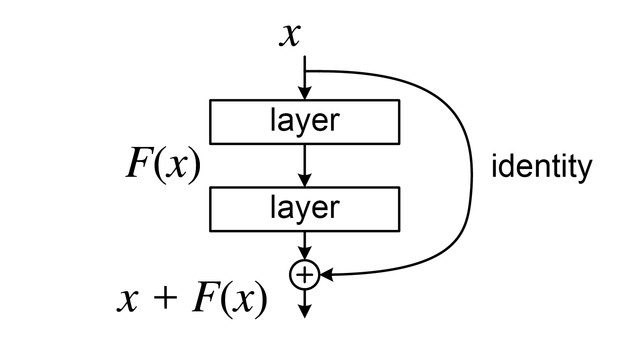
\includegraphics[width=0.55\textwidth]{Images/crossmodalnetworks/ResBlock.png}
        \caption{Image of a ResNet block.\cite{resnetpaper}}
        \label{fig:crossmodalnetworks:resblock}
    \end{figure}

    \subsection{Transformer}

    The transformer is first meantioned in \cite{attentionisallyouneed}.
    Before transformers \acrfull{rnn} were used to process sequential data.
    A mechanism called attention was used to get information about the context of a sequenz.
    The transformer was a revolution because it uses a  block called self attention.
    With this block the need for a \acrshort{rnn} is obsolet.
    \acrshort{rnn} are hard to train because of a effect called vanishing or exploding gradient.
    They are also hard to parallelize.
    These effect's no longer occure when using a transformer.


    To use a transformer the input has first to be split in tokens.
    These tokens consist of text snippets or in the case of a vision transfomer patches of a picture(see \cref{fig:crossmodalnetworks:visiontransformer}).
    These tokens then get embedded into a high dimensional vector space.
    In case of CLIP Vit32 visual encoder the vector has 1024 dimensions.
    Additionally the vectors get a postitional embedding.
    Next a combination of self attention block and feed forward is used to process the tokens (see \cref{fig:crossmodalnetworks:transformer}).
    Mutliple of these block get concantenated.

    \begin{figure}[]
        \centering
        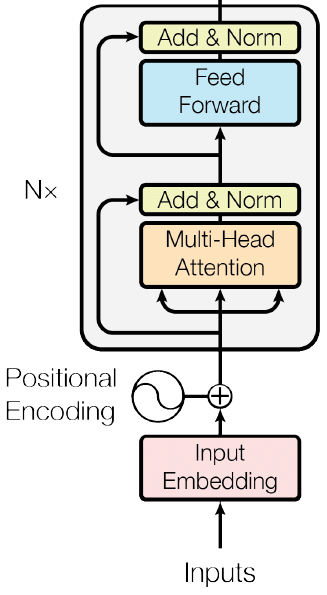
\includegraphics[width=0.25\textwidth]{Images/crossmodalnetworks/The-Transformer-encoder-structure.png}
        \caption{Image of a transformer which in the case of CLIP is used as a text encoder\cite{fig:encoder}}
        \label{fig:crossmodalnetworks:transformer}
    \end{figure}

    \begin{figure}[]
        \centering
        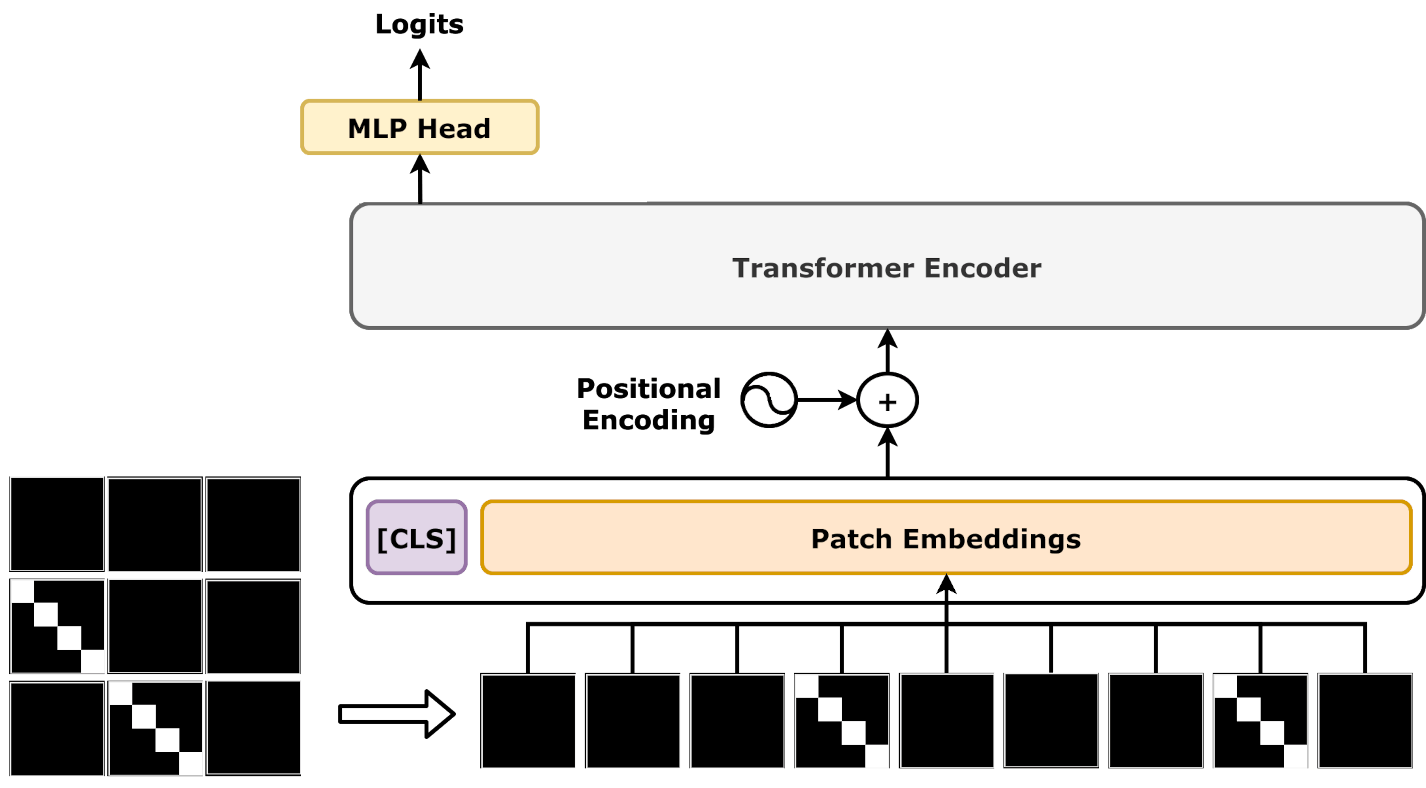
\includegraphics[width=0.6\textwidth]{Images/crossmodalnetworks/Vision_Transformer.png}
        \caption{Vision transforme architecture\cite{vitwikipedia}}
        \label{fig:crossmodalnetworks:visiontransformer}
    \end{figure}


    \section{Text encoder}
    The text encoder is in most cases a transformer.
    It encodes a given text into a high-dimensional vector space.
    This high dimensional vector space allows the encoder to correctly classify unseen classes because their vector is close to related classes.
    In theory, the closer two words are related, the closer their embedding vectors are to each other.
    An example of this can be seen in \cref{fig:crossmodalnetworks:3demb}, where \Acrfull{pca} is used to reduce the dimensions of the embedding vectors.
    Cat and dog are close together.

    \begin{figure}
        \centering
        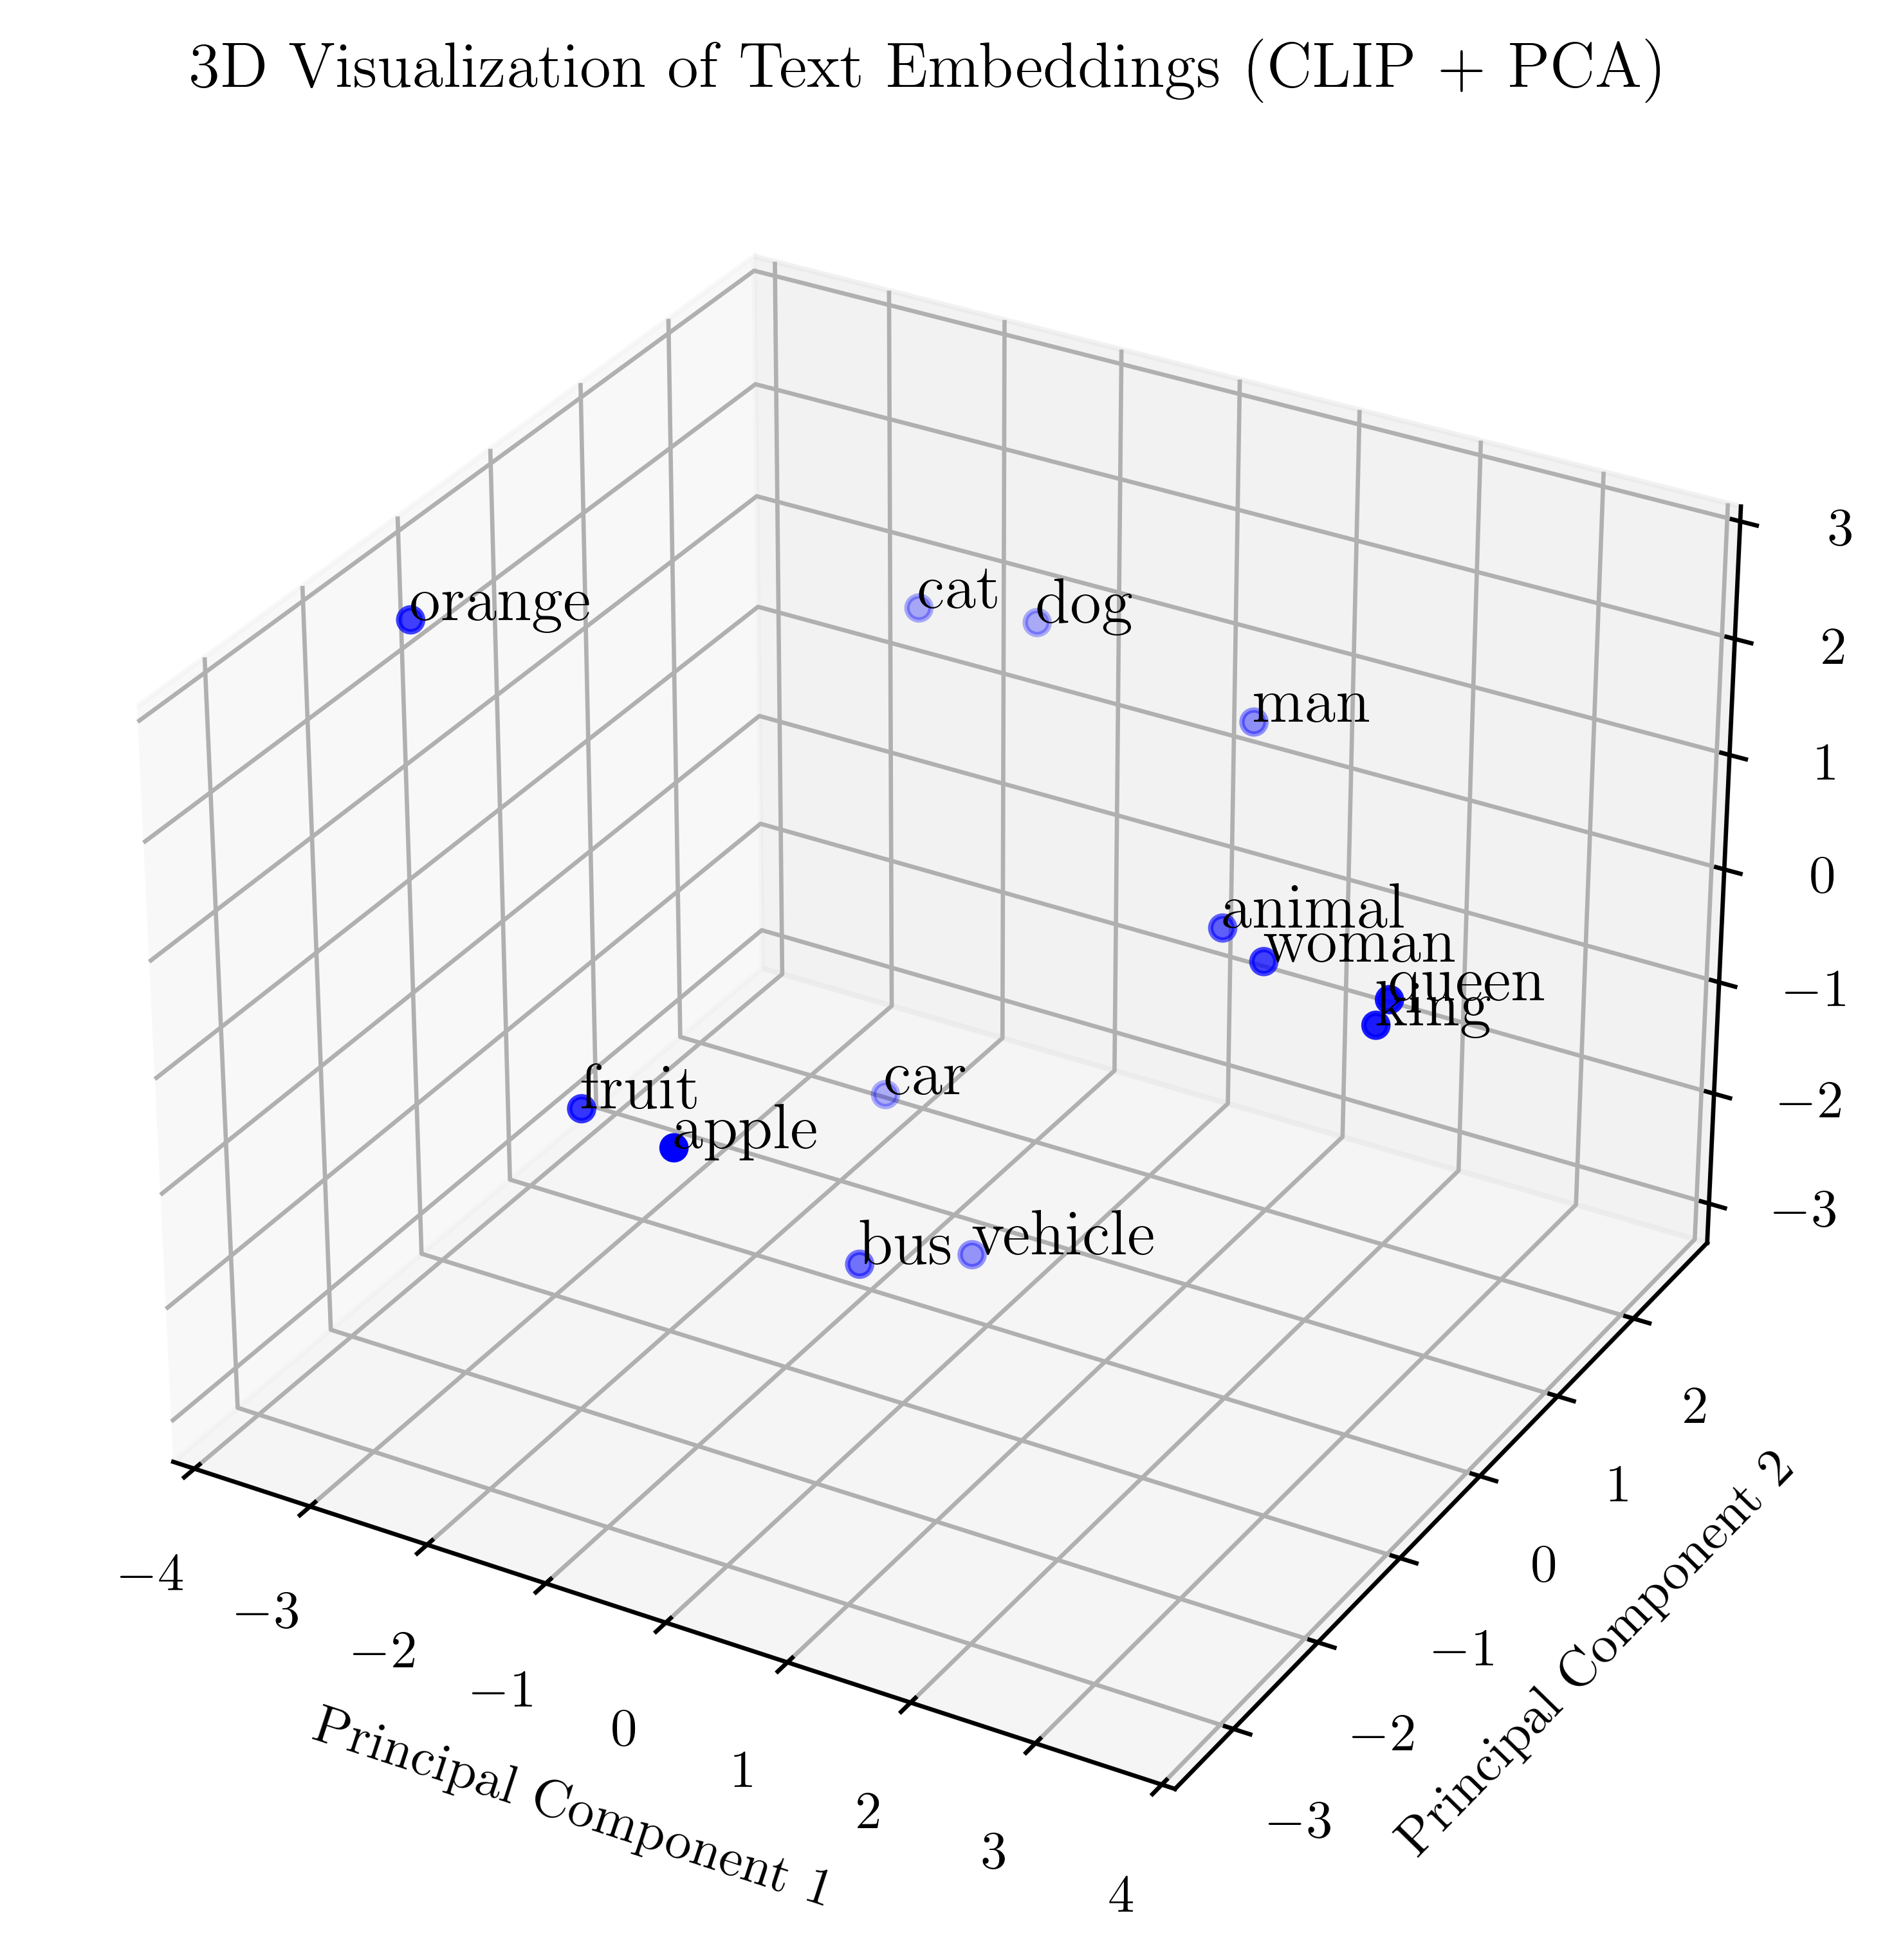
\includegraphics[width = 0.8\textwidth]{Images/crossmodalnetworks/3DEmbedding.png}
        \caption{Example of text embedding using CLIP and \Acrshort{pca}}
        \label{fig:crossmodalnetworks:3demb}
    \end{figure}
    
    \section{Image encoder}
    In most cases, the image encoder consists of a vision transformer\cite{Vis_N_Grams}.
    Like a text encoder, the vision encoder encodes an image in a high-dimensional vector space.
    A vision transformer needs an image in a specific dimension.
    For this reason, an image encoder is a pair of vision transformer and preprocessor that transforms an image into the right dimensions for the vision transformer.

    
    \section{Contrastive Language-Image models
        \label{section:languageimagemodels}}
        This section examines some models that use contrastive language-image pretraining.
        Most of the information in this section is taken from \cite{cliplikeweb} and the related papers.

        Contrastive techniques take paired inputs from two modalities (e.g. an image and its caption).
        Both inputs are embedded in their own embedding space.
        The aim is for such a pair to be represented by its corresponding encoder in a similar embedding.
        Language-image describes the two modalities used by the model.
        Most of these models are pre-trained.
        Pre-training means that the model has been trained on a large and universal dataset.
        For a specific application, a pre-trained model can be fine-tuned to better perform on its specific task.

        \subsection{CLIP
            \label{section:clip}}
        \acrfull{clip} \cite{clip} is a cross-modal model from openAI\cite{openai} that can tell how well a given image and text match.
        It can be used with a variety of image and text encoders.
        It is trained on a large dataset consisting of 400 million image-text pairs.
        It has been shown to outperform some of the best known models in classifing images.
        Many other models use CLIP as a base and build better models from it.

        \begin{figure}[]
            \centering
            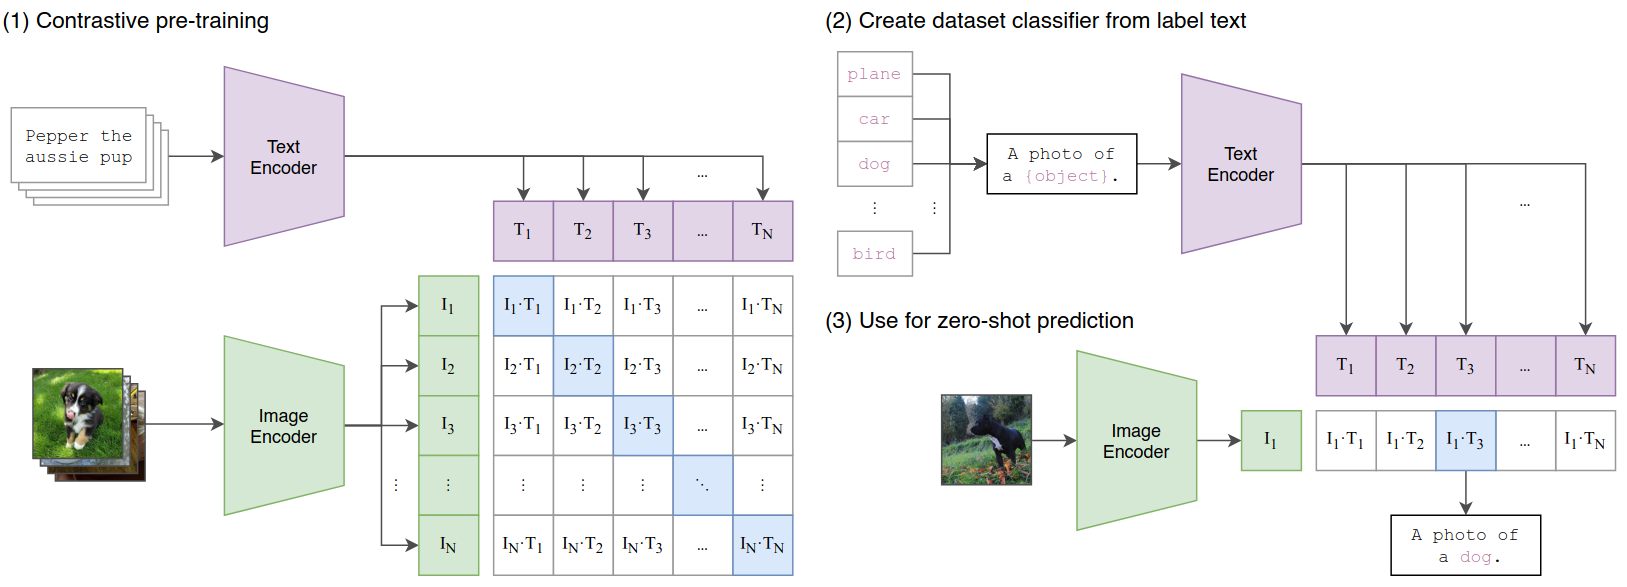
\includegraphics[width=\textwidth]{Images/crossmodalnetworks/OpenAICLIP.png}
            \caption{A picture from the \acrshort{clip} paper by OpenAI \cite{clip}.}
            \label{fig:crossmodalnetworks:openaiclip}
        \end{figure}

        \subsection{ALIGN
            \label{section:align}}
        \acrfull{align}\cite{ALIGN} was released shortly after \acrshort{clip}.
        Rather than relying on small and image caption datasets, \acrshort{align} uses a dataset of \(1.8\) billion pairs of image and alt-text pairs (e.g. in \cref{fig:crossmodalnetworks:alignepairs}).
        These alt-text descriptions are much noisier than captions.
        The authors apply basic filtering to remove duplicates, images with more than 1000 associated alt-texts, and uninformative alt-texts (either too frequent or containing rare tokens), but avoid expensive filtering operations.
        With just these simple steps, ALIGN meets or exceeds the state of the art for several zero-shot and fine-tuning tasks.
        \begin{figure}
            \centering
            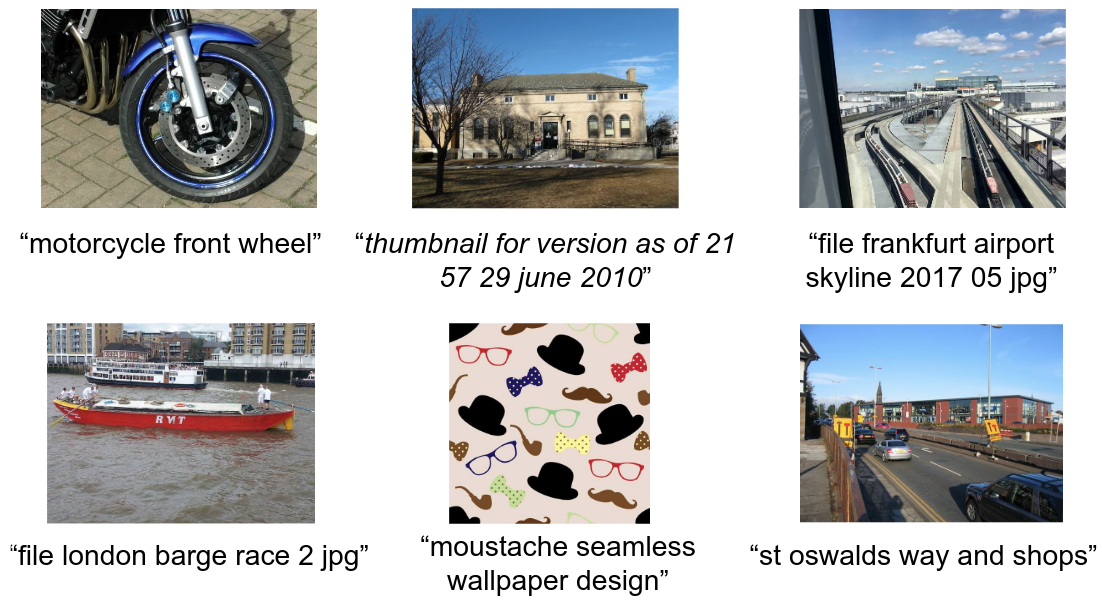
\includegraphics[width=\textwidth]{Images/crossmodalnetworks/examplepicsalign.png}
            \caption{Example of alt-text image pairs from the train dataset from \acrshort{align}\cite{ALIGN}}
            \label{fig:crossmodalnetworks:alignepairs}
        \end{figure}

        In a test for this paper, \acrshort{align} was much slower than CLIP to compute a zero-shoot evaluation on the CIFAR100\cite{cifar100} dataset.
        For 1 prediction, \acrshort{align} takes 70 times longer than \acrshort{clip} (see \cref{tab:clipaligntest}).
        Both networks are not fine-tuned. The highest predicted label is used. Due to the slow interference, ALIGN was stopped after processing 35\% of the dataset.

        \begin{table}
            \centering
            \begin{tabular}{lll}
                \hline
            \textbf{Measurment}&\textbf{ALIGN}&\textbf{CLIP}\\\hline
            Accuracy& 48.9\% & 61.7\%\\
            Speed(seconds per iterarion)&  2.16&  0.02\\ \hline
            \end{tabular}
            \caption{First test on CIFAR100.}
            \label{tab:clipaligntest}
        \end{table}

        \subsection{TinyCLIP
            \label{section:tinyclip}}
        \begin{figure}
            \centering
            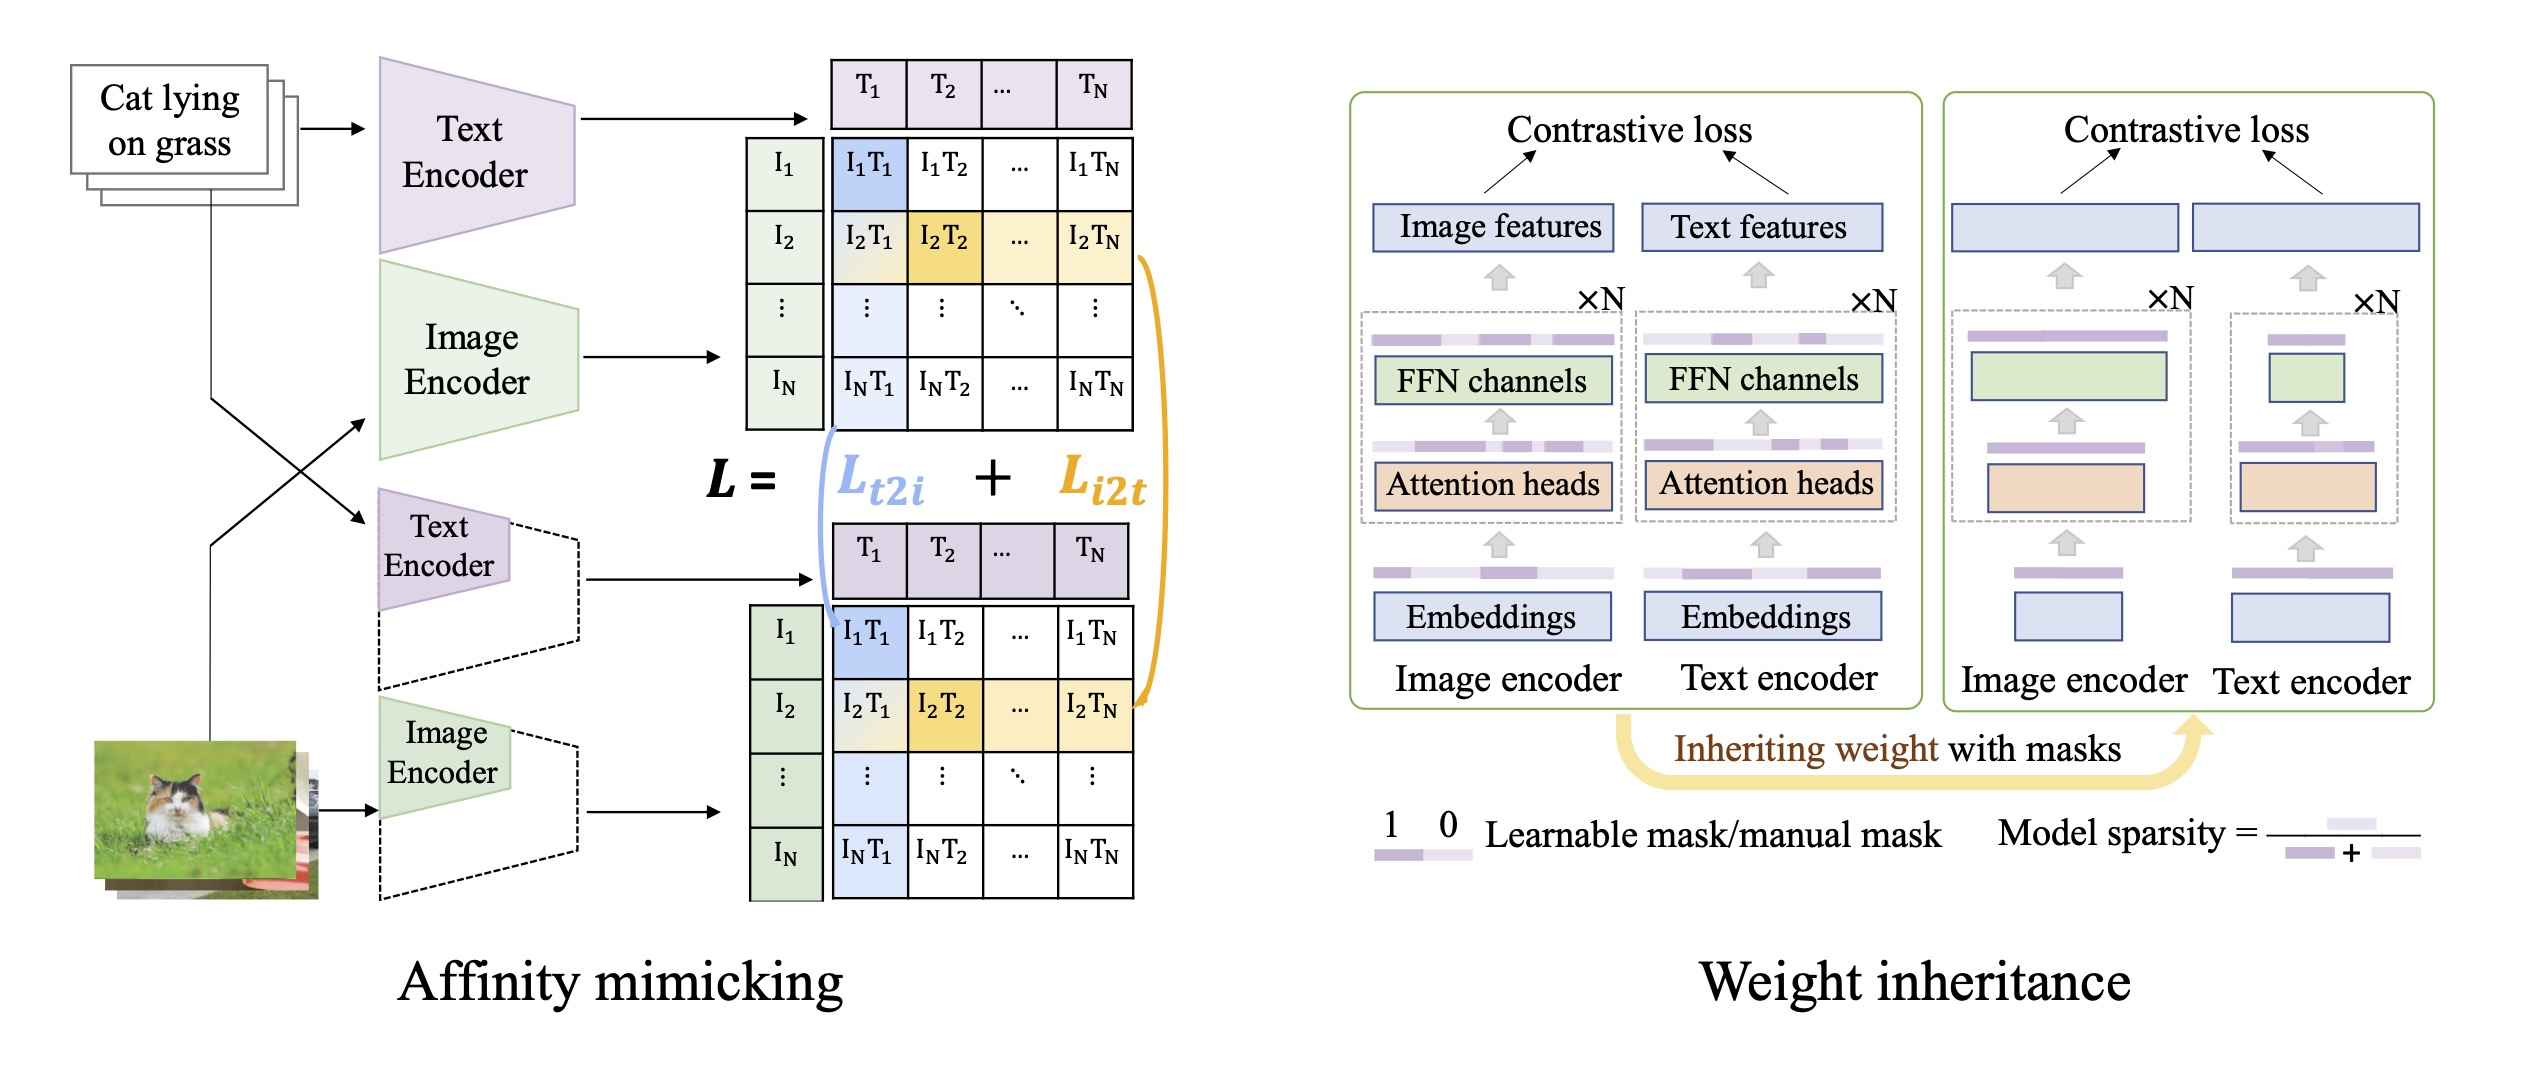
\includegraphics[width=\textwidth]{Images/crossmodalnetworks/TinyCLIP.jpg}
            \caption{Optimization which are used in TinyCLIP\cite{tinyclip}}
            \label{fig:crossmodalnetworks:tinyclip}
        \end{figure}

        TinyCLIP\cite{tinyclip} is a cross-modal distillation method for large-scale pre-trained speech-image models.
TinyClip can be used on limited systems due to its miniaturisation.
        It also speeds up training with minimal loss of model accuracy.
        It uses 3 concepts to reduce the size of the network.

        \subsubsection{Affinity mimicking}
        Affinity mimicking is a special form of knowledge distillation, also called model distillation.
        In knowledge distillation, a larger teacher network is trained first.
        After training the teacher network, a smaller student network is trained to predict the output of the teacher network.
        This works because the output of the teacher network has more information than the original label.
        Affinity Mimicking uses two new metrics in training: language-to-image loss and image-to-language loss (\(L_{t2i}\) and \(L_{i2t}\) in \cref{fig:crossmodalnetworks:tinyclip}).

        \subsubsection{Weight inhertiance}
        Weight inheritance is a technique that inherits important weights from well-trained teacher models to smaller student models.
        In the paper, the authors propose 2 methods:

        \subsubsection{Manual weight inhertiance}
        Based on the observations of the authors.
        Text encoders have most redundancy in depth (layer-wise), image encoders in width (channel-wise).
        They select \(k\) layers and channels of a branch, which will act as initialisation weights.
        To select the most important weights, some prior knowledge is required

        \subsubsection{Automatic weight inhertiance}
        The authors introduce a learnable mask to identify the importance of weight.

        \subsubsection{Multi-stage progressiv distillaiton}
        Pruning the model in several steps.
        For each stage, the authors use a modest degree of compression (e.g. 25\%). Each stage includes weight inheritance and affinity mimicking.

        % Due to the fact that TinyCLIP is already available and is much smaller in comparison to the origibal it will be further used in this work.

\section{Enhance the algorithm}

    To improve the accuracy of a pre-trained network, it can be fine-tuned to a specific task.
    Fine-tuning is a broad term.
    It ranges from the simple addition of a learnable linear layer at the end of the network to feature destillation.
    The concept of fine-tuning is derived from transfer learning\cite{transferlearning}.
    In transfer learning, the final layers of a neural network are removed and the network is retrained with new, independent layers.
    This saves time and resources.
    For example, with CLIP, a linear layer can be added to improve classification performance \cite{finetuneclip}.
    All of the fine-tuning approaches found use the output of the networks for further processing.
    Another way to increase the accuracy is to use better fitting text prompts.

    % \subsection{Probing}
    % % https://openaccess.thecvf.com/content/CVPR2024/papers/Huang_LP_A_Surprisingly_Strong_Linear_Probe_for_Few-Shot_CLIP_CVPR_2024_paper.pdf
    % \subsection{Feature destillation}
    % % https://arxiv.org/abs/2110.04544
    % \subsection{Prompt engeneering}

\section{Conclusion multi-modal networks}
    Based on the results of our own testing, ALIGN is not considered as a solution for this work.
    Instead, the focus of this work is on CLIP and TinyCLIP.
    These models can be fine-tuned to further improve their performance.
    In addition, the performance of the models can be improved by using better text prompts.
    \chapter{Market analysis
\label{chapter:marketanalysis}}

Part of this work involves conducting a market analysis of hardware accelerators with M.2 interfaces. 
The results are summarized in the attached tables, highlighting the most relevant and significant details of these products.

\section{Summary of Current Offerings}
Many hardware accelerators available today have limitations that affect their suitability.
Some products, such as the Coral M.2 accelerator, are outdated and lack the processing power.
Other products, such as the SAKURA-II M.2 and Metis M.2 cards, are still only available for pre-order, limiting their accessibility for immediate use.

From the current assessment, the Hailo products appear to be the most promising options for this project.
They offer an efficient balance of performance and power consumption, outperforming Coral's offerings in terms of TOPS (tera operations per second) while maintaining a lower power footprint.
This efficiency is critical for embedded and power-sensitive applications, making Hailo a strong candidate for further exploration and integration.

\section{Future Considerations}
Looking ahead, hardware accelerators that can handle floating-point models (FP32 or BF16) offer exciting potential.
While integer (INT8) operations are optimized for many AI applications due to their efficiency, the theoretical advantages of FP32 precision for certain tasks warrant further investigation.
However, the practical benefits of this precision shift remain to be demonstrated in many real-world use cases.


\section{Custom Design Opportunities}
An alternative to relying on off-the-shelf solutions is to design and manufacture custom PCBs with M.2 slots.
This approach enables more tailored integration and reduces dependency on proprietary vendor software.  
Many companies offer hardware accelerator chips that can be incorporated into custom designs, providing the flexibility to optimize the hardware for specific application requirements.


\section{Software Ecosystem}
In addition to the hardware, the software ecosystem that accompanies these accelerators is a critical consideration.
The entire solution, including both hardware and software, must be ready for seamless deployment.
Many companies offer end-to-end software stacks to simplify integration and accelerate development. For example:

\begin{itemize}
    \item \textbf{Hailo} offers tools such as the Dataflow Compiler \acrshort{dfc} and GStreamer/Python APIs.
    \item \textbf{Axelera} supports its products with the Voyager.SDK.
\end{itemize}

Despite these offerings, assessing the usability of software stacks during initial evaluations remains a challenge.
Most documentation and sample applications focus primarily on computer vision tasks, potentially limiting their applicability to broader use cases.
Further practical testing is required to fully understand the ease of integration and the adaptability of these tools.


\section{Detailed Tables}
The tables below summarize the economic and technical key figures of the hardware accelerators reviewed, providing a comparative overview of their capabilities and specifications.
In \cref{tab:market:keyfigures}, we see that some accelerators support BF16.
BF16 stands for Brain Floating Point with 16 bits. This format uses less space than FP32 while still being a floating-point representation.
A blank cell in the tables indicates that no information was found.

\begin{table}[!ht]
    \centering
    \begin{tabular}{|l|l|l|l|l|}
    \hline
        Product Name & Manufacturer & Price (\$) & Availability & \makecell{M.2 Slot\\Type (Key)} \\ \hline
        Hailo-8L Entry-Level M.2 Module & Hailo & 80 & Available & M, B+M, A+E \\ \hline
        Hailo-8 M.2 AI Acceleration Module & Hailo & 220 & Available & M, B+M, A+E \\ \hline
        Hailo-10H M.2 Key M & Hailo & ~ & On request & M \\ \hline
        Metis M.2 Card & Axelera & 150 & Preorder & M \\ \hline
        SAKURA-II M.2 & Edge Cortix & 249-299 & Preorder & M \\ \hline
        M.2 Accelerator & Coral & 25 & Available & B+M, A+E \\ \hline
        M.2 Accelerator Dual Edge TPU & Coral & 40 & Available & E \\ \hline
        ME1076 M.2 Accelerator Card & Mythic & ~ & On request & A+E \\ \hline
        MM1076 M.2 Accelerator Card & Mythic & ~ & On request & M \\ \hline
        MLSoC Dual M.2 Production Board & Sima.ai & ~ & On request & Dual M.2 \\ \hline
        MemryX MX3 & MemryX & ~ & On request & N.A.(Chip) \\ \hline
        Orca 1.1 M.2 & DeGirum & 159 & Available & M \\ \hline
        byteENGINE IMX8MP Plus Quad & bytesatwork & 139 & Available & N.A.(Chip) \\ \hline
        Jetson Orin Nano 4GB & Nvidia & ~ & ~ & N.A.(Chip) \\ \hline
        Jetson Orin Nano 8GB & Nvidia & ~ & ~ & N.A.(Chip) \\ \hline
        Jetson Orin Nano Developer Kit & Nvidia & ~ & ~ & N.A.(Chip) \\ \hline
        EnCharge AI Analog IMC & EnChargeAI & ~ & ~ & ~ \\ \hline
    \end{tabular}
    \caption{Economical key figures of reviewed hardware accelerators.}
    \label{tab:market:ecotable}
\end{table}

\begin{table}[!ht]
    \centering
    \begin{tabular}{|l|l|l|l|}
    \hline
        Product Name & \makecell{Processing\\Power\\(TOPS INT8)} & \makecell{Processing\\Power\\(TFLOPS FP32)} & \makecell{Power\\Consumption} \\ \hline
        Hailo-8L Entry-Level M.2 Module & 13 & ~ & 1.5 W \\ \hline
        Hailo-8 M.2 AI Acceleration Module & 26 & ~ & 2.5 W \\ \hline
        Hailo-10H M.2 Key M & 40 & ~ & 3.5 W \\ \hline
        Metis M.2 Card & 214 & ~ & 4-8 W \\ \hline
        SAKURA-II M.2 & 60 & 30 (BF16) & 10 W \\ \hline
        M.2 Accelerator & 4 & ~ & 2 W \\ \hline
        M.2 Accelerator Dual Edge TPU & 8 & ~ & 4 W \\ \hline
        ME1076 M.2 Accelerator Card & 25 & ~ & 3.5 W \\ \hline
        MM1076 M.2 Accelerator Card & 25 & ~ & 3.5 W \\ \hline
        MLSoC Dual M.2 Production Board & 50 & ~ & 15 W \\ \hline
        MemryX MX3 & ~ & 5 (BF16) & ~ \\ \hline
        Orca 1.1 M.2 & ~ & ~ & 4.5 W \\ \hline
        byteENGINE IMX8MP Plus Quad & 2.3 & ~ & 33 W \\ \hline
        Jetson Orin Nano 4GB & 20 & ~ & 7-10 W \\ \hline
        Jetson Orin Nano 8GB & 40 & ~ & 7-15 W \\ \hline
        Jetson Orin Nano Developer Kit & 40 & ~ & 7-15 W \\ \hline
        EnCharge AI Analog IMC & 150  & ~ & ~ \\ \hline
    \end{tabular}
    \caption{Key technical figures of reviewed hardware accelerators.}
    \label{tab:market:keyfigures}
\end{table}

    \chapter{Hardware Accelerator}

The Raspberry Pi 5 with an Ai kit was chosen as the hardware to prove the concept of computing data at the edge.
This desiction was taken based on recommendations from the advisors and the avilability.
The market analysis confirms this choice.
The hardware accelerator of the Ai kit is made by Hailo \cite{hailo}.
Generally a hardware accelerator is used to compute neural netwroks like a graphics card is used to compute graphics.
Hailo is a company which produces hardware accelerators.
The Ai kit uses the Hailo-8L entry level hardware accelerator.
Hailo provides a pipeline to compile a network so that it can be executed on the hailo software.
First we take a look at the compilation of a network which has to be done on a PC, 
preferibly one with a GPU.
Secondly were looking on the way to run the network on the edge.

\section{Network compilation}
As sad before, the network has to be precompiled on a PC.
The application which is meant for this task is called the \Acrfull{dfc}.

\subsection{Dataflow compiler
\label{section:dfc}}

To use the \acrshort{dfc} a pytorch or tensorflow model has to be converted to Onnx or tensorflow light.
Information and pictures are taken from the Hailo Dataflow Compiler User Guide\cite{hailo_dataflow_compiler}.
The \acrshort{dfc} the compiles the model to a \Acrfull{hef} by executing the following steps:

\begin{enumerate}
    \item Full Precision Optimization
    \item Quantization Optimization
    \item Compilation
\end{enumerate}
In the full precision optimization step ONNX file first gets compiled into a \acrfull{har} file, a file type defined by Hailo.
This step also includes any changes to the model in the floating-point precision domain, for example Equalization\cite{meller2019same}, \acrshort{tse}\cite{Vosco_2021_ICCV} and pruning.

In the quantization optimization step the model gets compressed.
This means that the model gets converted from floating point to integer.
Weights get compiled to either 4,8 or 16 bits.
Activaitions get compiled to 8 or 16 bits.
Which quantisation is applied is handeled through a model script.
In that script the amount of quantized weights can be described.
There is also the posibility to target specific layer by the model script.
It is also possible to add preprocessing steps to the model script like resize the input or convert the input from RGB to YUV.
The result of this step is a quantized \acrshort{har} file.
This file can be compiled to a \acrshort{hef} file to use the model on Hailo hardware.

\begin{figure}[!h]
    \centering
    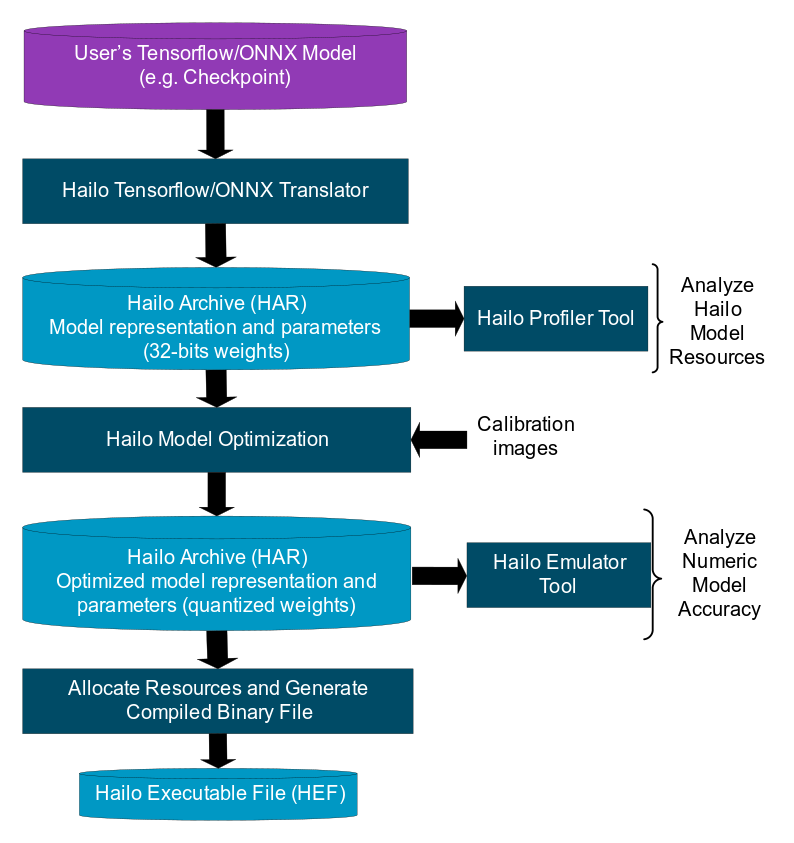
\includegraphics[width=\textwidth]{Images/Hardware/model_build_overview_with_onnx_and_hef_w_har.png}
    \caption{\Acrlong{dfc} overview \cite{hailo_dataflow_compiler}}
    \label{fig:hardware:dfcoverview}
\end{figure}

\subsection{Constrains}
At the time of this writing, the \acrshort{dfc} is not capable of compiling Transformers.
This is a very important limiting factor for this porject.
The best performance for CLIP is achieved with vision Transformers as image encoder.
Fortunately, the visual encoding of CLIP can also be done with ResNet, a special form of \Acrshort{cnn}'s.

\section{Running on the edge}

Hailo provides a library called TAPPAS which is based on GStreamer.
The library enables using a Hailo device within gstreamer pipelines t create intelligent video processing applications.
The information for this section are taken from the TAPPAS User Guide.
In the point of time there are two approaches to run a network on a hailo device.
One with Gstreamer and one with a Python API.
There are many different example applications available for many diffrent usecases.
These examples can be found in the Hailo model zoo\cite{hailo_model_zoo} or in their repo for Raspberry Pi examples \cite{hailo_rpi5_examples}.


\subsection{GStreamer approach}

Gstreamer is a framework for creating streaming media applications.
It enables the design any type of multimedia application but it isnt restridted to audio and video processing.
The framework can porcess any kind of dataflow.

GStreamer consists of blocks which can be concantenated.
To work with the Hailo hardware accelerator some blocks in the pipeline get offloaded to the Hailo processor.
A python programm is used to construct a string which then is executed in a terminal.
A example pipeline can be seen in \cref{fig:hardware:gstreamerpipeline}.
More examples with code can be found in the TAPPAS User Guide.
\begin{figure}[!h]
    \centering
    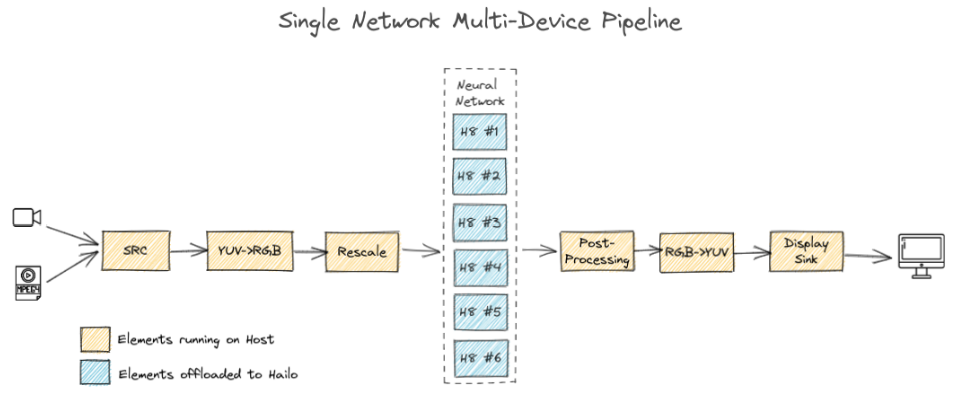
\includegraphics[width=\textwidth]{Images/Hardware/gstreamerExample.png}
    \caption{Example GStreamer pipeline from TAPPAS User Guide}
    \label{fig:hardware:gstreamerpipeline}
\end{figure}

\subsection{Python API approach}

With the Python API approch one can execute the whole inferance in python.
That makes the programm very simple in comparison to the GStreamer approach.
In python the Hailo hardware accelerator gets treated as an object with dedicated functions to use inference.
Importent to know is that hailo swaps the input dimension of the network.
This menas that the dimensions of the input to the network has to be adjusted.
Due to complexity of the GStreamer approch the Python API is used in this project.
    \chapter{System Overview}

The goal of the system is to classify panorama images into predefined classes.  
For this, a CLIP-like network is used at the edge.  
The computing platform consists of a Raspberry Pi 5 with the hardware accelerator extension.  
The hardware accelerator is the Hailo-8L entry-level accelerator (\cref{fig:overview:aikit}).  

The system used and developed in this work can be divided into two parts.  
One part involves compiling a neural network on a PC,  
while the other part focuses on running the inference of the compiled network on the Raspberry Pi.

\begin{figure}[h]
    \centering
    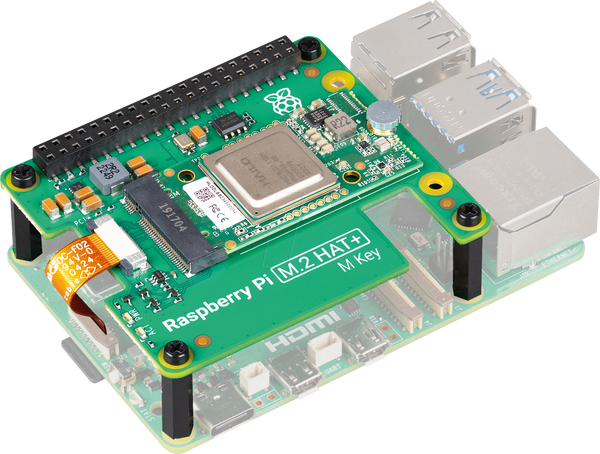
\includegraphics[width=0.5\textwidth]{Images/SystemOverview/ai-kit.png}
    \caption{Picture of the hardware accelerator mounted on a Raspberry Pi 5\cite{bildAiKit}}
    \label{fig:overview:aikit}
\end{figure}



\section{Compilation of a Network}

\begin{figure}
    \centering
    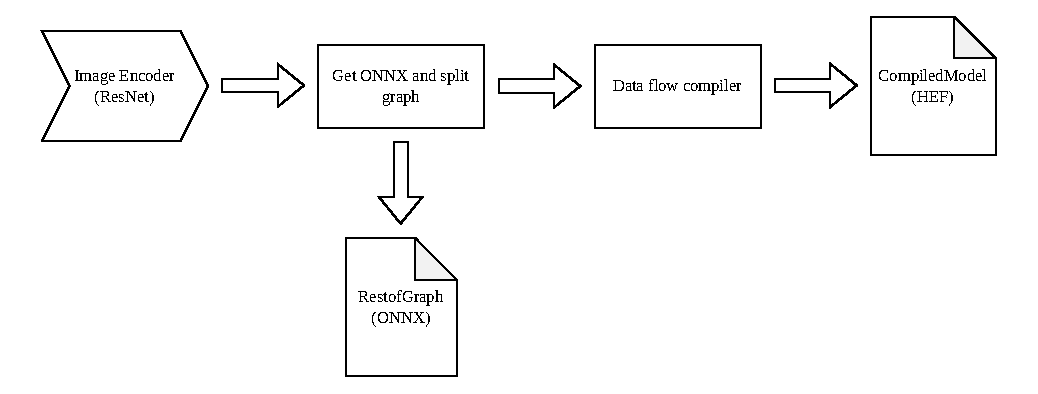
\includegraphics[width=\textwidth]{Images/SystemOverview/DFCFlow.pdf}
    \caption{Visualization of the compilation workflow}
    \label{fig:overview:dfcflow}
\end{figure}

First, the image encoder, either from \acrshort{clip} or TinyCLIP, must be acquired.  
This encoder is then exported as an ONNX graph.  
Any part of the graph that cannot be compiled is removed and saved for later use.  
The edited graph is then compiled.  
During compilation, the network undergoes quantization and simplification.  
This reduces the memory and processing power required to run the network.  

The network must be compiled into a format that can be executed on the hardware accelerator.  
In this work, the compilation is performed using the \Acrlong{dfc} (see \cref{section:dfc}) from Hailo.  
The result is a \acrshort{hef} file, which can be executed on Hailo hardware.


\section{Inference on Raspberry Pi}

\begin{figure}
    \centering
    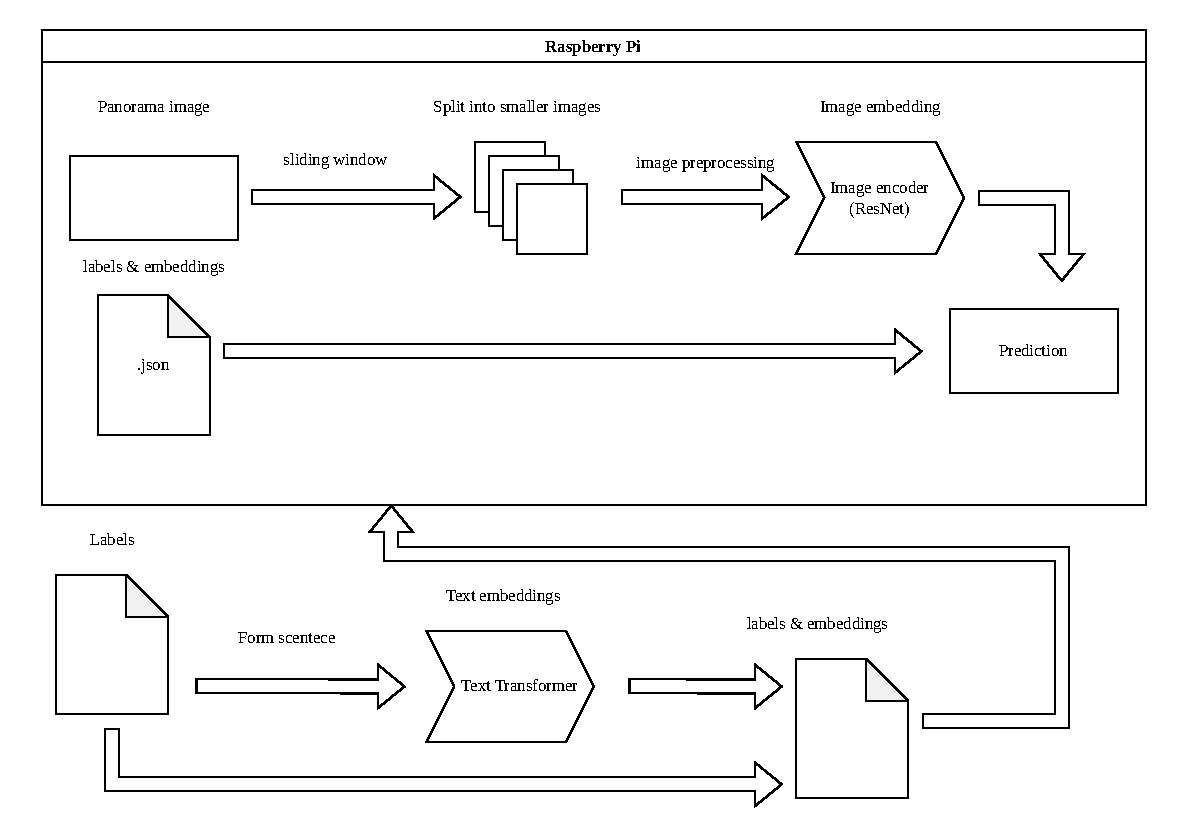
\includegraphics[width=\textwidth]{Images/SystemOverview/Overview.drawio.pdf}
    \caption{System workflow}
    \label{fig:overview:overview}
\end{figure}

To use a network on a hardware accelerator, specific software must be employed.  
Due to current limitations of the \acrshort{dfc}, self-attention layers were unable to compile.  
As a result, the text encoder of CLIP must be executed in advance on a PC.  
The resulting text embeddings are then loaded onto the Raspberry Pi in the form of a JSON file.  
The text embeddings consist of the expressions from \cref{tab:dataset:subclasses} subclasses.  
These expressions are wrapped into 5 sentences to improve accuracy.  

This limitation also prevents the compilation of transformers.  
Therefore, ResNets were used as the image encoders.  
However, a challenge arose with ResNets, as the last layer is also a self-attention layer.  
To enable the network to compile, the last part of the ResNet was removed and processed later as part of postprocessing.  

The panorama images are divided into 5 separate patches, each classified individually.  
To obtain the final prediction, a majority vote is taken across the 5 image patches.



    \chapter{Hexagon Dataset
    \label{chapter:dataset}}
Most of the information for this chapter is taken from Lia Winklers master thesies.
The dataset was collected using the terrestrial laser scanner RTC 360 from Leica at 32 different locations.
In total, this dataset consists of 821 clean images and the number of images per location ranges from 4 to 423.
All the images are 360-degree panoramas with a
resolution of 8192 \(\times\) 4096 pixels.
The images are divided into the following 5 classes:

\begin{itemize}
    \item Indoor architectural
    \item Indoor construction
    \item Outdoor construction
    \item Outdoor Urban
    \item Forest
\end{itemize}

\noindent
To increase the accuracy of the algorithem the classes got rephrased and divided in subclasses.
These subclasses can be seen in \cref{tab:dataset:subclasses}.
\begin{table}[!ht]
    \centering
    \begin{tabular}{ccc}
    \toprule
    \textbf{1. Original}& \textbf{2. Rephrased}& \textbf{3. Subclasses}\\ \midrule
    Construction (in) & construction site & \makecell{construction site,\\ mining, tunnel}\\ \hline
    Architectural (in)& architectural& \makecell{architectural, office,\\ residential, school,\\ manufacturing, cellar,\\ laboratory} \\ \hline
    Construction (out)& construction site & construction site \\ \hline
    Urban (out)& town & \makecell{town, city,\\countryside, alley,\\ parking lot} \\ \hline
    Forest (out)& forest& forest \\
    \bottomrule
    \end{tabular}
    \caption{Rephrased terms and their subclasses
        \label{tab:dataset:subclasses}}
\end{table}

\begin{table}
    \centering
    \begin{tabular}{cc}
    \toprule
    \textbf{Class}& \textbf{Picture Classes}\\ \midrule
    Construction (in) & 9,13,39,12 \\ \hline
    Architectural (in)& 7,10,18,27,29,32,36,1,28,6,33,40,30,31,24\\ \hline
    Construction (out)& 8,16,22\\ \hline
    Urban (out)& 2,20,38,26,15,42,44,4,23\\ \hline
    Forest (out)& 17\\
    \bottomrule
    \end{tabular}
    \caption{Picture Classes of the hexagon dataset
        \label{tab:dataset:piccoding}}
\end{table}

The labels of the pictures are in the name of the picture.
The first number is the location where the picture was taken.
The second number is a sequential number for that location.
The \cref{tab:dataset:piccoding} tell you which class corresponds to which location.
For example the picture from \cref{fig:dataset:examplepic} is from the class Construction (in).

It is important to mention that the dataset is highly imbalanced.
Nearly 80\% of the panorama images are from the class indoor architectural.
This means that a "stupid" model can achieve a accuracy of 80\% by labeling every input as indoor architectural.
It is important to incoparate this fact in the evaluation of the performance of a model.

\begin{figure}
    \centering
    \includegraphics[width=\textwidth]{Images/Dataset/panorama_00009_0015.jpg}
    \caption{Example picture from the hexagon dataset [panorama\_00009\_0015.jpg]}
    \label{fig:dataset:examplepic}
\end{figure}


    \chapter{Implementation
    \label{chapter:implementation}}

This chapter discribs the tools, methods and reasons for the from of implementation.
As sad due to early test CLIP and TinyCLIP are used as models.

\section{Model acquisition}

The CLIP models are taken from the official CLIP Github repo \cite{clipgit}.
The TinyCLIP models are taken from the official TinyCLIP Github repo \cite{tinyclipgit}.
There is also the posibility to take models from HuggingFace \cite{huggingface}.
The problem with HuggingFace is that the model cant be split into image and text encoder.
Because of this reason only models from the offical CLIP respectiv TinyCLIP repo were used.
In \cref{tab:methods:clipsize} one can see the parameter count for all CLIP and TinyCLIP implementation which use a ResNet as a visual encoder.
We see that TinyCLIP 
\begin{table}[h]
    \centering
    \begin{tabular}{lll}
    \hline
    Model name & \begin{tabular}[c]{@{}l@{}}Parameters\\ Visual(Mio)\end{tabular} & \begin{tabular}[c]{@{}l@{}}Parameters\\ Text(Mio)\end{tabular} \\ \hline
    RN50                & 38  & 38  \\
    RN50x4              & 87  & 59  \\
    RN50x16             & 167 & 850 \\
    RN50x64             & 420 & 151 \\
    RN101               & 56  & 38  \\
    TinyCLIP-ResNet-19M & 19  & 19  \\
    TinyCLIP-ResNet-30M & 30  & 29  \\ \hline
    \end{tabular}
    \caption{Paramter count for different CLIP implementations with ResNet as visual encoder}
    \label{tab:methods:clipsize}
\end{table}

\section{Model translation}
The models were first split into image and text encoder.
The image encoder then gets translated to a onnx graph and afterwards simplified.
This onnx graph then is translated by the \acrshort{dfc} to \acrshort{har} and \acrshort{hef} files.

\begin{figure}
    \centering
    \subfloat[End of CLIP ResNet50x4 vision encoder Onnx graph acquired though official CLIP]{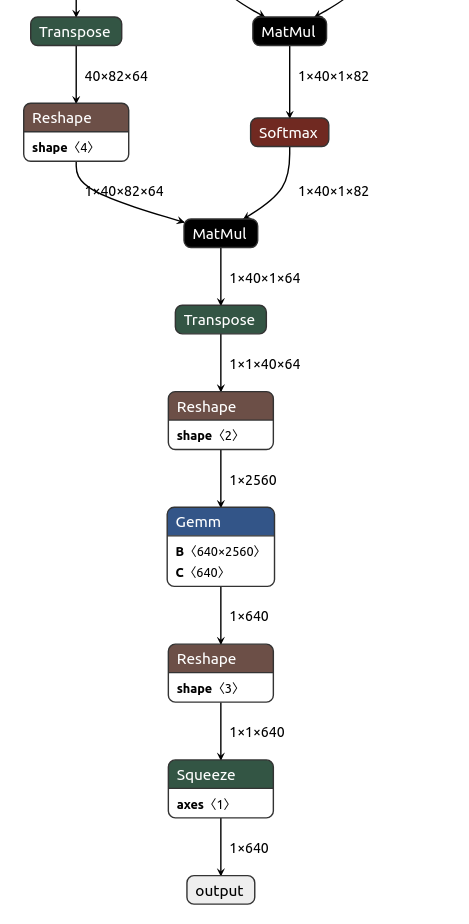
\includegraphics[width=0.4\textwidth]{Images/Implementation/ClipRes50x4.png}\label{fig:implementation:clipres50x4}}
    \qquad
    \subfloat[End of CLIP ResNet 50x4 vision encoder Onnx graph sendt by Hailo]{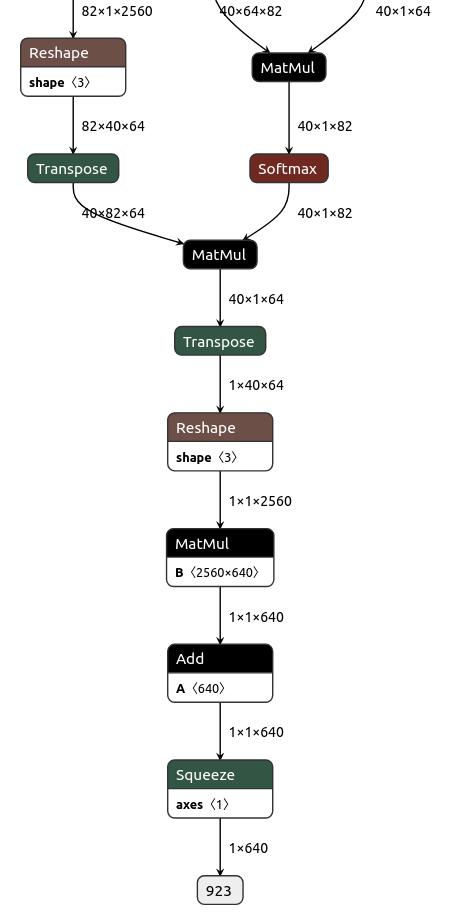
\includegraphics[width=0.4\textwidth]{Images/Implementation/HailoClipRes50x4.png}\label{fig:implementation:hailoclipres50x4}}
    \caption{Comparison of CLIP ResNet 50x4 vision encoder Onnx graph (a) from official CLIP and (b) from Hailo}
    \label{fig:implementation:compareRN50x4}
\end{figure}

In that step lays the first big problem of the project.
As described in \cref{section:dfc} the \acrshort{dfc} is unable to compile transformers.
To be precise, a transpose block at the end of every self attention layer is were the problems lay.
The \acrshort{dfc} swaps dimensions and takes together the last 2 dimensions.
In the ResNet which is acquired though the offical code (see \cref{fig:implementation:clipres50x4}) one can see that the transpose block after the MatMul block swaps a second and the third dimension.
This leads to a compilation error because the \acrshort{dfc} already combined the last 2 dimensions.
This error does not occure when the model given by Hailo is compiled.
In \cref{fig:implementation:hailoclipres50x4} the maximum of dimensions is 3.

To work around this problem the last part of the onnx graph is cut off.
To cut the graph Onnx-Modifier \cite{onnxmodifier} is used.
The cut off blocks are implemented as postprocessing.
As described in \cref{section:dfc} a script can be applied to change the behavior of the \acrshort{dfc}.
% Add scripts

After quantisation the graph can again be visualized with a tool name profiler from hailo.
In \cref{fig:implementation:compareRN50x4qunathar} the compiled model with the cutoff end is visualized.
In this figure the combination of the last dimensions can be seen.

\begin{figure}
    \centering
    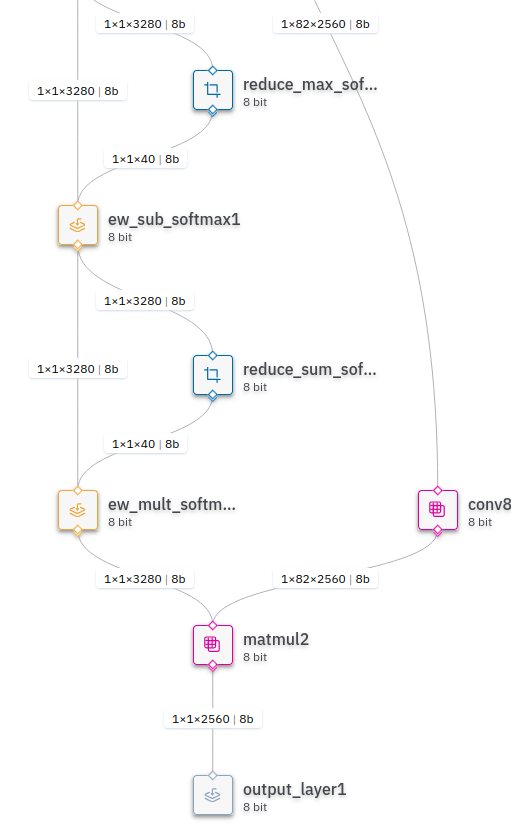
\includegraphics[width=0.4\textwidth]{Images/Implementation/ClipRes50x4_qunat_Har.png}
    \caption{Output of the \acrshort{dfc} from compiling the modified onnx graph of the ResNet50x4.}
    \label{fig:implementation:compareRN50x4qunathar}
\end{figure}

This graph then gets compiled to a \acrshort{hef} file which can be executed on Hailo hardware.
To use CLIP the text embeddings are also needed.
Due to the limitation that no transformers can be used with hailo the embeddings get calculated on a PC and the saved in a Json file.

\textbf{Comparison size}


\subsection{Pre-processing}

The hexagon dataset which is used as refrence consists of panorama pictures.
These pictuers get cut into 5 equal sized patches.
Every patch gets processed with CLIP.
To finally classify a image a mayority vote is taken over the subclasses of the patches.
This process is mentiond in Lia Winkler's report and increases the accuracy of the model.

\subsection{Post-processing}

As sad the cut of part of the Onnx graph is processed in post processing.
The Cut of part consists of one matrix multipication and some rearanging of the dimensions.
In a first implementation the weights for the matrix multipication were extracted and saved in a json file.
In a second attemp the cut off Onnx Graph is directly used.
The second attemp proved as faster while using much less memory.

\section{Inference}
To have a good comparison of performance the implementation on the Raspberry Pi is mostly similar to the one which is used on PC.
The PC application is mostly the same as Lia Winkler used in her work.
For Vision encoder only ResNet's were used because of the limitations from the \acrshort{dfc}.
The Hexagon dataset is used as image input.
As text input the subclasses from \cref{tab:dataset:subclasses} are used.
The text input were used solo or in a scentens.
In \cite{clip} the authors state that the performance of the network can improve if the text inputs are in a scentens.
To use the vision model on Hailo the python api is used.
2 diffrent implmentations were tested.
One proved much slower because the device initialisation happens every time a image is encoded.


To check the functionalit of the \acrshort{dfc} as test picture is used.
The \acrshort{dfc} is able to calculate the output of the compiling network at every step.
This is used to compare the output of the different stages with a test image.
The Results can be seen in \cref{tab:methods:clipcompare}.

\begin{table}[]
    \centering
    \begin{tabular}{llllll}
    \hline
    Labels        & a Human & a Cat   & a Dog  & a white cat & a small dog \\ \hline
    Original      & 1.57 \%  & 90.65 \% & 0.34 \% & 7.23 \%      & 0.2 \%       \\
    Nativ \acrshort{har}        & 1.57 \%  & 90.65 \% & 0.34 \% & 7.23 \%      & 0.2 \%       \\
    Compiled \acrshort{har}     & 1.57 \%  & 90.65 \% & 0.34 \% & 7.23 \%      & 0.2 \%       \\
    Qunatized \acrshort{har}    & 1.9 \%   & 90.10 \% & 3.49 \% & 3.63 \%      & 0.8 \%       \\ \hline
    \end{tabular}
    \caption{Output probabilitys of test image at diffrent \acrshort{dfc} stages with CLIP RN50x4 as image encoder}
    \label{tab:methods:clipcompare}
\end{table}

\begin{table}
    \centering
    \begin{tabular}{llllll}
    \hline
    Labels        & a Human & a Cat & a Dog & a white cat & a small dog \\ \hline
    Original      &         &       &       &             &             \\
    Nativ \acrshort{har}     &         &       &       &             &             \\
    Compiled HAR  &         &       &       &             &             \\
    Qunatized HAR &         &       &       &             &                   
    \end{tabular}
    \caption{Output probabilitys of test image at diffrent \acrshort{dfc} stages
    \label{tab:methods:tinyclipcompare}}
\end{table}

As suspected the accuracy reduces significant after quantisation.


\section{Measurments}

To measure the performance of the Hailo hardware the models were tested in 3 ways:
\begin{itemize}
    \item CPU PC
    \item CPU Raspberry Pi
    \item Hailo hardware accelerator
\end{itemize}

As values to measure the following found usefull:
\begin{itemize}
    \item Throughput(speed)
    \item Mermory(size)
    \item Accuracy
\end{itemize}
The implementations were made as similiar as possible to ensuer the values are correct. 

% classes = ["construction site", "town", "city",
% "country side", "alley", "parking lot", "forest"]

% === CLIP PC ===
% Label probs: tensor([[0.1811, 0.0591, 0.0398, 0.0643, 0.5045, 0.0731, 0.0782]])

% === CLIP ONNX ===
% Label probs: tensor([[0.1811, 0.0591, 0.0398, 0.0643, 0.5045, 0.0731, 0.0782]])

% === CLIP HAR Nativ ===
% Label probs: [[0.18112072348594666, 0.05905136093497276, 0.03980713337659836, 0.06425424665212631, 0.5045444965362549, 0.07307031750679016, 0.07815175503492355]]

% === CLIP HAR Compiled ===
% Label probs: [[0.1811216175556183, 0.05905177444219589, 0.03980710357427597, 0.06425445526838303, 0.5045422315597534, 0.07307054847478867, 0.07815229147672653]]

% === CLIP HAR Quantized ===
% Label probs: [[0.11425743252038956, 0.05362681299448013, 0.04226280003786087, 0.07041049748659134, 0.47000423073768616, 0.1376064419746399, 0.11183185130357742]]


% === TinyCLIP PC ===
% Label probs: tensor([[4.0224e-05, 9.6976e-02, 8.2027e-01, 1.2005e-06, 8.2412e-02, 2.9768e-04,
%          1.0994e-06]])

% === TinyCLIP ONNX Modified ===
% Label probs: tensor([[4.0224e-05, 9.6976e-02, 8.2027e-01, 1.2005e-06, 8.2412e-02, 2.9768e-04,
%          1.0994e-06]])

% === TinyCLIP ONNX ===
% Label probs: tensor([[[4.0224e-05, 9.6976e-02, 8.2027e-01, 1.2005e-06, 8.2412e-02,
%           2.9768e-04, 1.0994e-06]]])

% === TinyCLIP HAR Nativ ===
% Label probs: [4.022434586659074e-05, 0.0969763770699501, 0.8202731609344482, 1.2005439202766865e-06, 0.08241038769483566, 0.00029767947853542864, 1.0993793466695934e-06]

% === TinyCLIP HAR Compiled ===
% Label probs: [4.022362918476574e-05, 0.09697584807872772, 0.8202733993530273, 1.2005442613371997e-06, 0.08241056650876999, 0.00029767389059998095, 1.099363998946501e-06]

% === TinyCLIP HAR Quantized ===
% Label probs: [3.652078885352239e-05, 0.021380390971899033, 0.9444331526756287, 0.006429065950214863, 0.02356742136180401, 0.0007093786844052374, 0.003444116795435548]
    \chapter{Results}
In this chapter the results and their collection is discussed and interpreted.

\section{Evaluation}

To measure the performance of the Hailo hardware the models were tested in 3 ways:
\begin{itemize}
    \item CPU PC
    \item CPU Raspberry Pi
    \item Hailo hardware accelerator
\end{itemize}
The implementations were made as similiar as possible to ensuer the values are correct and representiv. 
As values to measure the following found usefull:
\begin{itemize}
    \item Throughput(speed)
    \item Accuracy
    \item Mermory(parameter count and size) 
\end{itemize}

For throughput 2 measurments are taken.
The first measures the time from input to output.
This includes calculating the text embeddings, the image embeddings and the dot product of the embeddings.
This measurment is called throughput and is measured in iterations per second (it/s).
The second measures the time it takes to calculate one image embedding.
This measurment is called throughput image and is also measured in iterations per second (it/s).

The accuracy of a model describes how a model performs in labeling pictures as in- or outdoor.
This measurment is taken because it is an easy way to see if a network is working correct but it can easly give a wrong image of the situation because it doesnt take unbalanced datasets in conciredation.
To get a precise answer if the network is working correct the confusion matix or a class report of a model has to evaluated.
Both of these are found in the appendix.

The models get executed on the edge.
Although a Raspberry Pi has plenty of mermory it is always a good practice to include the size of a model as measurment.
Size is measured in memory or parameter count.

\subsection{Without hardware accelerator}
In \cref{result:tab:perfPC} the performance on a PC CPU is displayed.
These values 
These values are used to compare the performance with the hailo hardware accelerator.

\begin{table}[]
    \centering
    \begin{tabular}{l|rrrrr}
    \hline
        Modelname & Accuracy & \makecell{Throughput\\(it/s)} & \makecell{Throughput \\ Image (it/s)} & Throughput std & \makecell{Throughput\\Image std} \\ \hline
        RN50 & 0.982 & 12.46 & 32.48 & 5.33 & 3.18 \\ 
        RN101 & 0.984 & 9.38 & 20.01 & 3.43 & 1.81 \\ 
        RN50x4 & 0.989 & 5.79 & 12.13 & 2.04 & 0.86 \\ 
        RN50x16 & 0.963 & 2.51 & 3.81 & 0.55 & 0.17 \\ 
        RN50x64 & 0.988 & 0.88 & 1.13 & 0.11 & 0.03 \\ 
        TinyCLIP-19M & 0.985 & 20.38 & 54.06 & 8.37 & 3.65 \\ 
        TinyCLIP-30M & 0.988 & 13.59 & 37.53 & 5.72 & 3.31 \\ 
    \end{tabular}
    \caption{Performance table from evalutaion on PC CPU.}
    \label{result:tab:perfPC}
\end{table}

In \cref{result:tab:perfRaspi} the performance measurments from executing on the Raspberry Pi CPU are displayed.
RN50x16 and RN50x64 are missing because they are too big to evaluate.
As one can expect the throughput on the Raspberry Pi is significant lower than the throughput on the PC CPU from \cref{result:tab:perfPC} because of the lower computing power.
Intresting is that the accurcy from \cref{result:tab:perfRaspi} is slightly different to \cref{result:tab:perfPC}.
This can be explaind by diffrent CPU architectures and some floating point rounding.
In {result:tab:perfRaspi} the parameter count of the image encoder is displayed. These values are the same for the models on PC and Raspberry Pi.
\begin{table}[]
    \centering
    \begin{tabular}{l|rrrrr}
    \hline
    Modelname & Accuracy & \makecell{Throughput\\(it/s)} & \makecell{Throughput \\ Image (it/s)} & Throughput std & \makecell{Throughput\\Image std} \\ \hline
        RN50 & 0.979 & 1.15 & 2.85 & 0.36 & 0.05 \\ 
        RN101 & 0.982 & 0.92 & 1.89 & 0.24 & 0.038 \\ 
        RN50x4 & 0.988 & 0.61 & 1.13 & 0.14 & 0.0162 \\ 
        TinyCLIP-19M & 0.982 & 2.27 & 5.22 & 0.63 & 0.16 \\ 
        TinyCLIP-30M & 0.983 & 1.60 & 3.79 & 0.47 & 0.09 \\ 
    \end{tabular}
    \caption{Performance table from evalutaion on Raspberry Pi CPU.}
    \label{result:tab:perfRaspi}
\end{table}

\begin{table}[h]
    \centering
    \begin{tabular}{l|rr}
    \hline
    Model name & \begin{tabular}[c]{@{}l@{}}Parameters\\ Visual(Mio)\end{tabular} & \begin{tabular}[c]{@{}l@{}}Parameters\\ Text(Mio)\end{tabular} \\ \hline
    RN50                & 38.3  & 37.8  \\
    RN50x4              & 87.1  & 59.1  \\
    RN50x16             & 167.3 & 850.5 \\
    RN50x64             & 420.4 & 151.1 \\
    RN101               & 56.3  & 37.8  \\
    TinyCLIP-19M & 18.5  & 18.9  \\
    TinyCLIP-30M & 29.5  & 28.3  \\ 
    \end{tabular}
    \caption{Paramter count for different CLIP implementations with ResNet as visual encoder}
    \label{result:tab:clipsize}
\end{table}



\subsection{With hardware accelerator}
\begin{table}[h]
    \centering
    \begin{tabular}{l|rr}
    \hline
    Model name & \begin{tabular}[c]{@{}l@{}}Parameters\\ Visual(Mio)\end{tabular} \\ \hline
    RN50                & 36.2  \\
    RN50x4              & 85.3  \\
    RN50x16             & 164.6 \\
    RN101               & 55.1 \\
    TinyCLIP-19M & 17.1  \\
    TinyCLIP-30M & 27.7  \\ 
    \end{tabular}
    \caption{Paramter count for different CLIP implementations with ResNet as visual encoder}
    \label{result:tab:clipsizequant}
\end{table}
Now networks after compilation are examined.
First we take a look on the paramter count.
There is a slight decrease in paramters but this can be explaind.
In the case of TinyCLIP-19M the cut off graph consists of a matrix multipication with a matrix of the shape \(1024 \times 1408\).
With 
\begin{equation*}
    1024 \times 1408 + 1024 = 1'442'816
\end{equation*}
we get the parameter count for the cut off graph.
Now this gets added to the paramter count of the model and this results in 
\begin{equation*}
    1.4 \text{M} + 17.1 \text{M} = 18.5 \text{M} 
\end{equation*}
which is the parameter count before compilation(see \cref{result:tab:clipsize}).
This calculation can also be done for all other models but the result is the same.
This result means that the architecture isnt affected by the \acrshort{dfc}.
It only changes the quantisation.
Because of quantisation the mermory size should be around 4 times lower than before because the datatype which changes from FP32 to INT8.
This assumtion cant be verfied because the datatype from before and after arent the same.




\section{Conclusion}

\subsection{Execute models on the edge}

\subsection{Working with Hailo}

\section{Outlook}
test
    % \chapter*{Summary}
% Hexagon AB is a global leader in digitization technology, specializing in measurement and positioning systems.  
% The company's laser scanning devices generate point cloud data of the environment and capture images through additional cameras integrated into their scanners.  
% The objective of this project is to work towards integrating enhanced scene understanding capabilities into the scanning application's edge devices.

% A key part of this project involved conducting a market analysis for hardware accelerators, preferably with M.2 slot capabilities.  
% The analysis concluded that Hailo produces the most suitable product currently available, excelling in terms of availability, power consumption, and computing performance.

% Hailo is a company that develops hardware accelerators.  
% In collaboration with Raspberry Pi, Hailo has created a board equipped with an M.2 slot, compatible with a Raspberry Pi HAT.  
% This integration allows neural networks to run on the Raspberry Pi, showcasing the efficiency of hardware accelerators in enabling advanced computing tasks.\hfill\break

% In a previous study by Lia Winkler, it was determined that CLIP demonstrated the greatest capacity to fulfill the task at hand.  
% \acrfull{clip} is a model designed to assess how well given text prompts align with an image.  
% The model comprises a vision encoder and a text encoder, which output high-dimensional vectors.  
% The similarity between text and image is calculated using the scaled dot product of these vectors.  

% The evaluation of Winkler's work was conducted on a dataset provided by Hexagon, consisting of panorama images.  
% These images are divided into five classes: indoor architectural, indoor construction, outdoor construction, outdoor urban, and forest.  
% For optimal results, Winkler identified that dividing the images into patches, classifying each patch, and determining the overall class via majority voting yielded the best performance.  

% Additionally, Winkler highlighted TinyCLIP in her report—a version of CLIP with a significantly reduced parameter count while maintaining similar levels of accuracy. \hfill\break

% The goal of this project is to implement CLIP and TinyCLIP on Hailo hardware and evaluate its performance.  
% Hailo provides software called the \acrfull{dfc}, which compiles neural networks by quantizing them into a format executable on Hailo hardware.  

% However, a significant limitation is that the \acrshort{dfc} currently cannot compile neural networks utilizing transformer architectures.  
% This constraint influenced the implementation on the Raspberry Pi.  
% The text encoders of CLIP are always transformer-based, while vision encoders are typically vision transformers but can also be implemented as ResNets.  

% To overcome this limitation, text encodings must be pre-calculated, saved, and uploaded to the Raspberry Pi.  
% On the Raspberry Pi, only ResNets can be used as visual encoders.  
% During the compilation of the ResNets, another limitation was identified: due to dimensional constraints on the Hailo hardware, the ResNets had to be divided into two parts.  
% The first part is compiled with the \acrshort{dfc} and executed on the hardware accelerator, while the second part runs on the Raspberry Pi's CPU.  

% This solution achieved intermediate results.  
% To evaluate the accuracy, the same networks were tested on a PC for comparison.  
% Initial results revealed a significant decline in accuracy after quantization, with the decline being most pronounced for TinyCLIP models.\hfill\break

% To mitigate accuracy loss in quantized models, several steps were taken:  
% \begin{enumerate}
%     \item  \textbf{Reducing Quantization Levels:}The \acrshort{dfc} allows for adjusting quantization levels.  
%     However, due to the lack of a GPU, the process is extremely time-consuming, and an alternative approach was pursued.
%     \item \textbf{Revising the Network Split:}The placement of the cut that divides the vision encoder was adjusted.  
%     The cut was positioned such that only operations robust to quantization, such as basic convolutions, were included in the first part.  
%     Operations which are suspected to be sensitive to quantization, such as large matrix multiplications, were allocated to the second part.  
%     Neither this adjustment didn't improved accuracy.
%     \item \textbf{Threshold Adjustment for Binary Class Cases:}The threshold for binary classification was fine-tuned to enhance performance. 
% \end{enumerate}

% As a result of these optimizations, the \acrshort{clip} network achieved better accuracy then the compiled TinyCLIP models.  
% This finding highlights an important conclusion: the quantization performance of a model depends significantly on the network's parameter count.
% Conversely, TinyCLIP's poor accuracy can be attributed to its reduced width, a design trade-off made to minimize parameters.  
% This reduction adversely impacts its performance after quantization.

\chapter*{Summary}  
Hexagon AB is a global leader in digitization technology, specializing in measurement and positioning systems.  
The company's laser scanning devices generate point cloud data of the environment and capture images through additional cameras integrated into their scanners.  
The objective of this project was to work towards integrating enhanced scene understanding capabilities into the scanning application's edge devices.  

A key part of this project involved conducting a market analysis for hardware accelerators, preferably with M.2 slot capabilities.  
The analysis concluded that Hailo produces the most suitable product currently available, excelling in terms of availability, power consumption, and computing performance.  

Hailo is a company that develops hardware accelerators.  
In collaboration with Raspberry Pi, Hailo has created a board equipped with an M.2 slot, compatible with a Raspberry Pi HAT.  
This integration allows neural networks to run on the Raspberry Pi, showcasing the efficiency of hardware accelerators in enabling advanced computing tasks.  

In a previous study by Lia Winkler, it was determined that CLIP demonstrated the greatest capacity to fulfill the task at hand.  
\acrfull{clip} is a model designed to assess how well given text prompts align with an image.  
The model comprises a vision encoder and a text encoder.
These encoders take text or images and embed them in high-dimensional vectors. 
The similarity between text and image is calculated using the scaled dot product of these vectors.  

The evaluation of Winkler's work was conducted on a dataset provided by Hexagon, consisting of panorama images.  
These images are divided into five classes: indoor architectural, indoor construction, outdoor construction, outdoor urban, and forest.  
For optimal results, Winkler identified that dividing the images into patches, classifying each patch, and determining the overall class via majority voting yielded the best performance.  

Additionally, Winkler highlighted TinyCLIP in her report—a version of CLIP with a significantly reduced parameter count while maintaining similar levels of accuracy.  

The goal of this project was to implement CLIP and TinyCLIP on Hailo hardware and evaluate their performance.  
Hailo provides software called the \acrfull{dfc}, which compiles neural networks by quantizing them into a format executable on Hailo hardware.  

However, a significant limitation is that the \acrshort{dfc} currently cannot compile neural networks utilizing transformer architectures.  
This constraint influenced the implementation on the Raspberry Pi.  
The text encoders of CLIP are always transformer-based, while vision encoders are typically vision transformers but can also be implemented as ResNets.  

To overcome this limitation, text embeddings had to be pre-calculated, saved, and uploaded to the Raspberry Pi.  
On the Raspberry Pi, only ResNets could be used as visual encoders.  
During the compilation of the ResNets, another limitation was identified: due to dimensional constraints on the Hailo hardware, the ResNets had to be divided into two parts.  
The first part was compiled with the \acrshort{dfc} and executed on the hardware accelerator, while the second part ran on the Raspberry Pi's CPU.  

This solution achieved intermediate results.  
To evaluate the accuracy, the same networks were tested on a PC for comparison.  
Initial results revealed a significant decline in accuracy after quantization, with the decline being most pronounced for models with a low parameter count.  

To mitigate accuracy loss in quantized models, several steps were taken:  
\begin{enumerate}  
    \item \textbf{Reducing Quantization Levels:} The \acrshort{dfc} allows for adjusting quantization levels.  
    However, due to the lack of a GPU, the process was extremely time-consuming, and an alternative approach was pursued.  
    \item \textbf{Revising the Network Split:} The placement of the cut that divides the vision encoder was adjusted.  
    The cut was positioned such that only operations robust to quantization, such as basic convolutions, were included in the first part.  
    Operations suspected to be sensitive to quantization, such as large matrix multiplications, were allocated to the second part.  
    However, this adjustment did not improve accuracy.  
    \item \textbf{Threshold Adjustment for Binary Class Cases:} The threshold for binary classification was fine-tuned to enhance performance.  
\end{enumerate}  
In the end none of these measures lead to a significant increase in accuracy.

The results lead to the following conclusion.
The quantization performance of a model depends significantly on the network's parameter count. 
Conversely, TinyCLIP-30M contradicts this statment in maintaining a better accuracy after quantisation then RN50 while having less parameters.  
This means that in the process of creating a TinyCLIP model the most important weigths are successfully identified.


\subsection*{Self assessment}
In this work, the capabilities of the Hailo hardware accelerator and its associated software were explored.
The project faced some challenges when the initial problem arose, preventing ResNets from compiling.
This issue could have been mitigated if better situational awareness had been present, and if the advisers had been consulted earlier for their input.

In general, improved communication on my part would have accelerated progress in the project and could have led to a better outcome.
The work was conducted with the best intentions, though the results were somewhat disappointing, as the accuracy did not improve as expected.

At times, I was perhaps a bit overzealous.
For instance, it would have been beneficial to reduce the complexity of the project by developing a Python package for the evaluation functions, such as printing the confusion matrix.
Additionally, gaining a better understanding of the \acrshort{dfc} before using it would have been helpful, particularly in relation to how compiling a \acrshort{har} file into a \acrshort{hef} file can alter the model's architecture.

Overall, the project provided valuable insights into edge AI.
However, the use of the \acrshort{dfc} was somewhat disappointing at times due to the encountered issues.



    % ==================================================
    % Quellen
    %%\input{text/Theorie.tex}
    \newpage
    \input{common/selbstständigkeits.tex}
    \newpage
    % ==================================================
    % Appendix
    \begin{appendices}
    % \renewcommand\thefigure{\thesection}
    \chapter{Tools}

In \cref{tab:softwaretools}, the tools used are listed. 
Additionally, in \cref{tab:softwaretoolslinks}, the links to non-obvious tools are documented.

\begin{table}[h!]
    \centering
    \begin{tabularx}{\textwidth}{|l|l|X|}
        \hline
        \textbf{Tool Name} & \textbf{Version} & \textbf{Description}   \\ \hline
        Visual Studio Code & 1.83 & Code editor with support for debugging, syntax highlighting, and extensions. \\ \hline
        Git & 2.42 & Version control system for tracking code changes. \\ \hline
        Raspberry Pi OS & 2024-11-13 & Operating system used on the Raspberry Pi. \\ \hline
        Python & 3.11.6 & Collection of open-source Python frameworks for data science-related tasks. \\ \hline
        draw.io & 26.0.4 & Free drawing tool to create diagrams. \\ \hline
        \acrlong{dfc} & 3.29.0 & \acrlong{dfc} from Hailo to compile neural networks. \\ \hline
        Hailo firmware & 4.17.0 & Hailo firmware for using the Hailo hardware accelerator with the Raspberry Pi. \\ \hline
        Hailonet & 1.0 & A part of HailoRT to use GStreamer elements on Raspberry Pi. \\ \hline
        Hailotools & 3.29.0 & TAPPAS GStreamer elements. \\ \hline
        ONNX modifier & a761e0b & Tool to cut and edit ONNX graphs. \\ \hline
    \end{tabularx}
    \caption{Software tools used.}
    \label{tab:softwaretools}
\end{table}

\begin{table}[h!]
    \centering
    \begin{tabularx}{\textwidth}{|l|X|}
        \hline
        \textbf{Description} & \textbf{Link} \\ \hline
        Hailo Raspberry Pi & \url{https://github.com/hailo-ai/hailo-rpi5-examples/blob/main/doc/install-raspberry-pi5.md} \\ \hline
        ONNX modifier & \url{https://github.com/ZhangGe6/onnx-modifier} \\ \hline
        \acrlong{dfc} & \url{https://hailo.ai/developer-zone/software-downloads/} \\ \hline
    \end{tabularx}
    \caption{Links to tools.}
    \label{tab:softwaretoolslinks}
\end{table}

\begin{table}[h!]
    \centering
    \begin{tabularx}{\textwidth}{|l|l|X|}
        \hline
        \textbf{Repo Name} & \textbf{Git Hash} & \textbf{Description}   \\ \hline
        Documentation & a761e0b & \LaTeX code. \\ \hline
        PC Code & a761e0b & Code to get, translate, and evaluate models. \\ \hline
        Hailo Code & 8d7385a & Code to evaluate models on Hailo. \\ \hline
    \end{tabularx}
    \caption{Used Git repositories.}
    \label{tab:git}
\end{table}

\begin{table}[h!]
    \centering
    \begin{tabularx}{\textwidth}{|l|X|}
        \hline
        \textbf{Description} & \textbf{Link} \\ \hline
        Documentation & \url{https://github.com/xXAlgoorXx/Projektarbeit1_doku} \\ \hline
        Raspberry Pi & \url{https://github.com/xXAlgoorXx/EvalRaspi} \\ \hline
        PC & \url{https://github.com/xXAlgoorXx/ProjWork1_DFC} \\ \hline
    \end{tabularx}
    \caption{Links to Git repositories.}
    \label{tab:gitlinks}
\end{table}


\begin{figure}
    \centering
    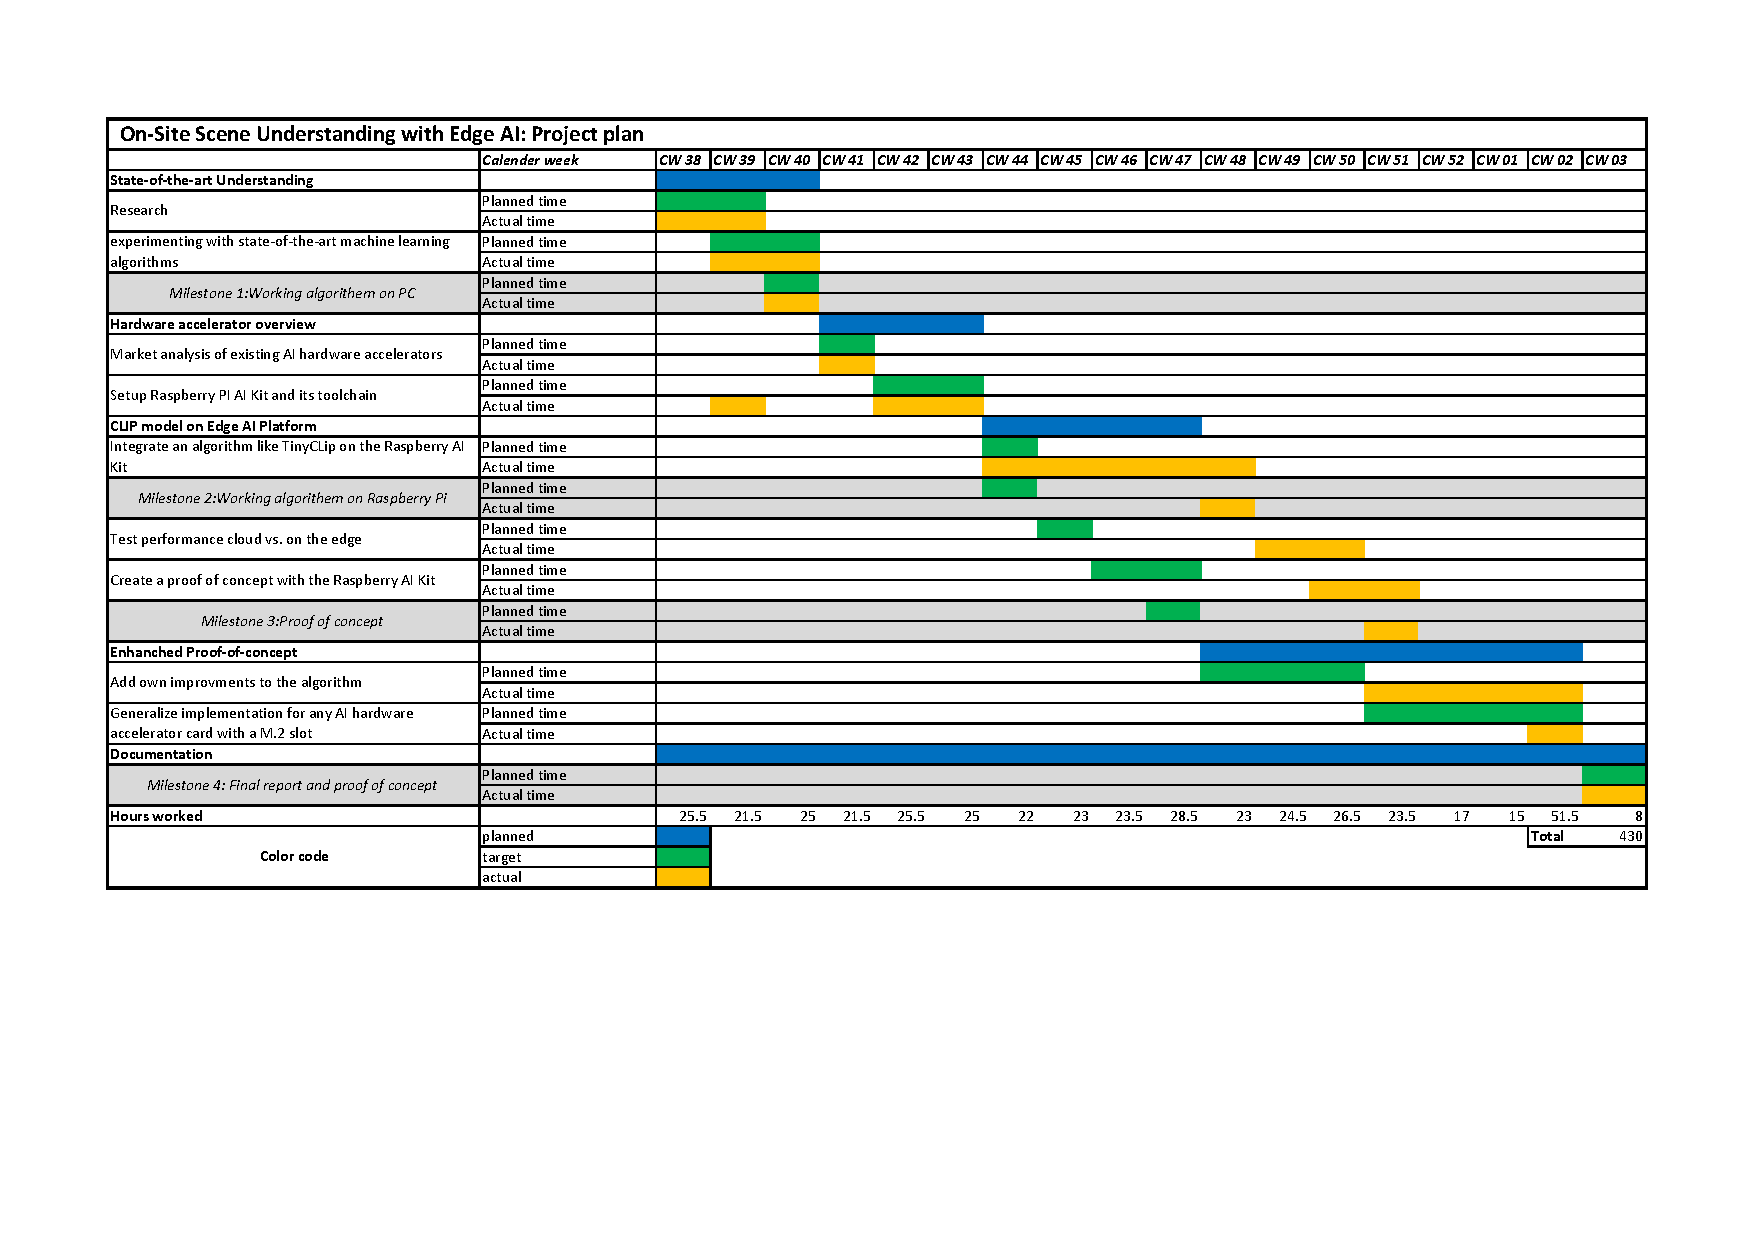
\includegraphics[angle = 90,height = \textheight]{Images/appendix/timetable_Lukas_cut.pdf}
    \caption{timetable}
\end{figure}
    \chapter{Evaluation on PC}
The follow figures are the confusion matricies Evaluation on the respectiv hardware 
\section{With 5 scentens as text embeddings}
\begin{figure}[!h]
    \centering
    \subfloat[][RN50]{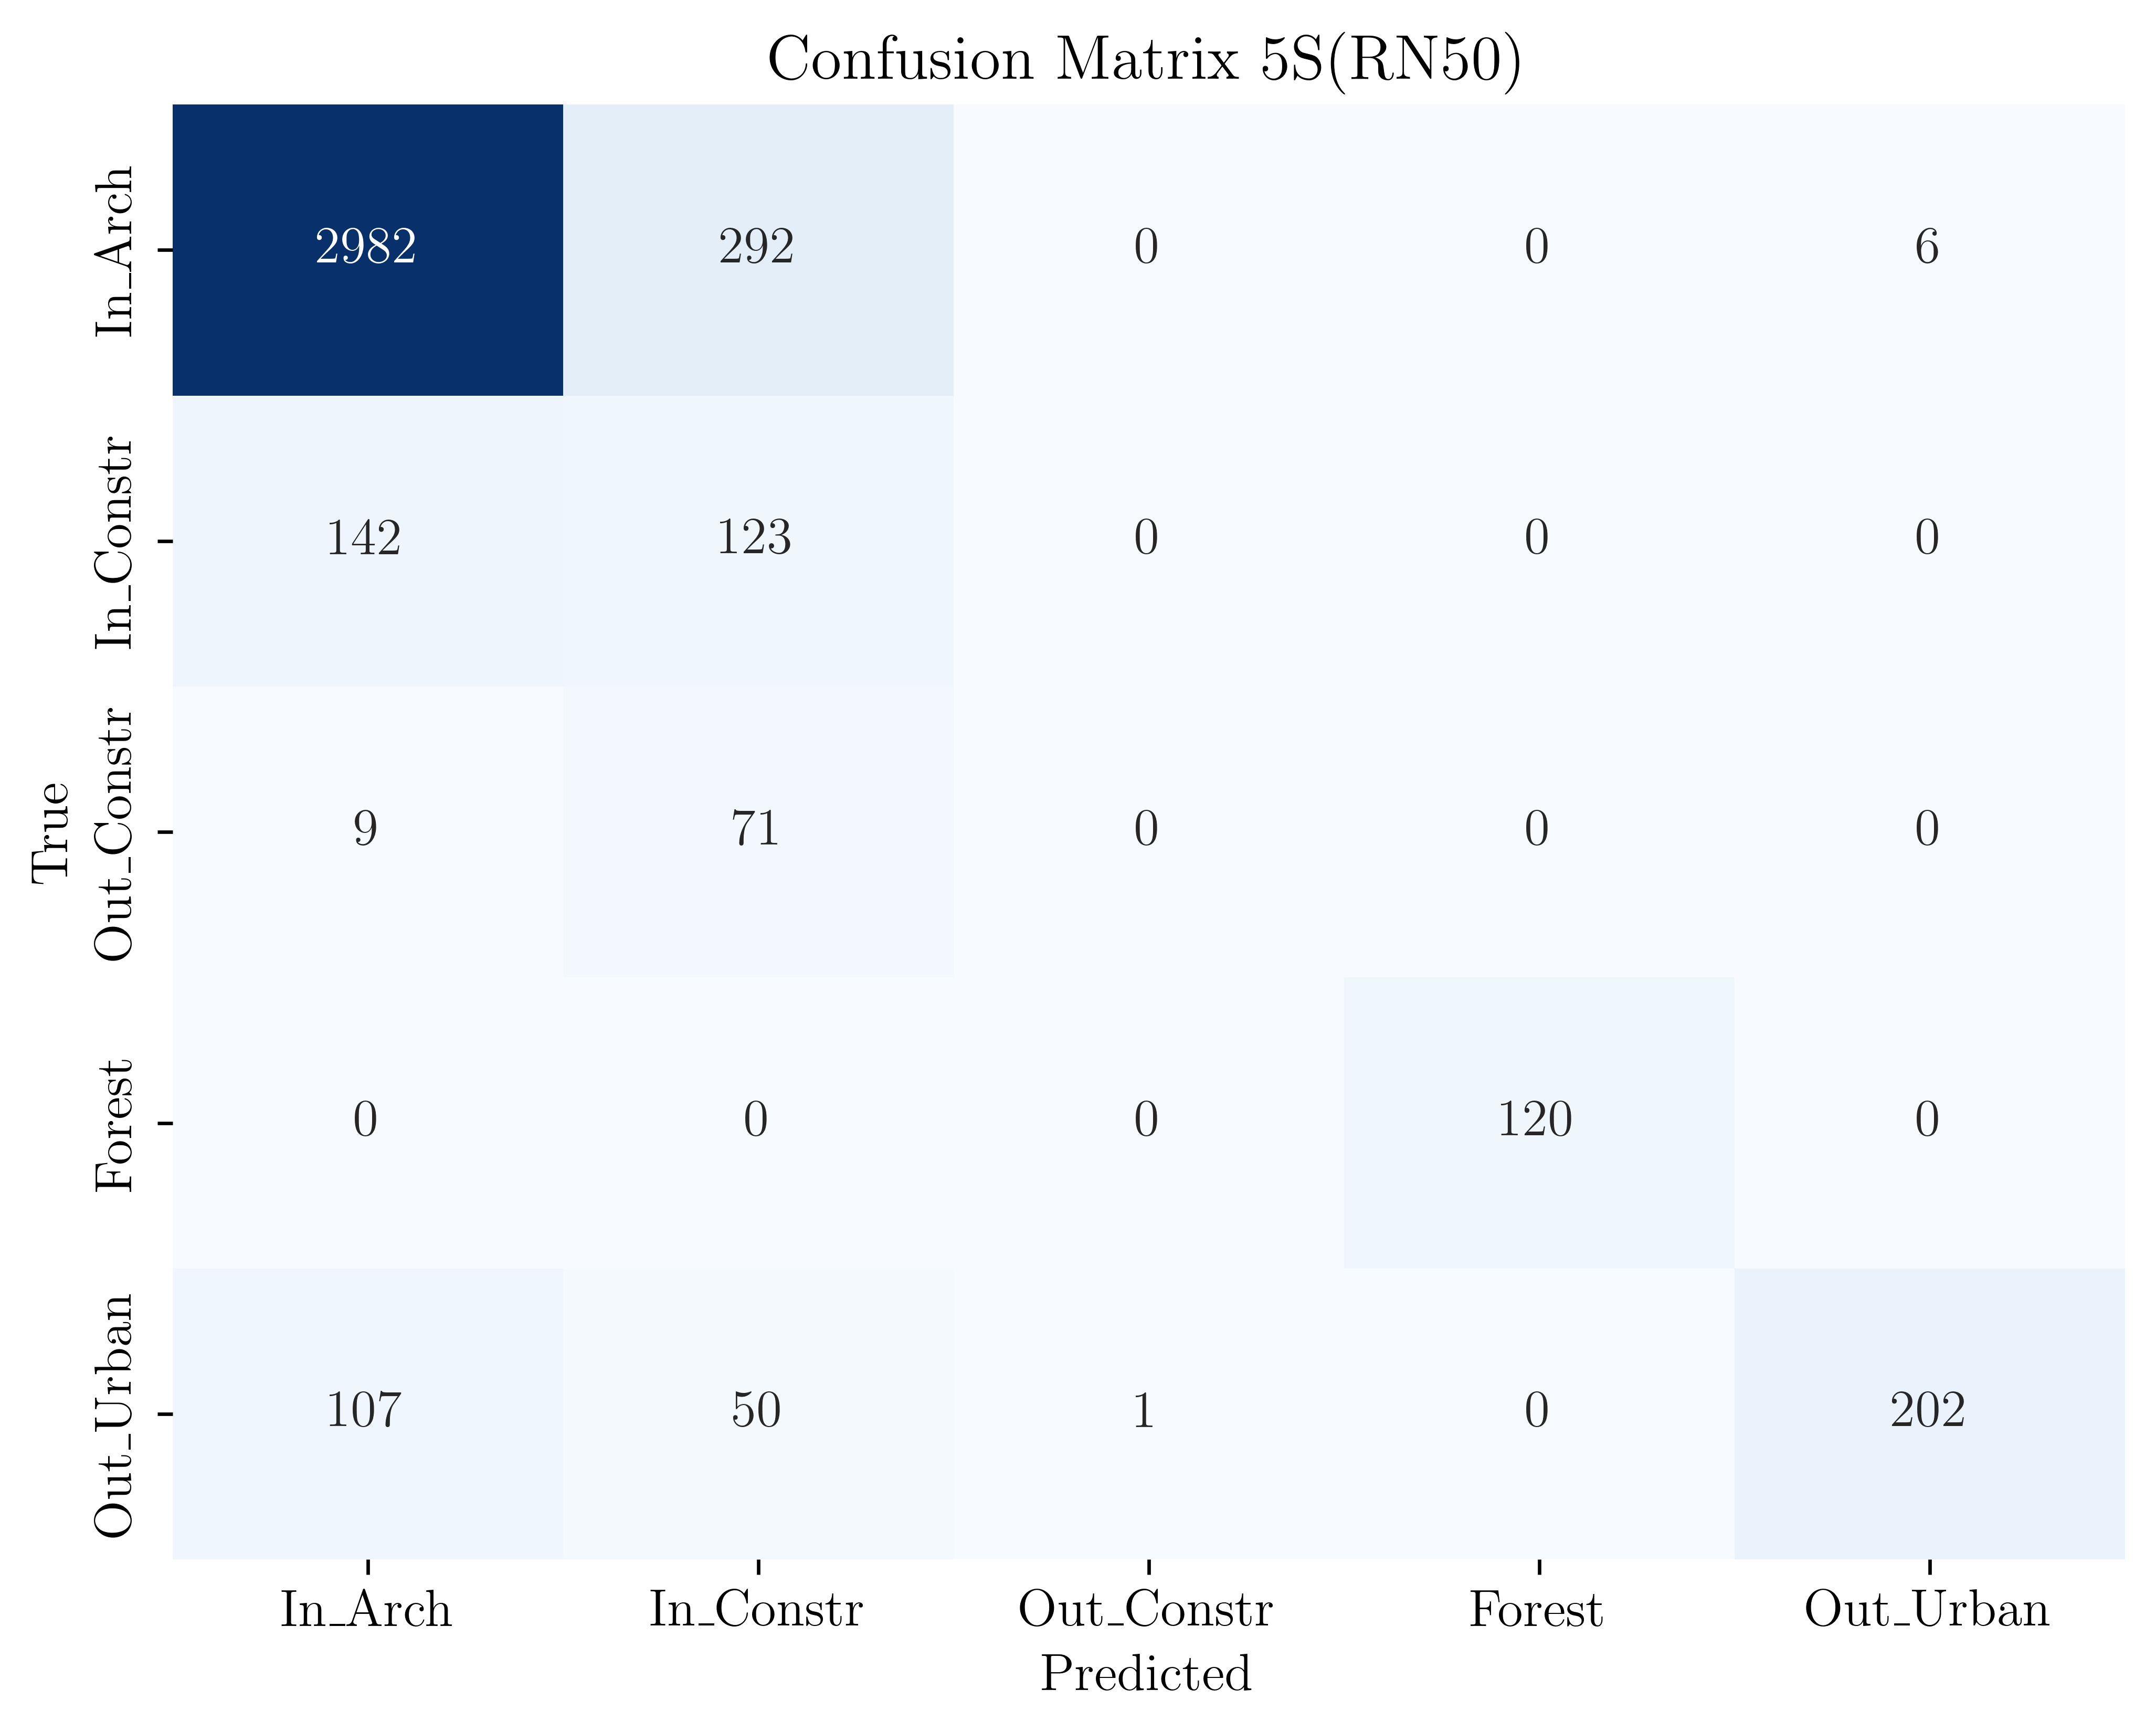
\includegraphics[width=0.49\textwidth]{Images/appendix/resultsPC/Confusion Matrix 5S(RN50).png}\label{resultpc:fig:rn505s}}
    \subfloat[][RN50x4]{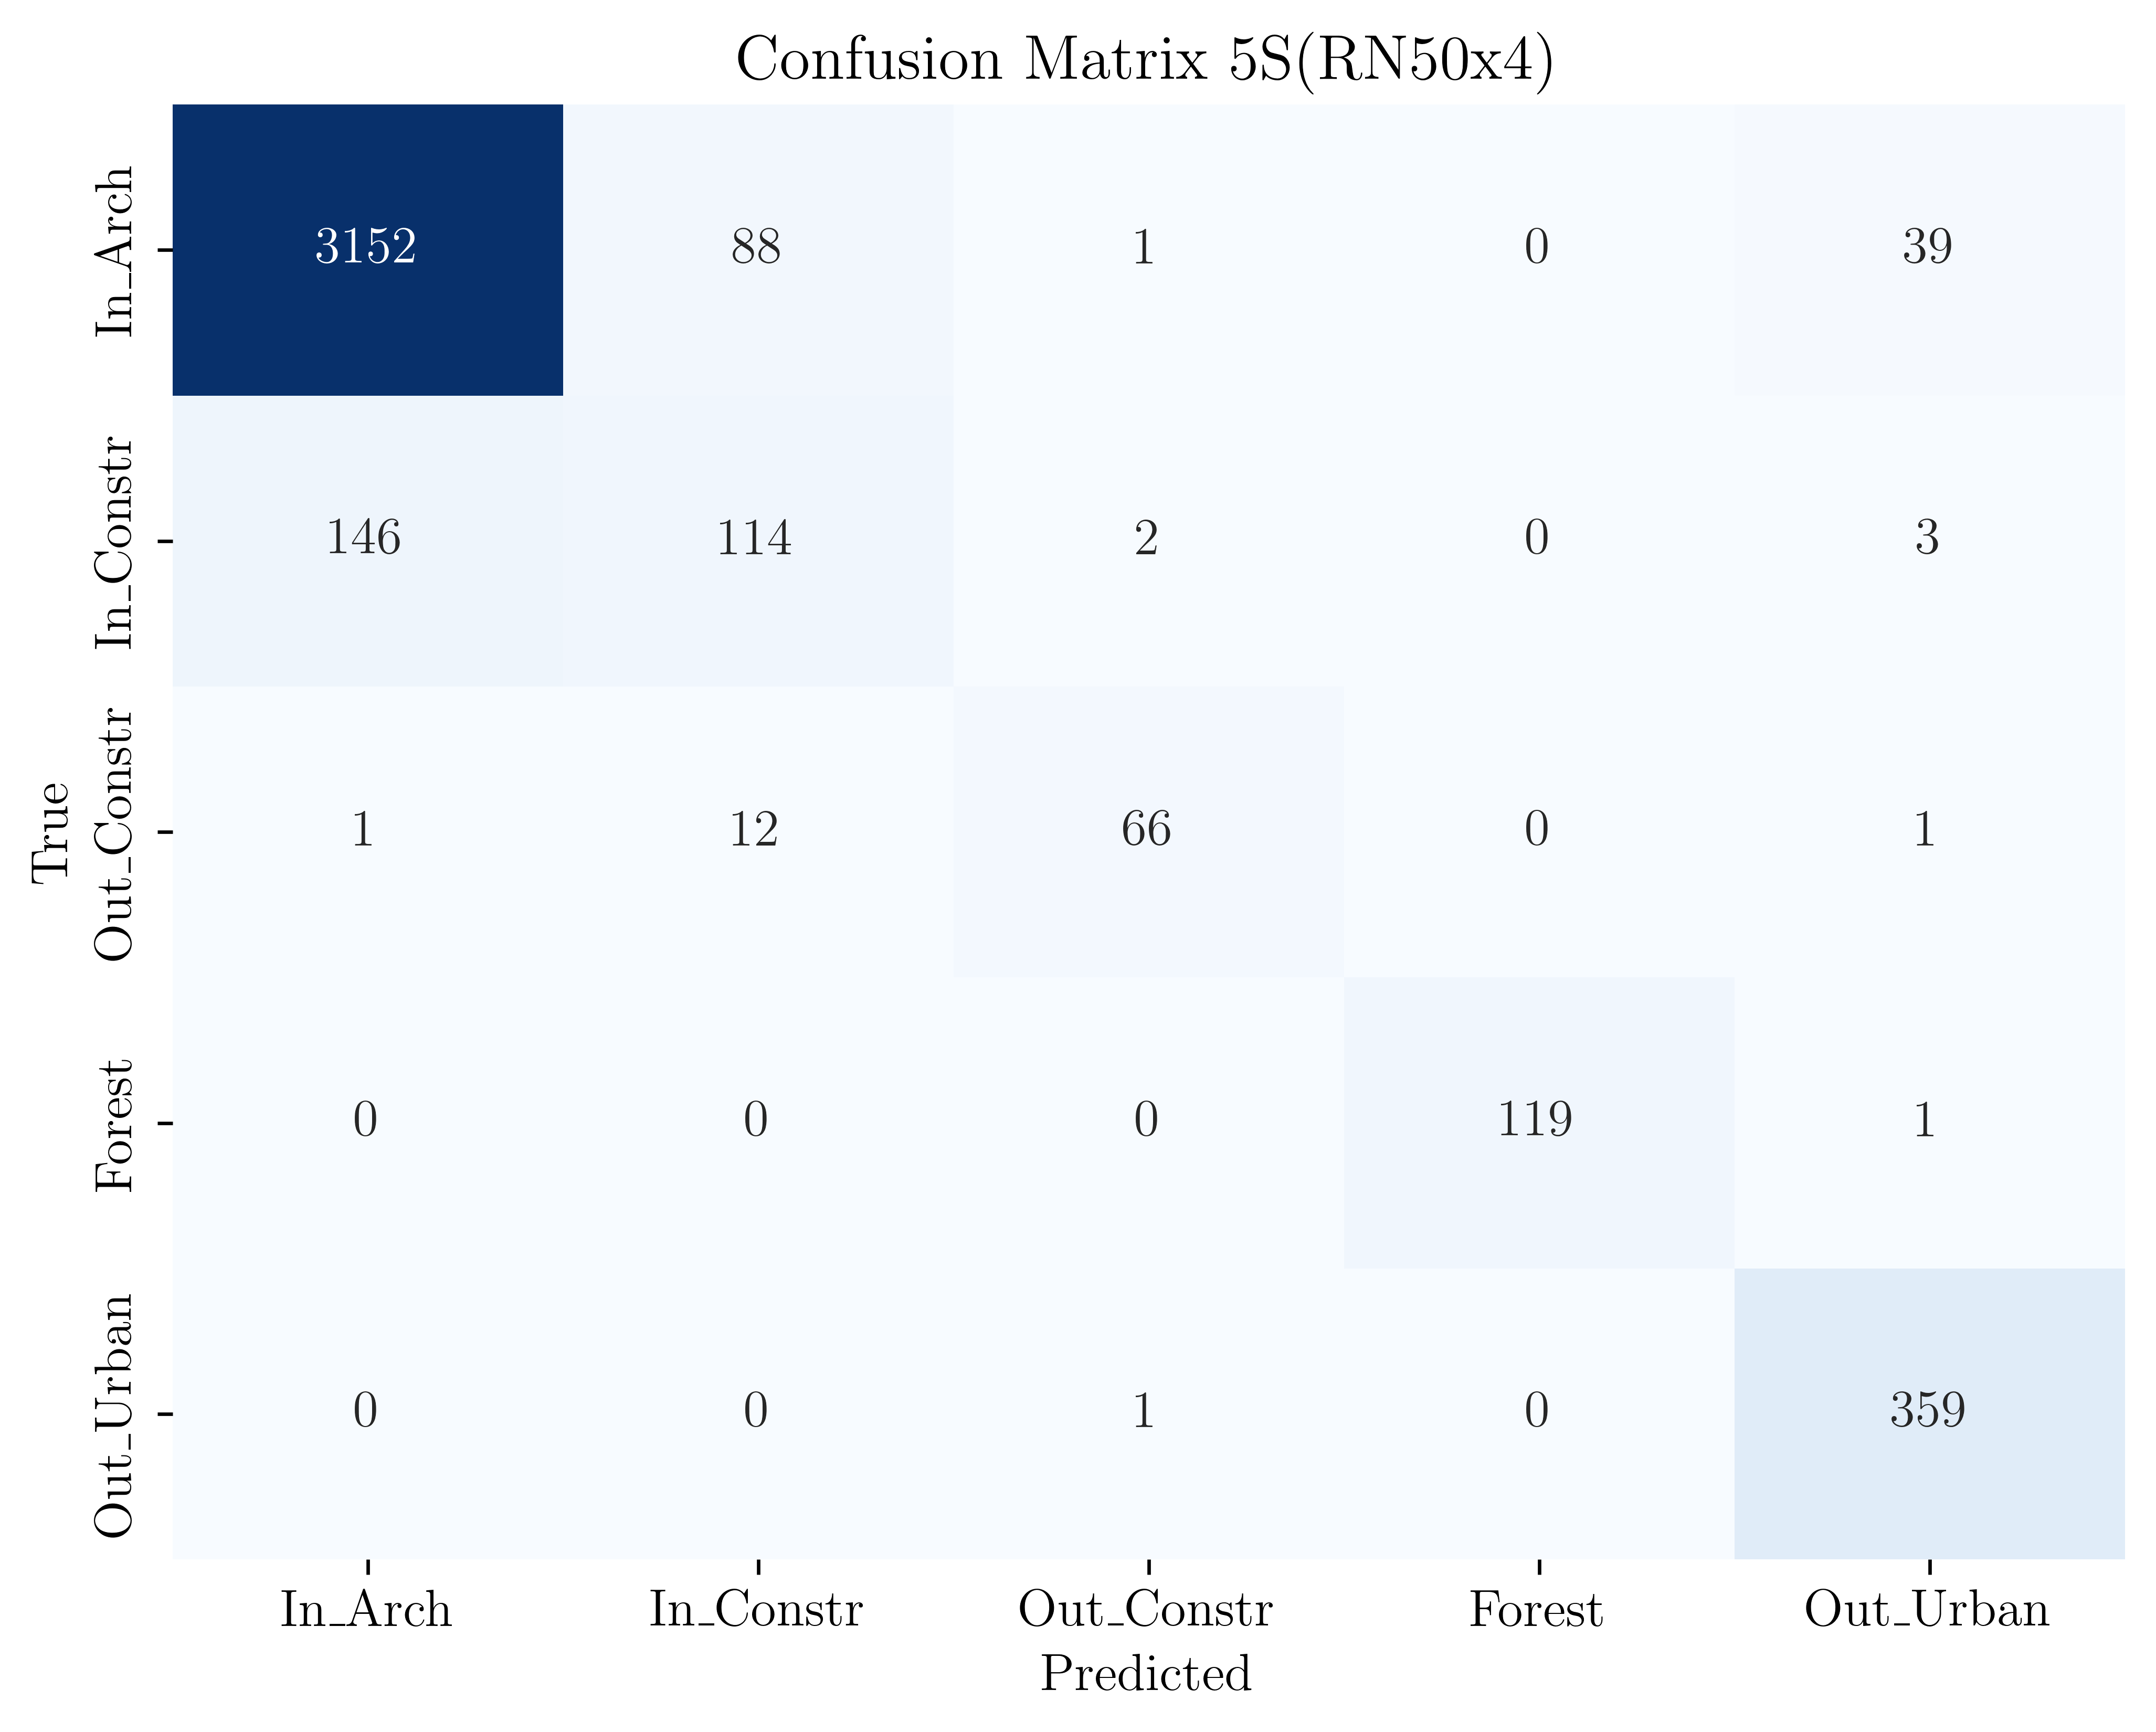
\includegraphics[width=0.49\textwidth]{Images/appendix/resultsPC/Confusion Matrix 5S(RN50x4).png}\label{resultpc:fig:rn50x45s}}
    \quad
    \subfloat[][RN50x16]{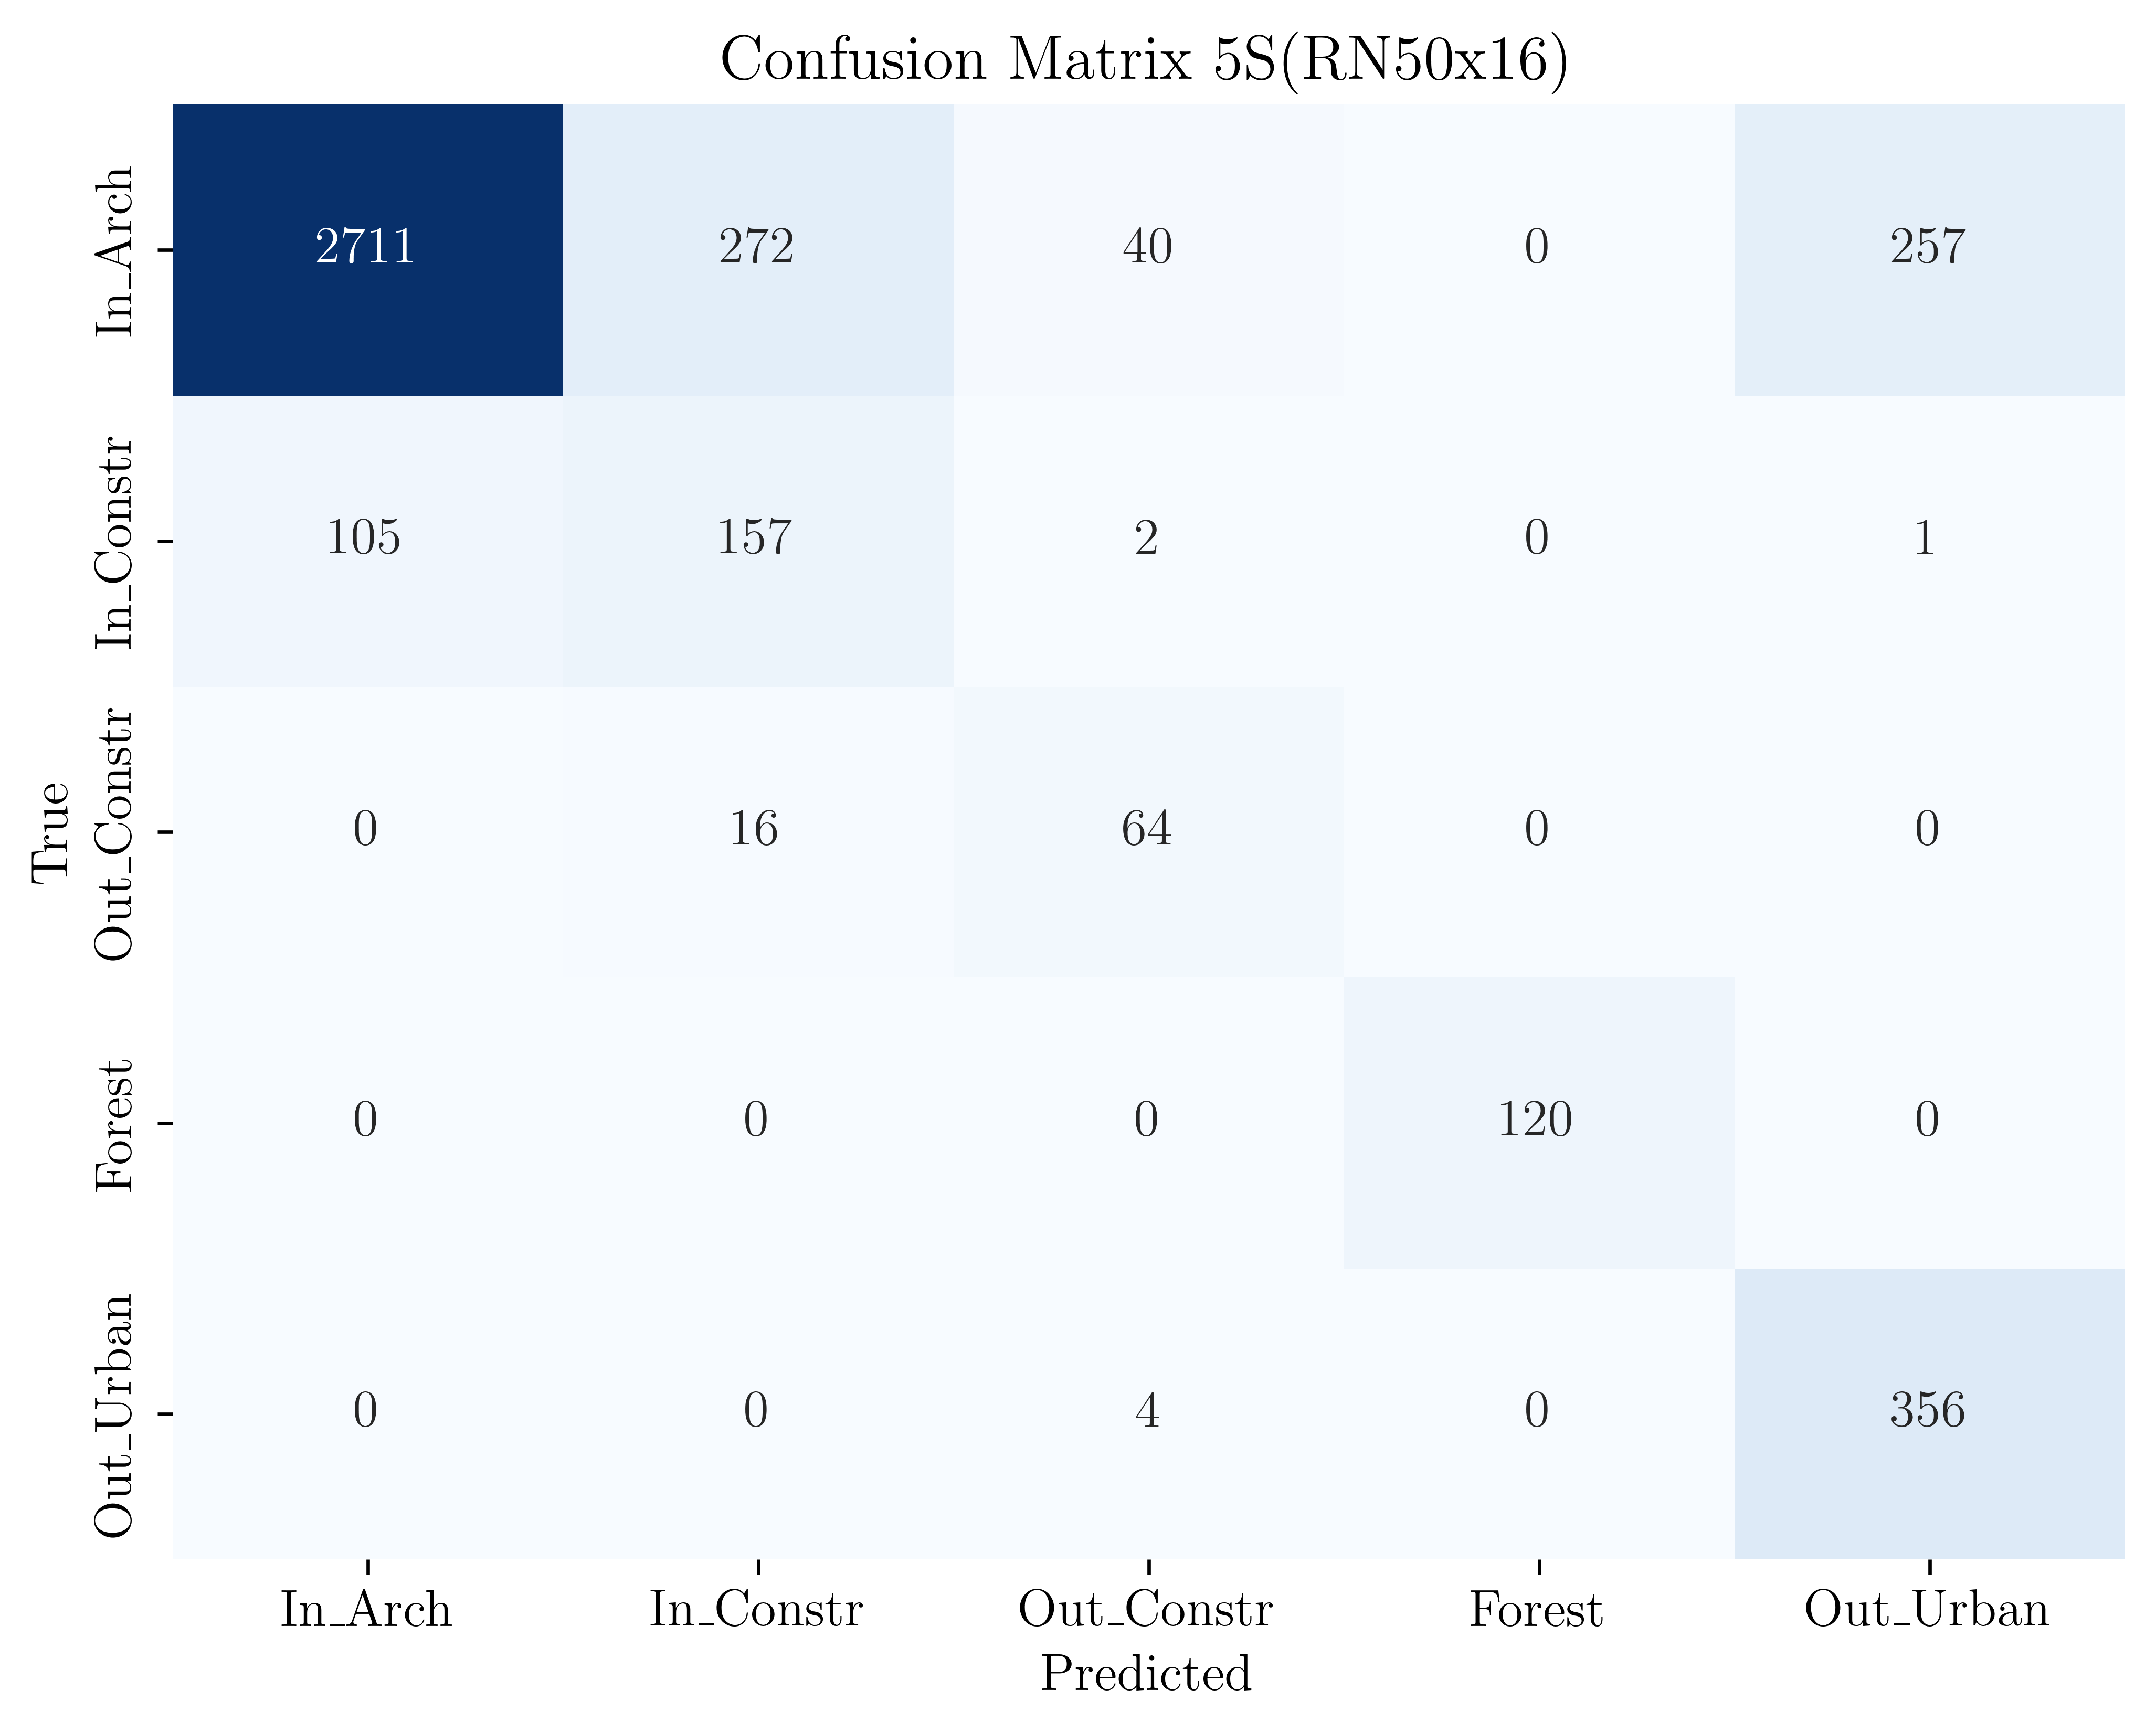
\includegraphics[width=0.49\textwidth]{Images/appendix/resultsPC/Confusion Matrix 5S(RN50x16).png}\label{resultpc:fig:rn50x165s}}
    \subfloat[][RN50x64]{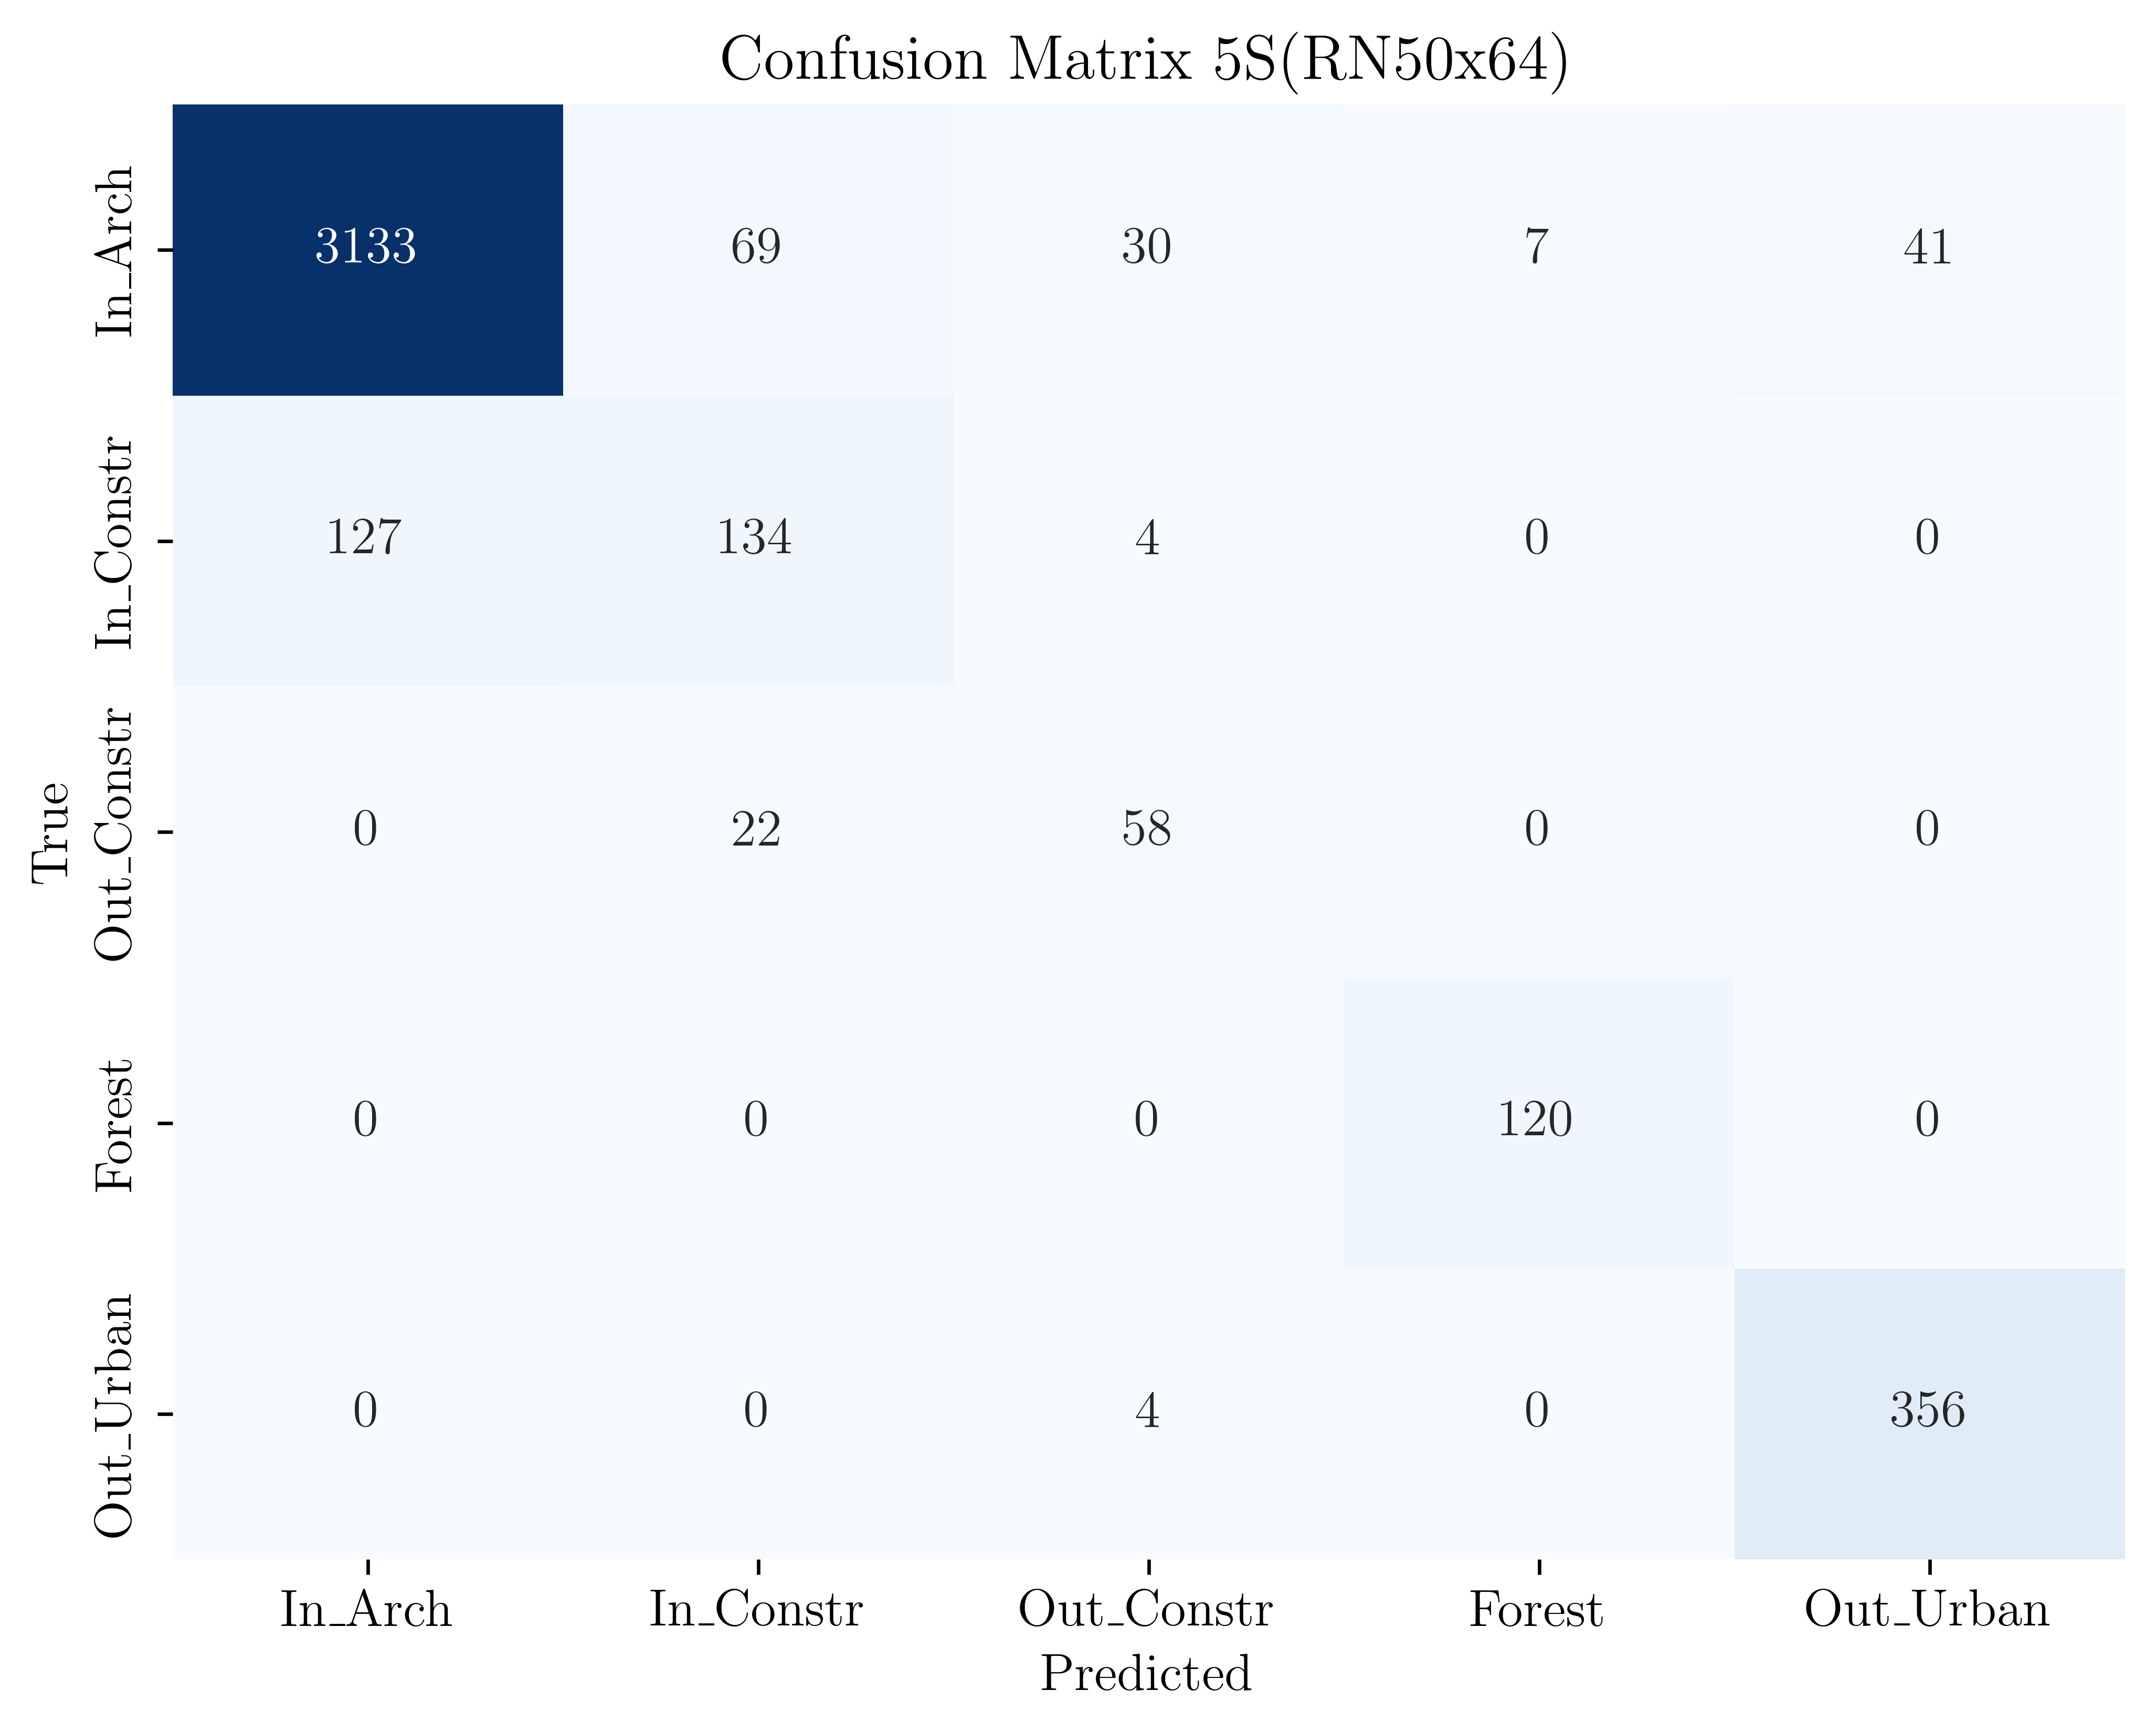
\includegraphics[width=0.49\textwidth]{Images/appendix/resultsPC/Confusion Matrix 5S(RN50x64).png}\label{resultpc:fig:rn50x645s}}
   
\end{figure}

\begin{figure}
    %\ContinuedFloat
    \centering
    \subfloat[][RN101]{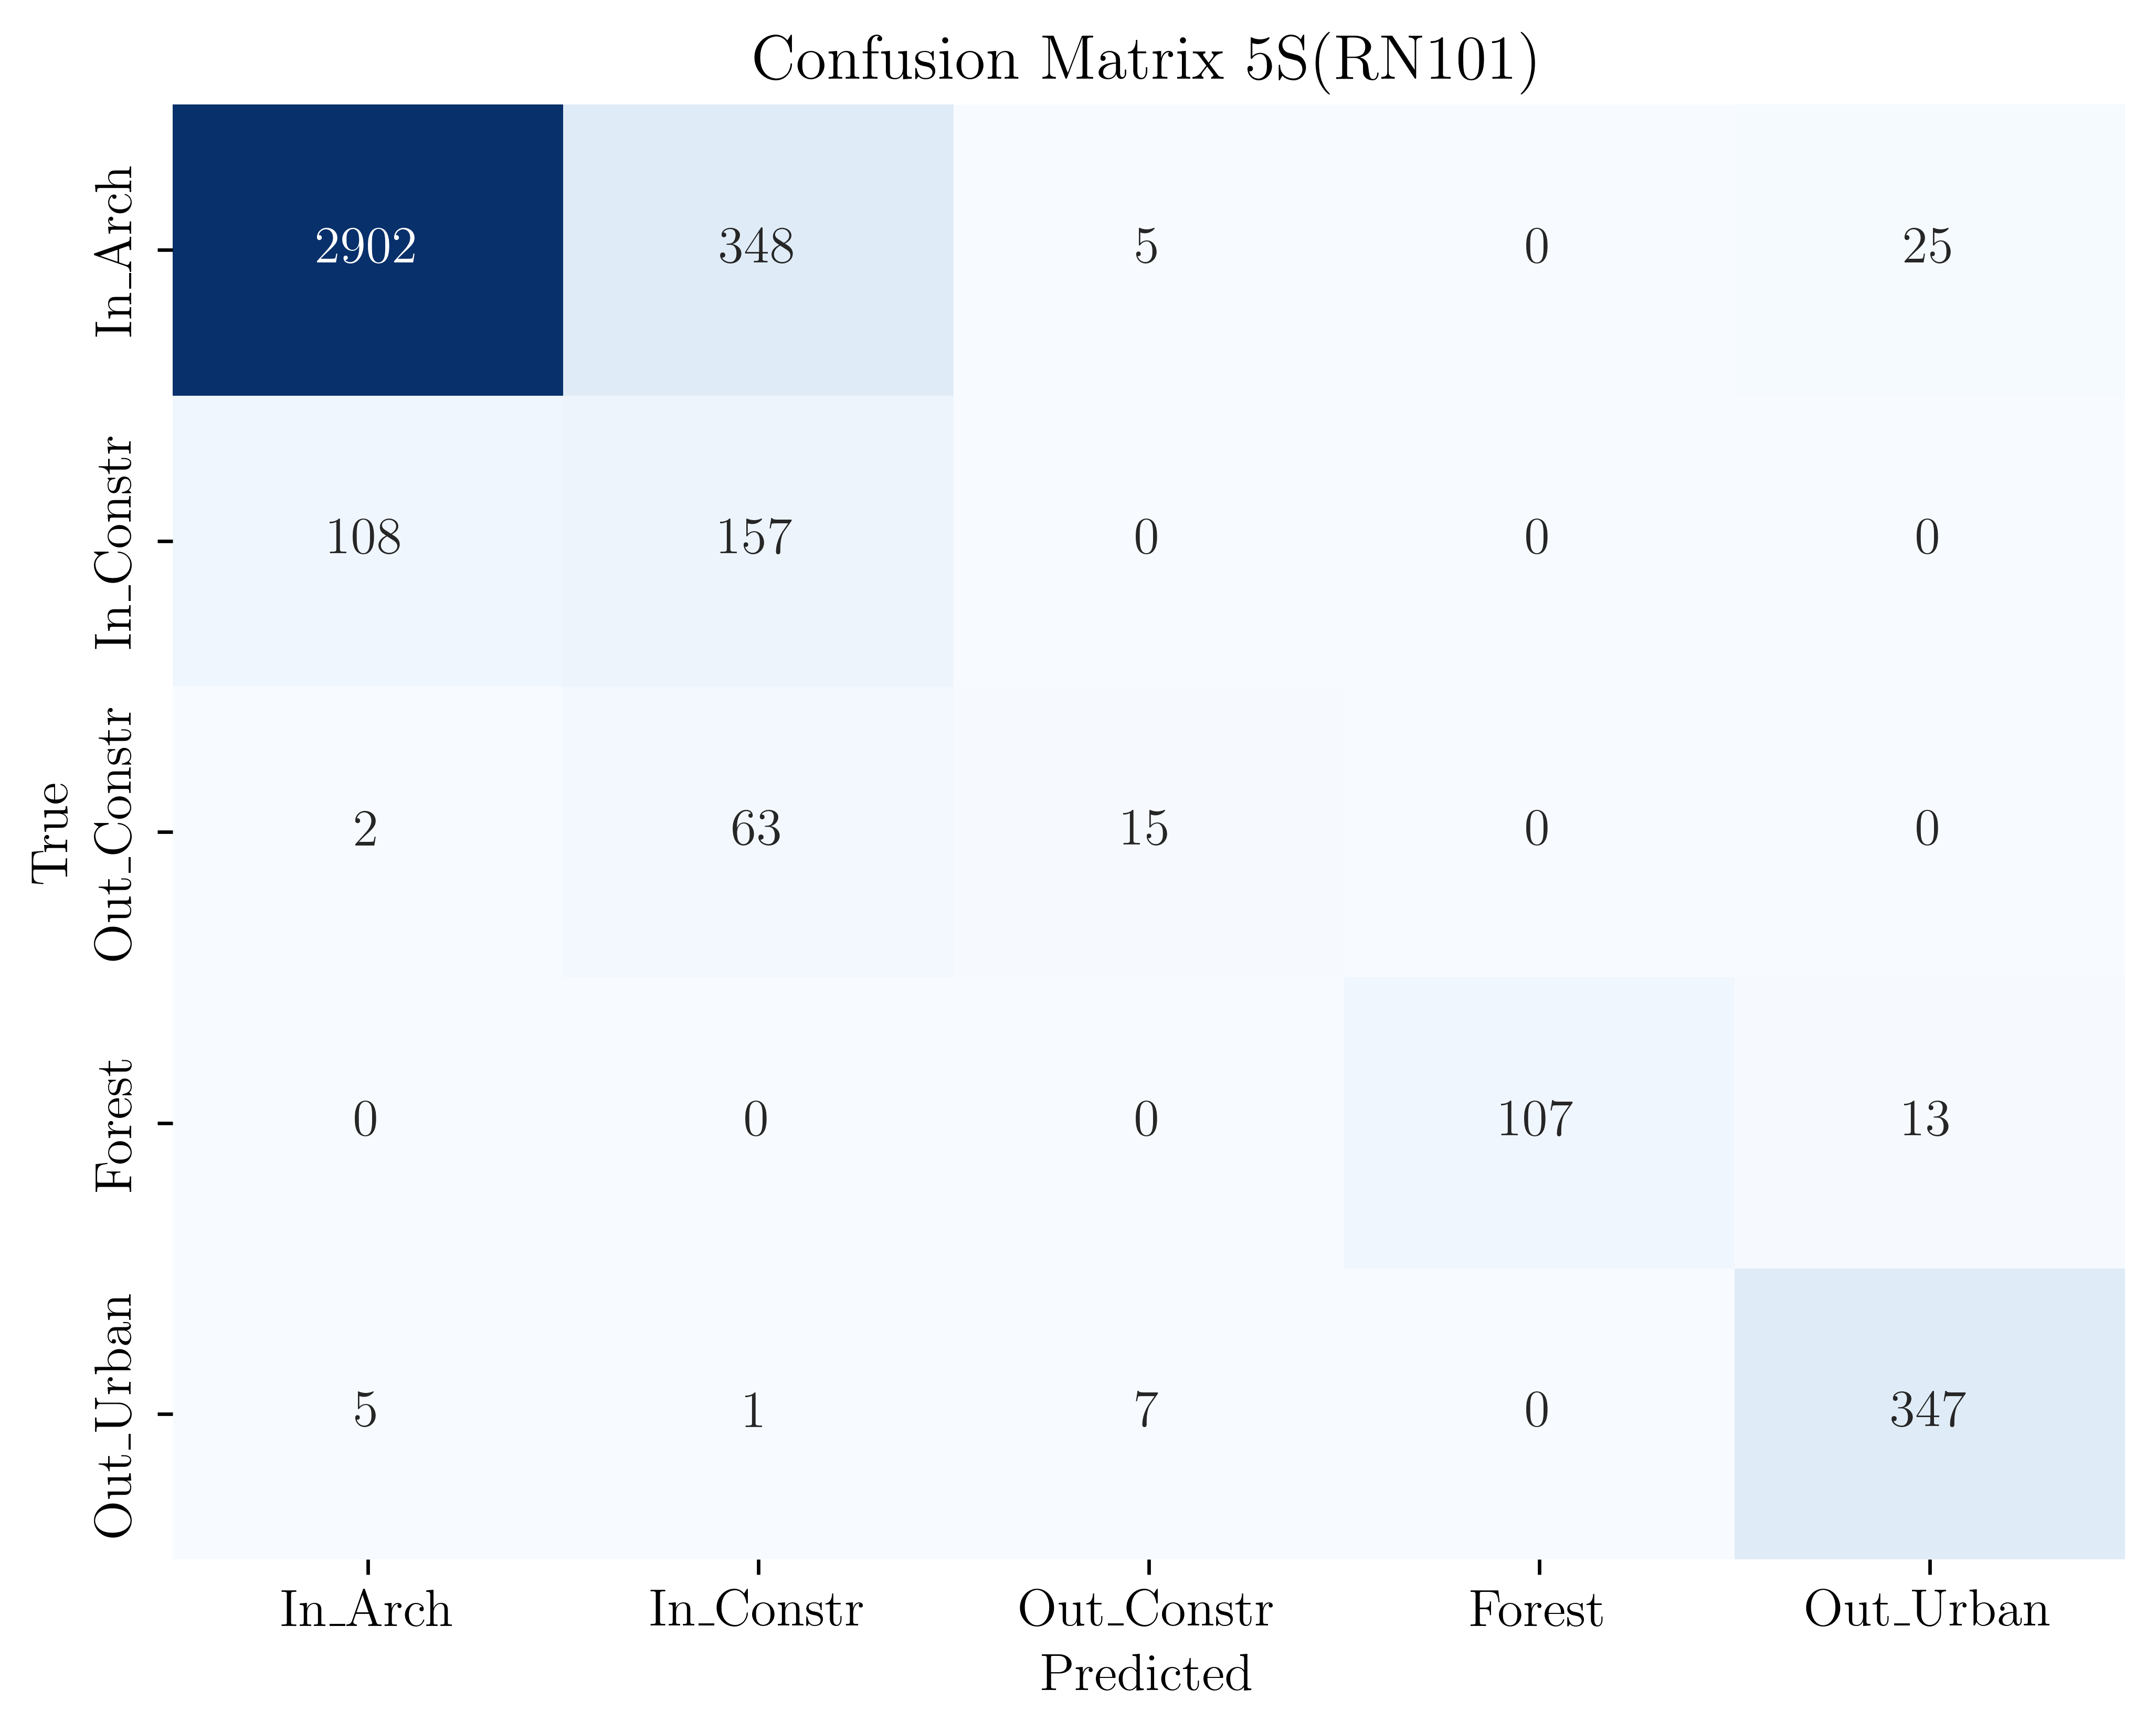
\includegraphics[width=0.49\textwidth]{Images/appendix/resultsPC/Confusion Matrix 5S(RN101).png}\label{resultpc:fig:rn1015s}}
    \subfloat[][TinyCLIP 19M]{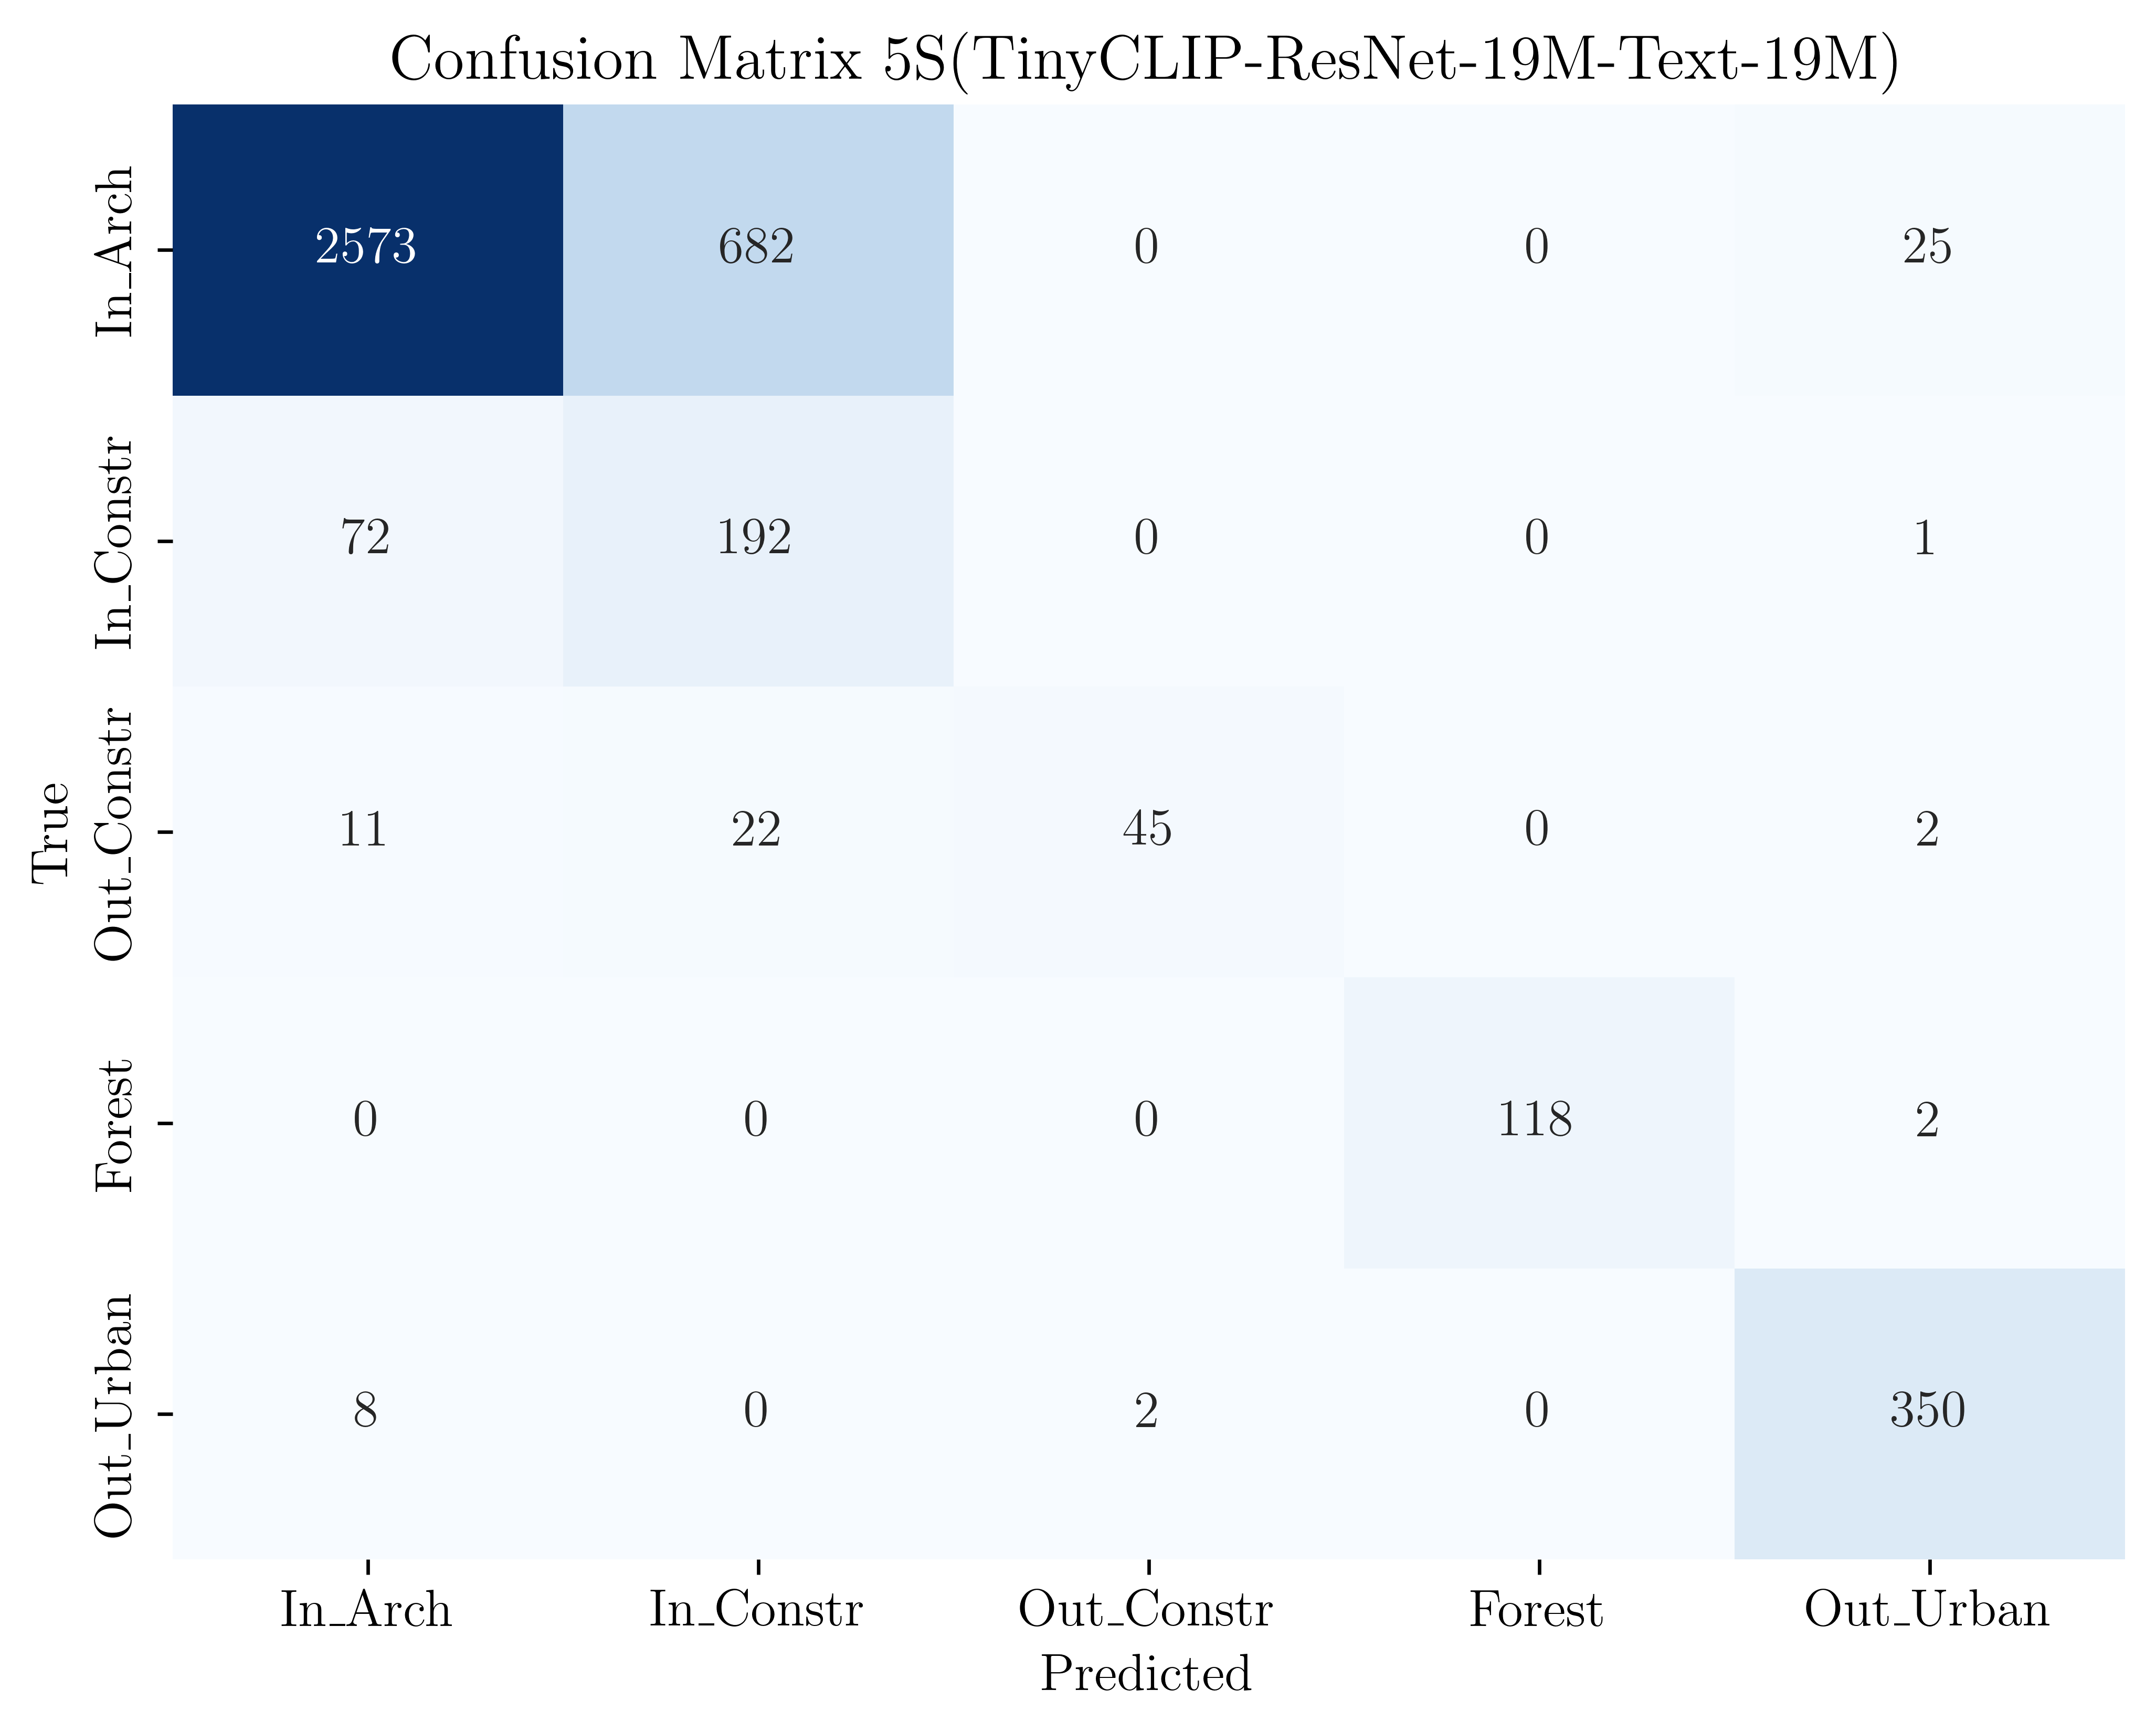
\includegraphics[width=0.49\textwidth]{Images/appendix/resultsPC/Confusion Matrix 5S(TinyCLIP-ResNet-19M-Text-19M).png}\label{resultpc:fig:tiny195s}}
    \quad
    \subfloat[][TinyCLIP 30M]{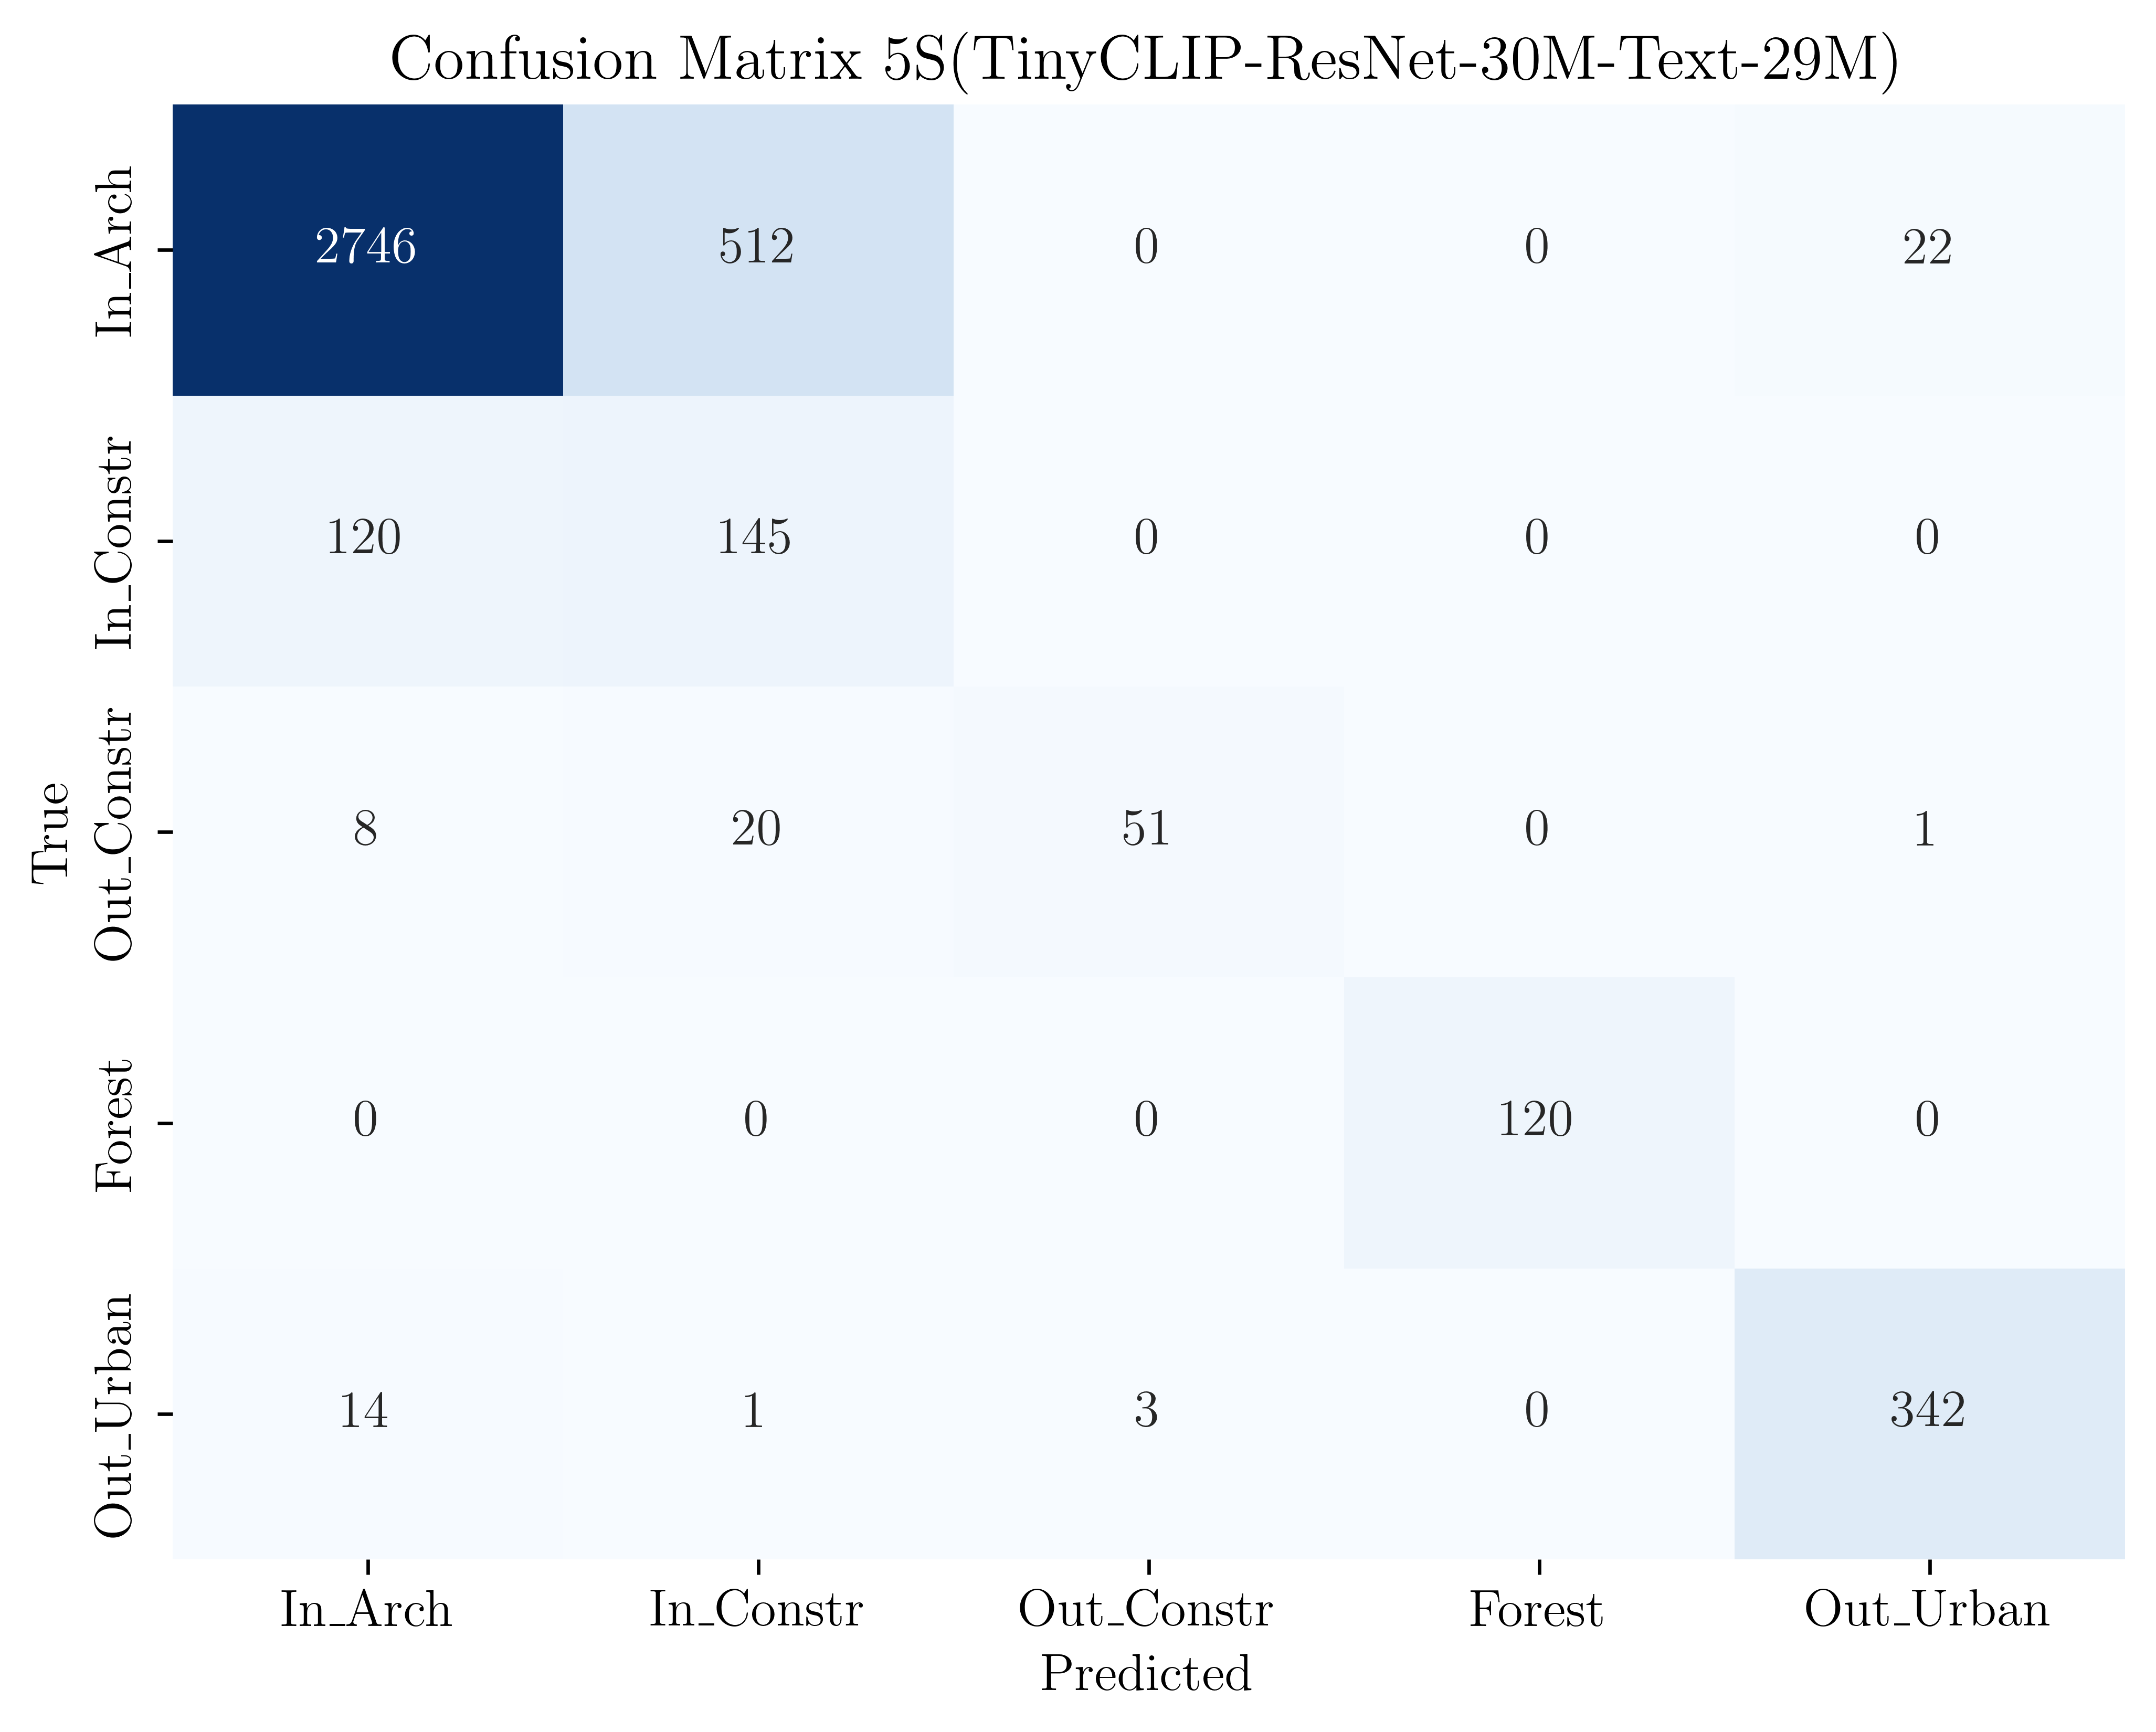
\includegraphics[width=0.49\textwidth]{Images/appendix/resultsPC/Confusion Matrix 5S(TinyCLIP-ResNet-30M-Text-29M).png}\label{resultpc:fig:tiny305s}}
    \caption{Confusion matrix on PC with 5 scentens as text embeddings}
    \label{resultpc:fig:evalpc5s}
\end{figure}

\section{With pure text prompts as text embeddings}
\begin{figure}[!ht]
    \centering
    \subfloat[][RN50]{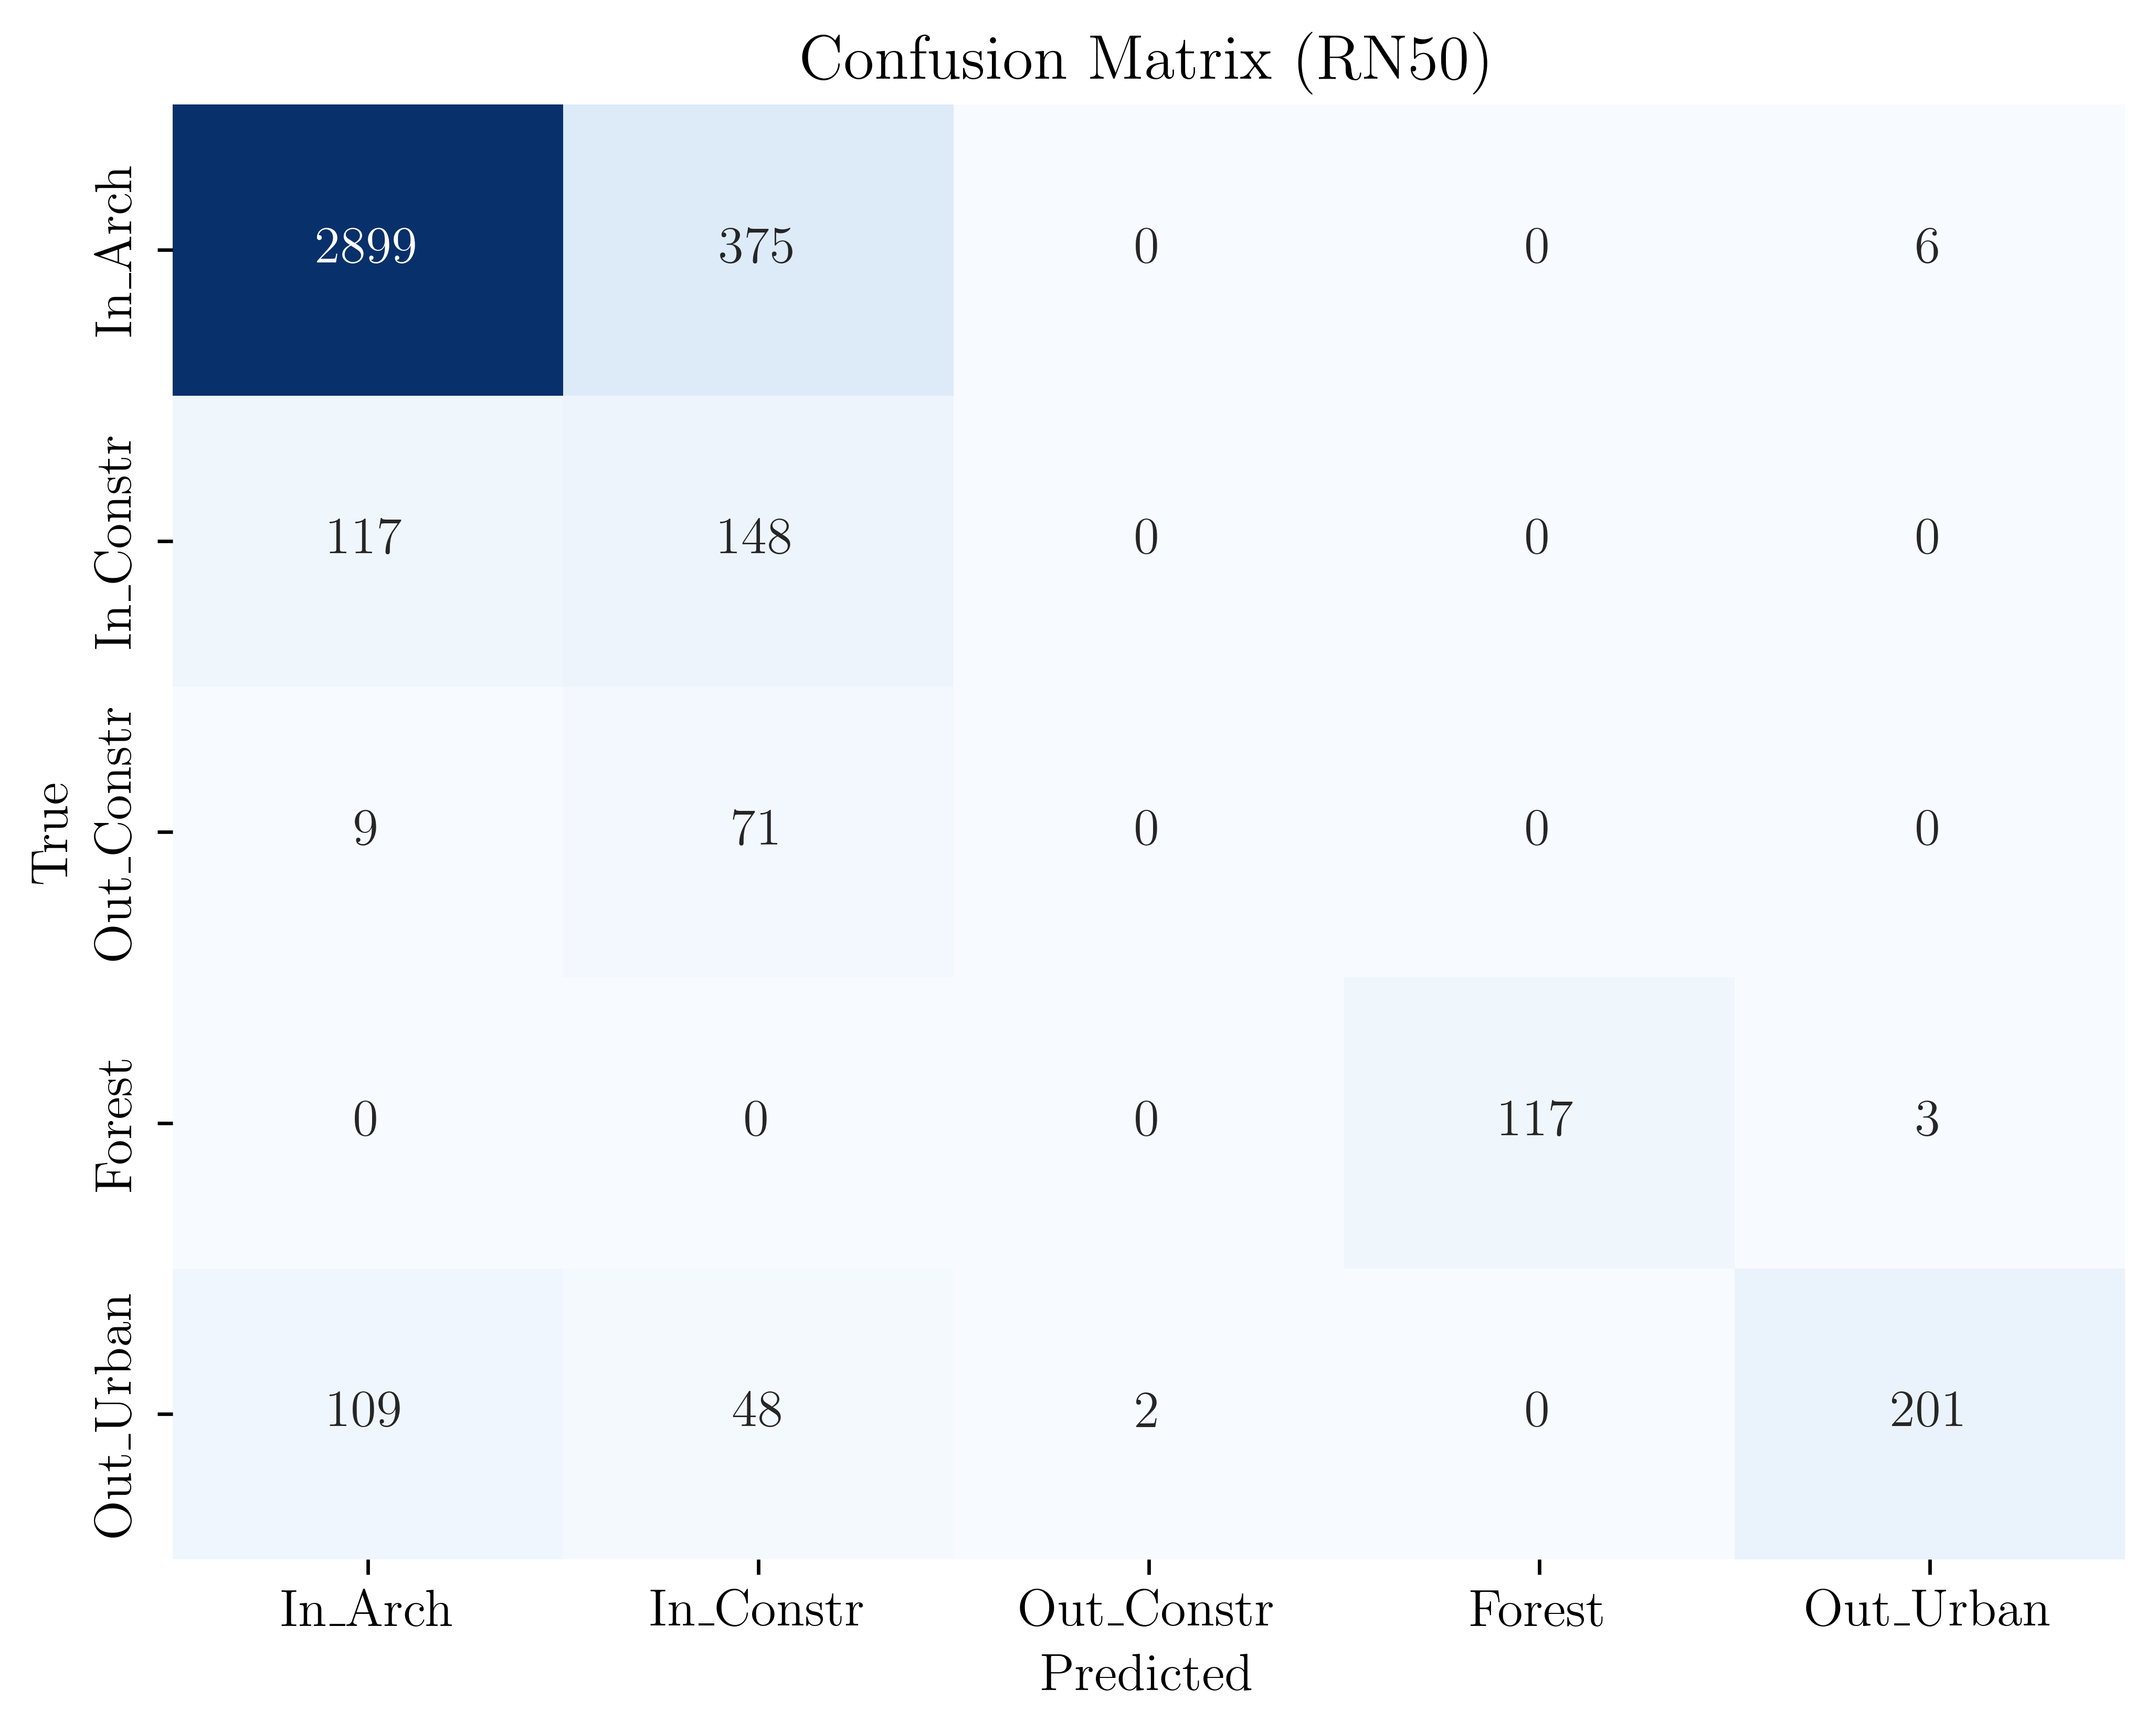
\includegraphics[width=0.49\textwidth]{Images/appendix/resultsPC/Confusion Matrix (RN50).png}\label{resultpc:fig:rn50}}
    \subfloat[][RN50x4]{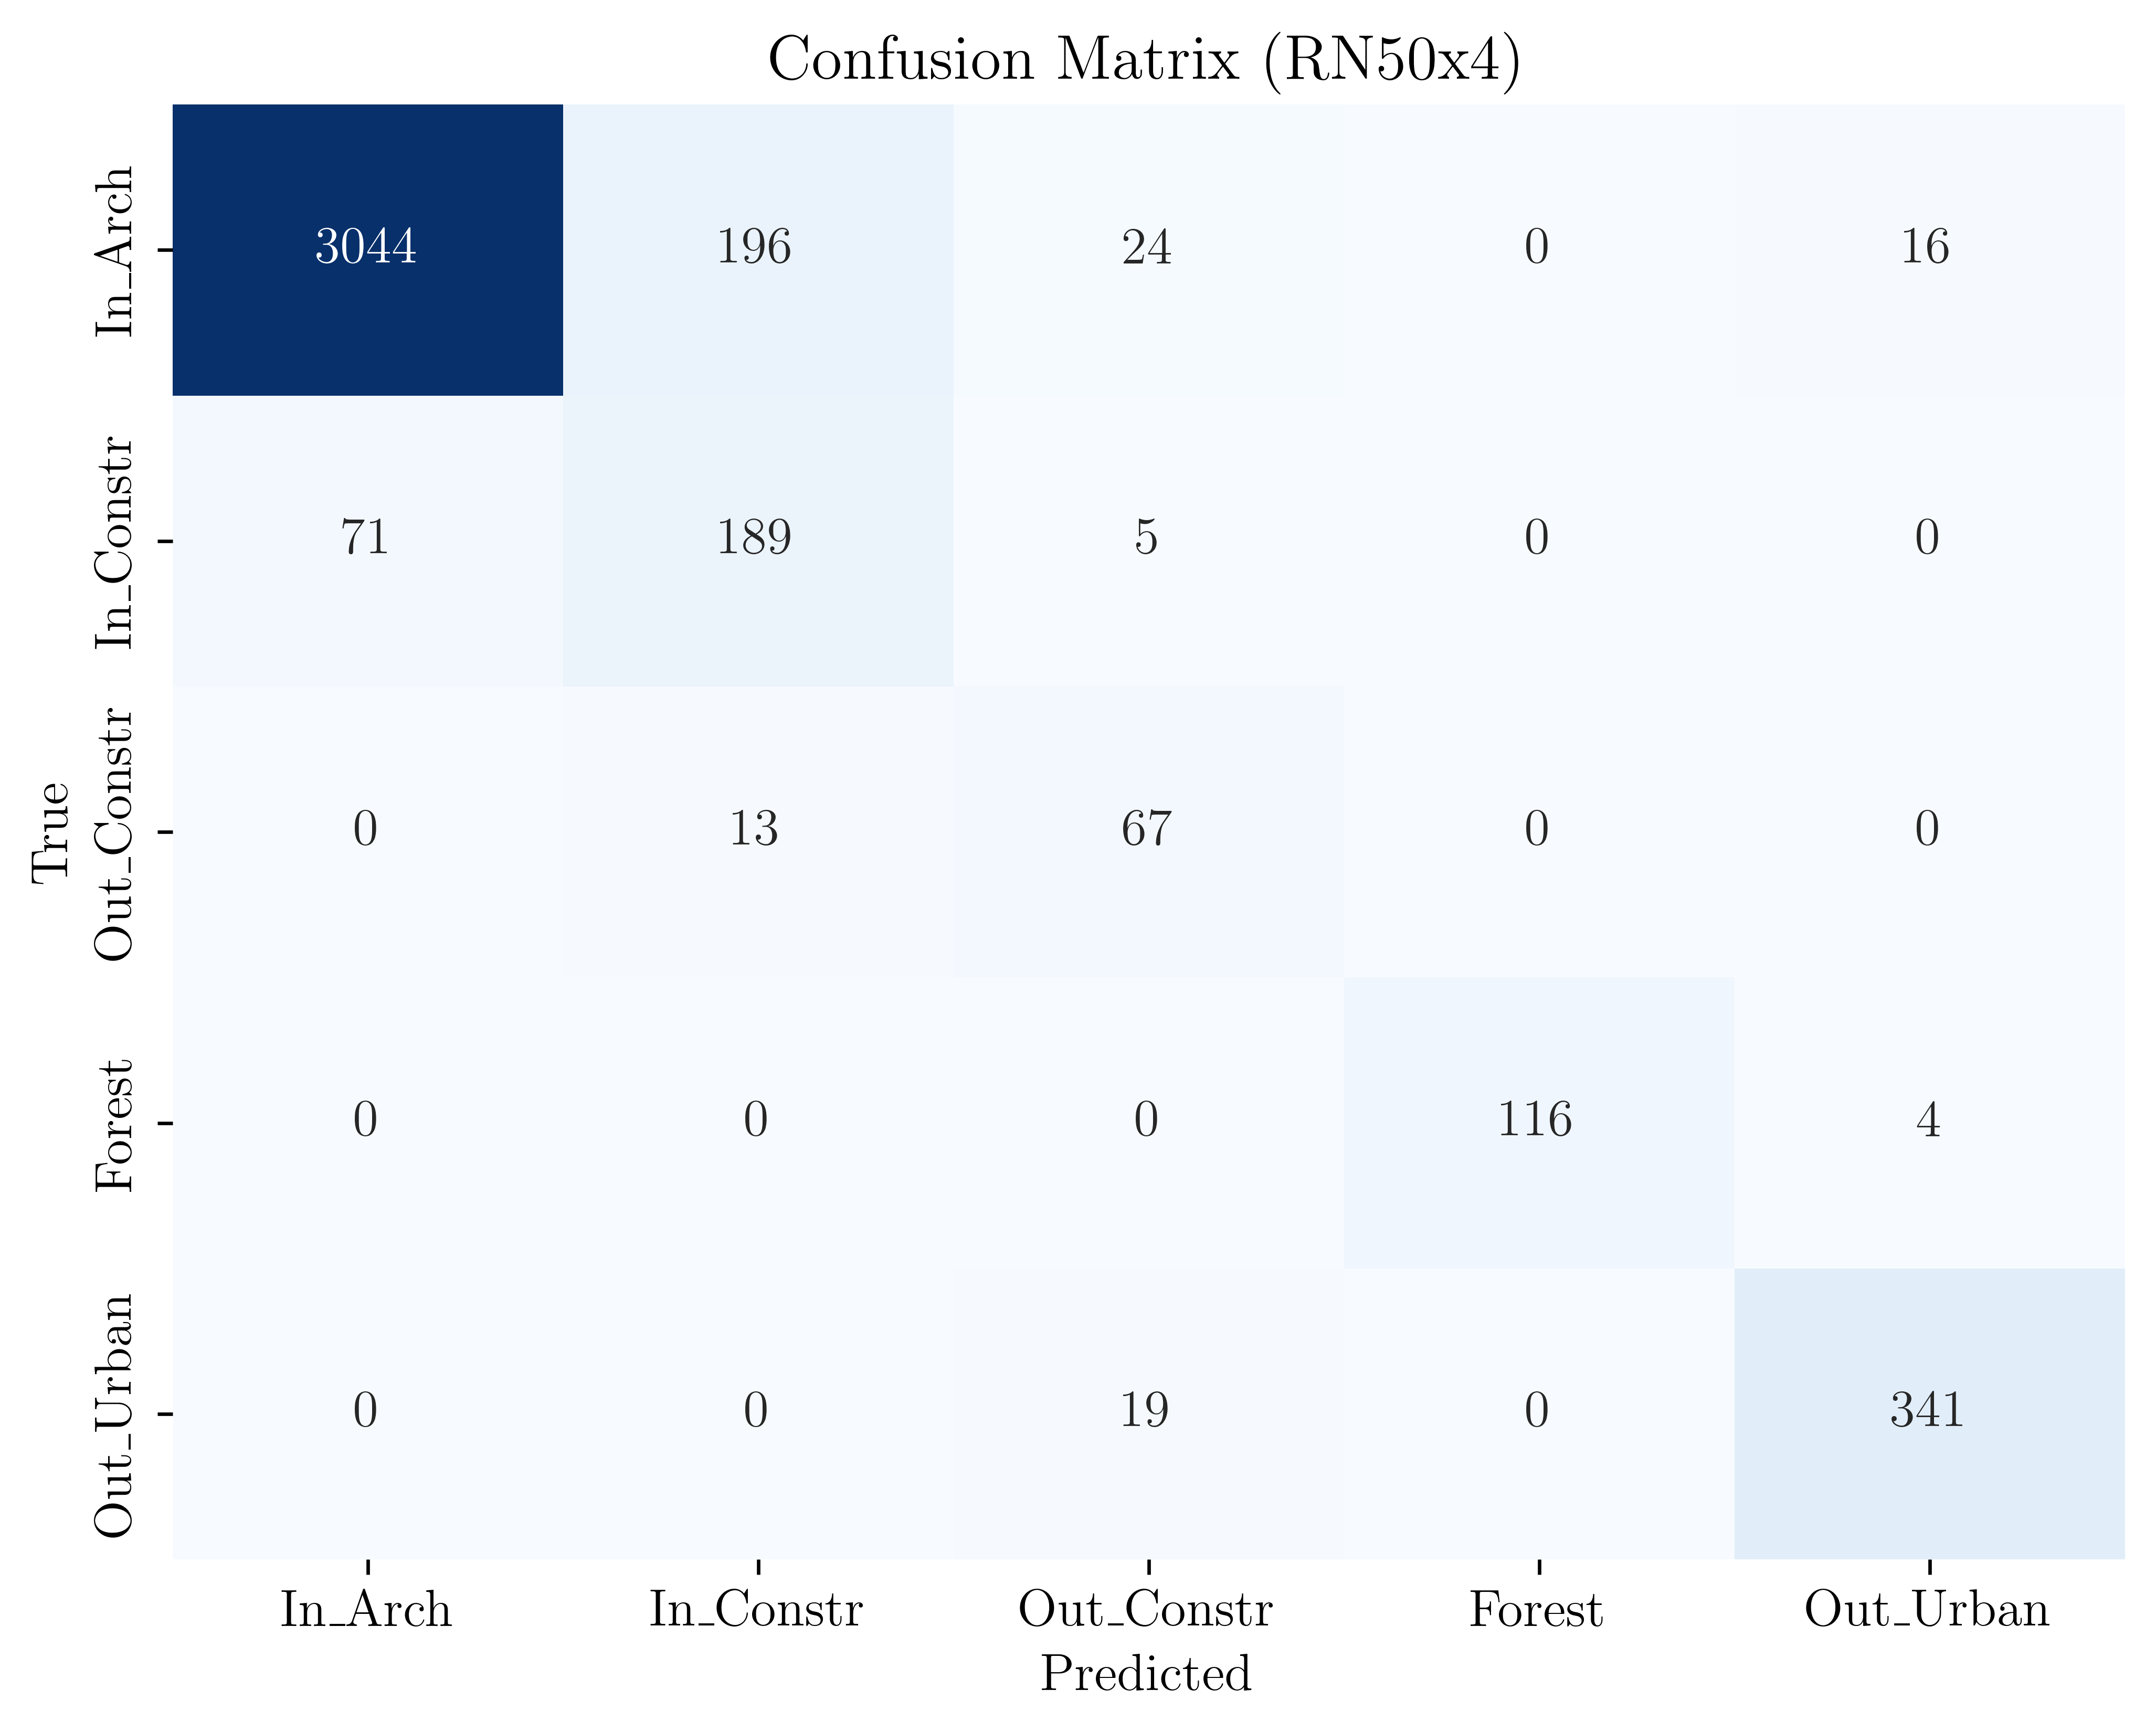
\includegraphics[width=0.49\textwidth]{Images/appendix/resultsPC/Confusion Matrix (RN50x4).png}\label{resultpc:fig:rn50x4}}
    \quad
    \subfloat[][RN50x16]{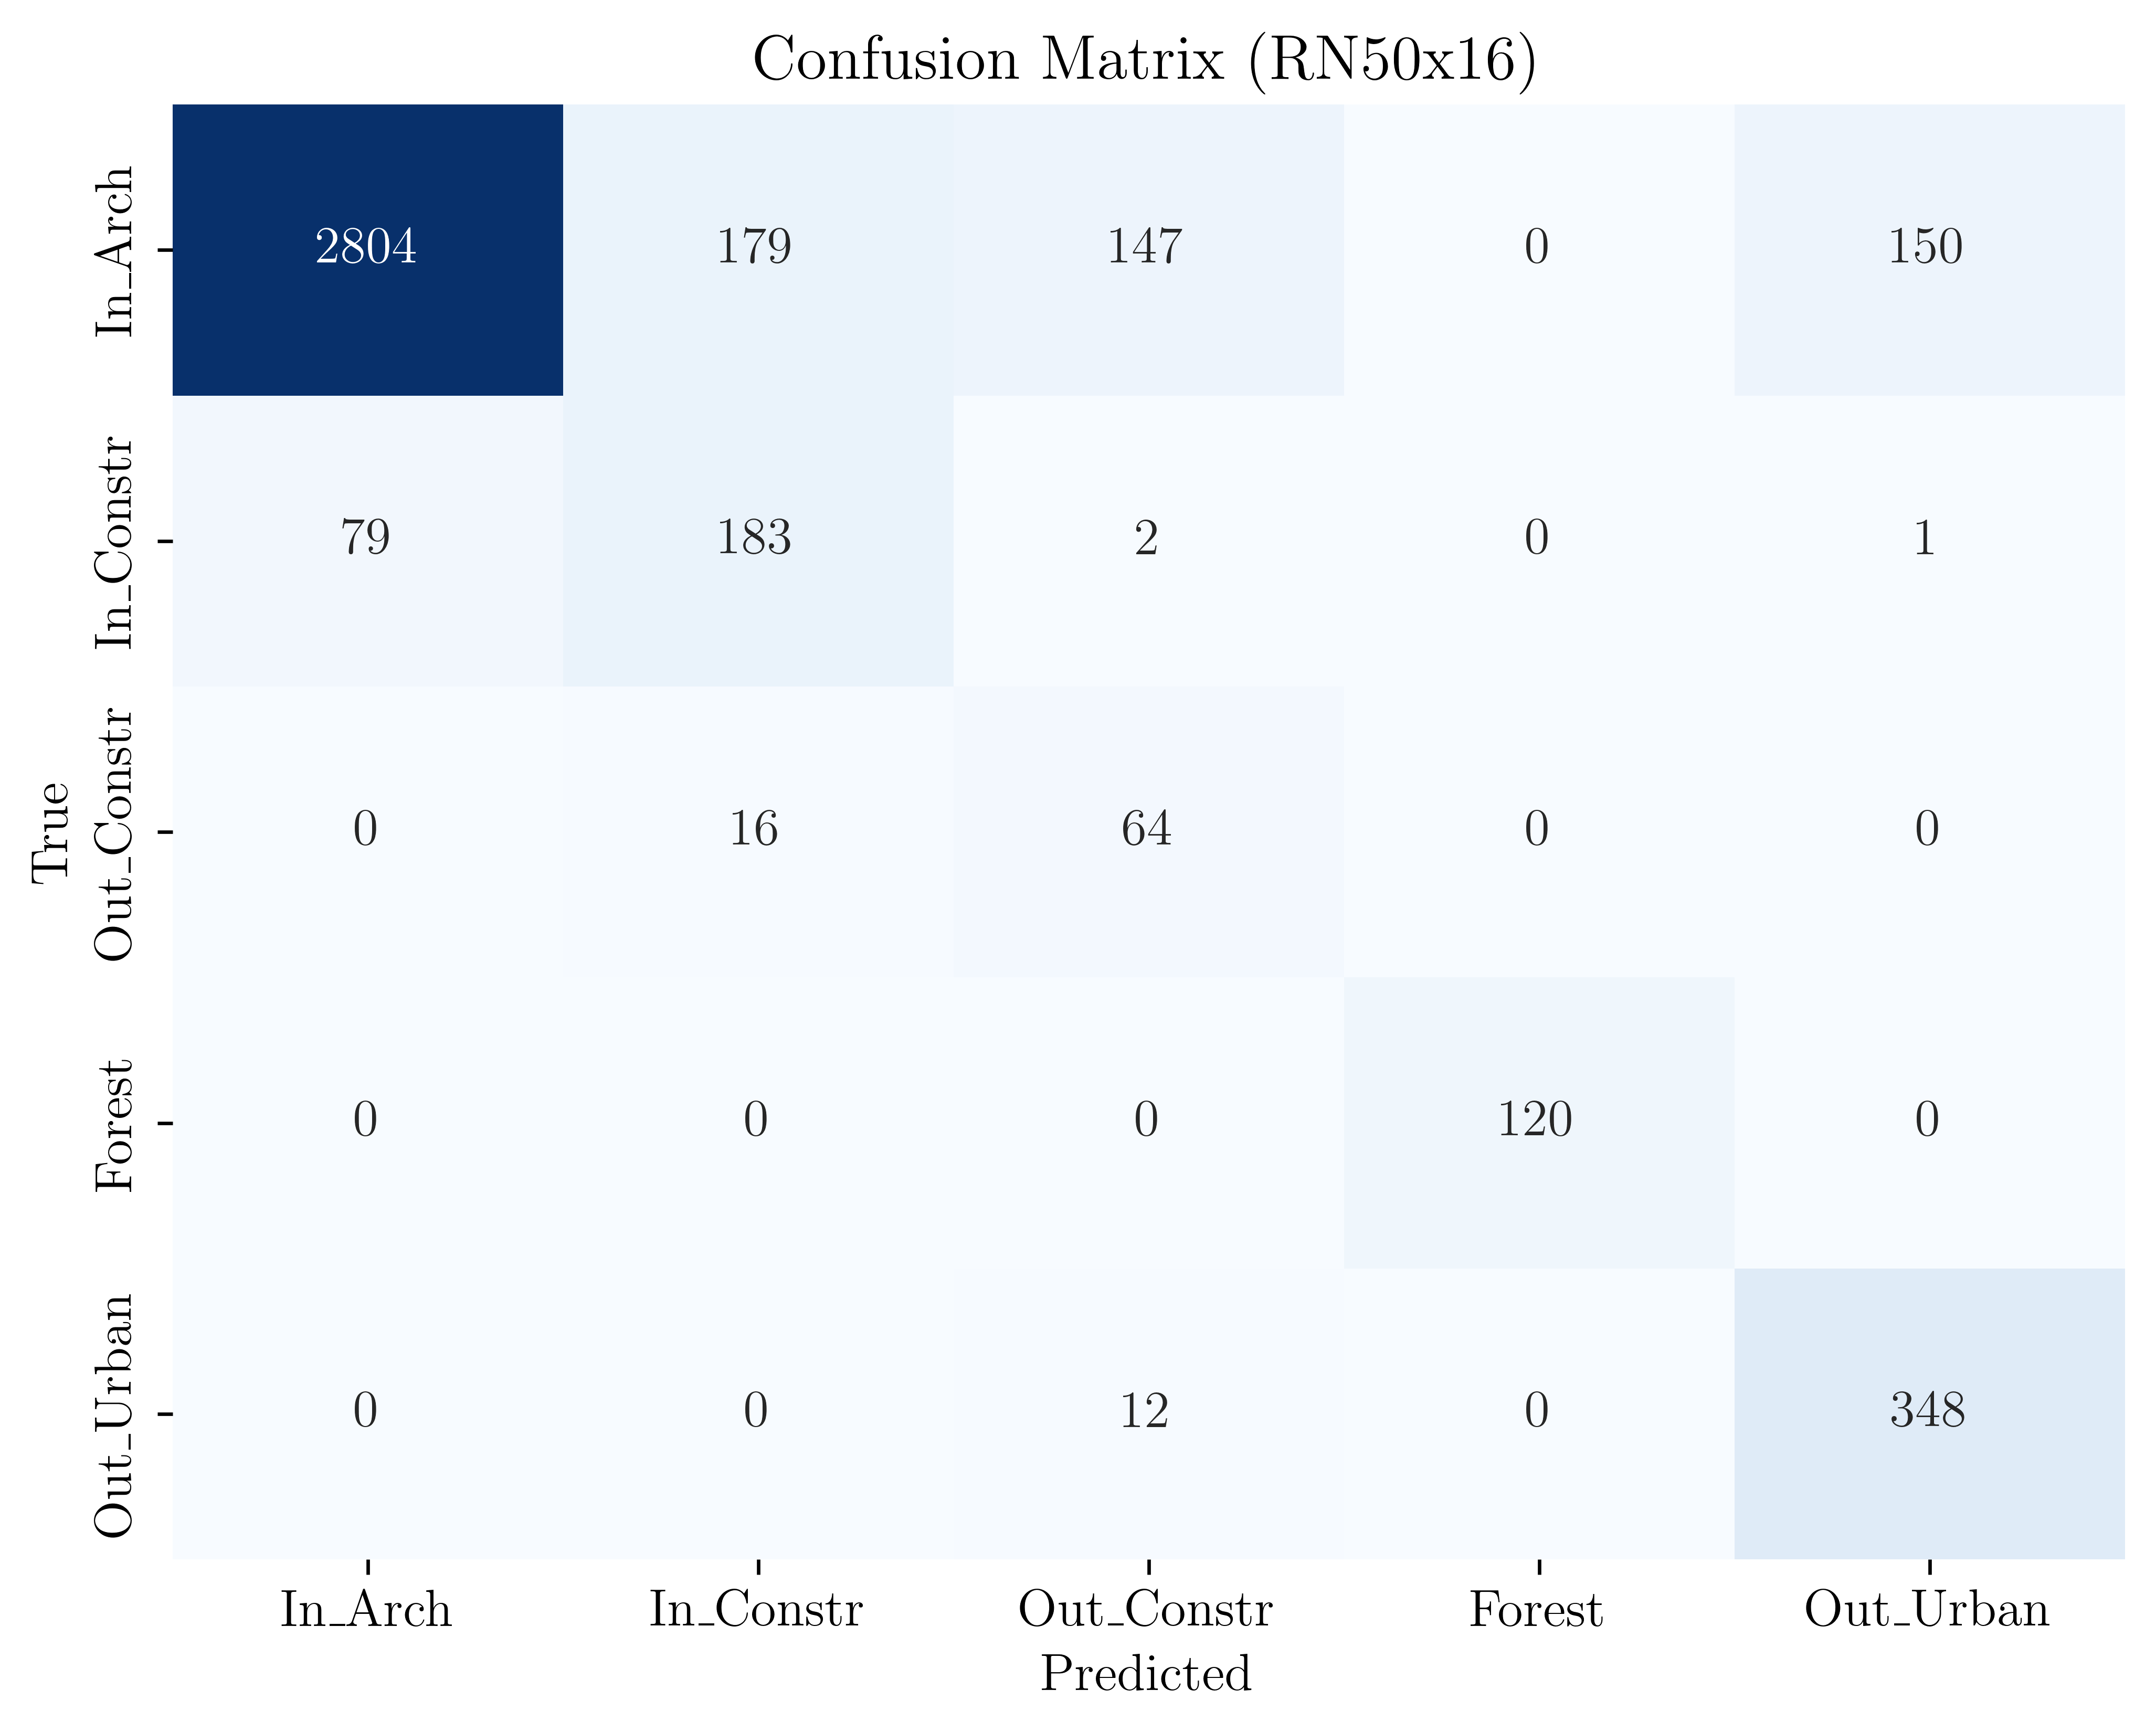
\includegraphics[width=0.49\textwidth]{Images/appendix/resultsPC/Confusion Matrix (RN50x16).png}\label{resultpc:fig:rn50x16}}
    \subfloat[][RN50x64]{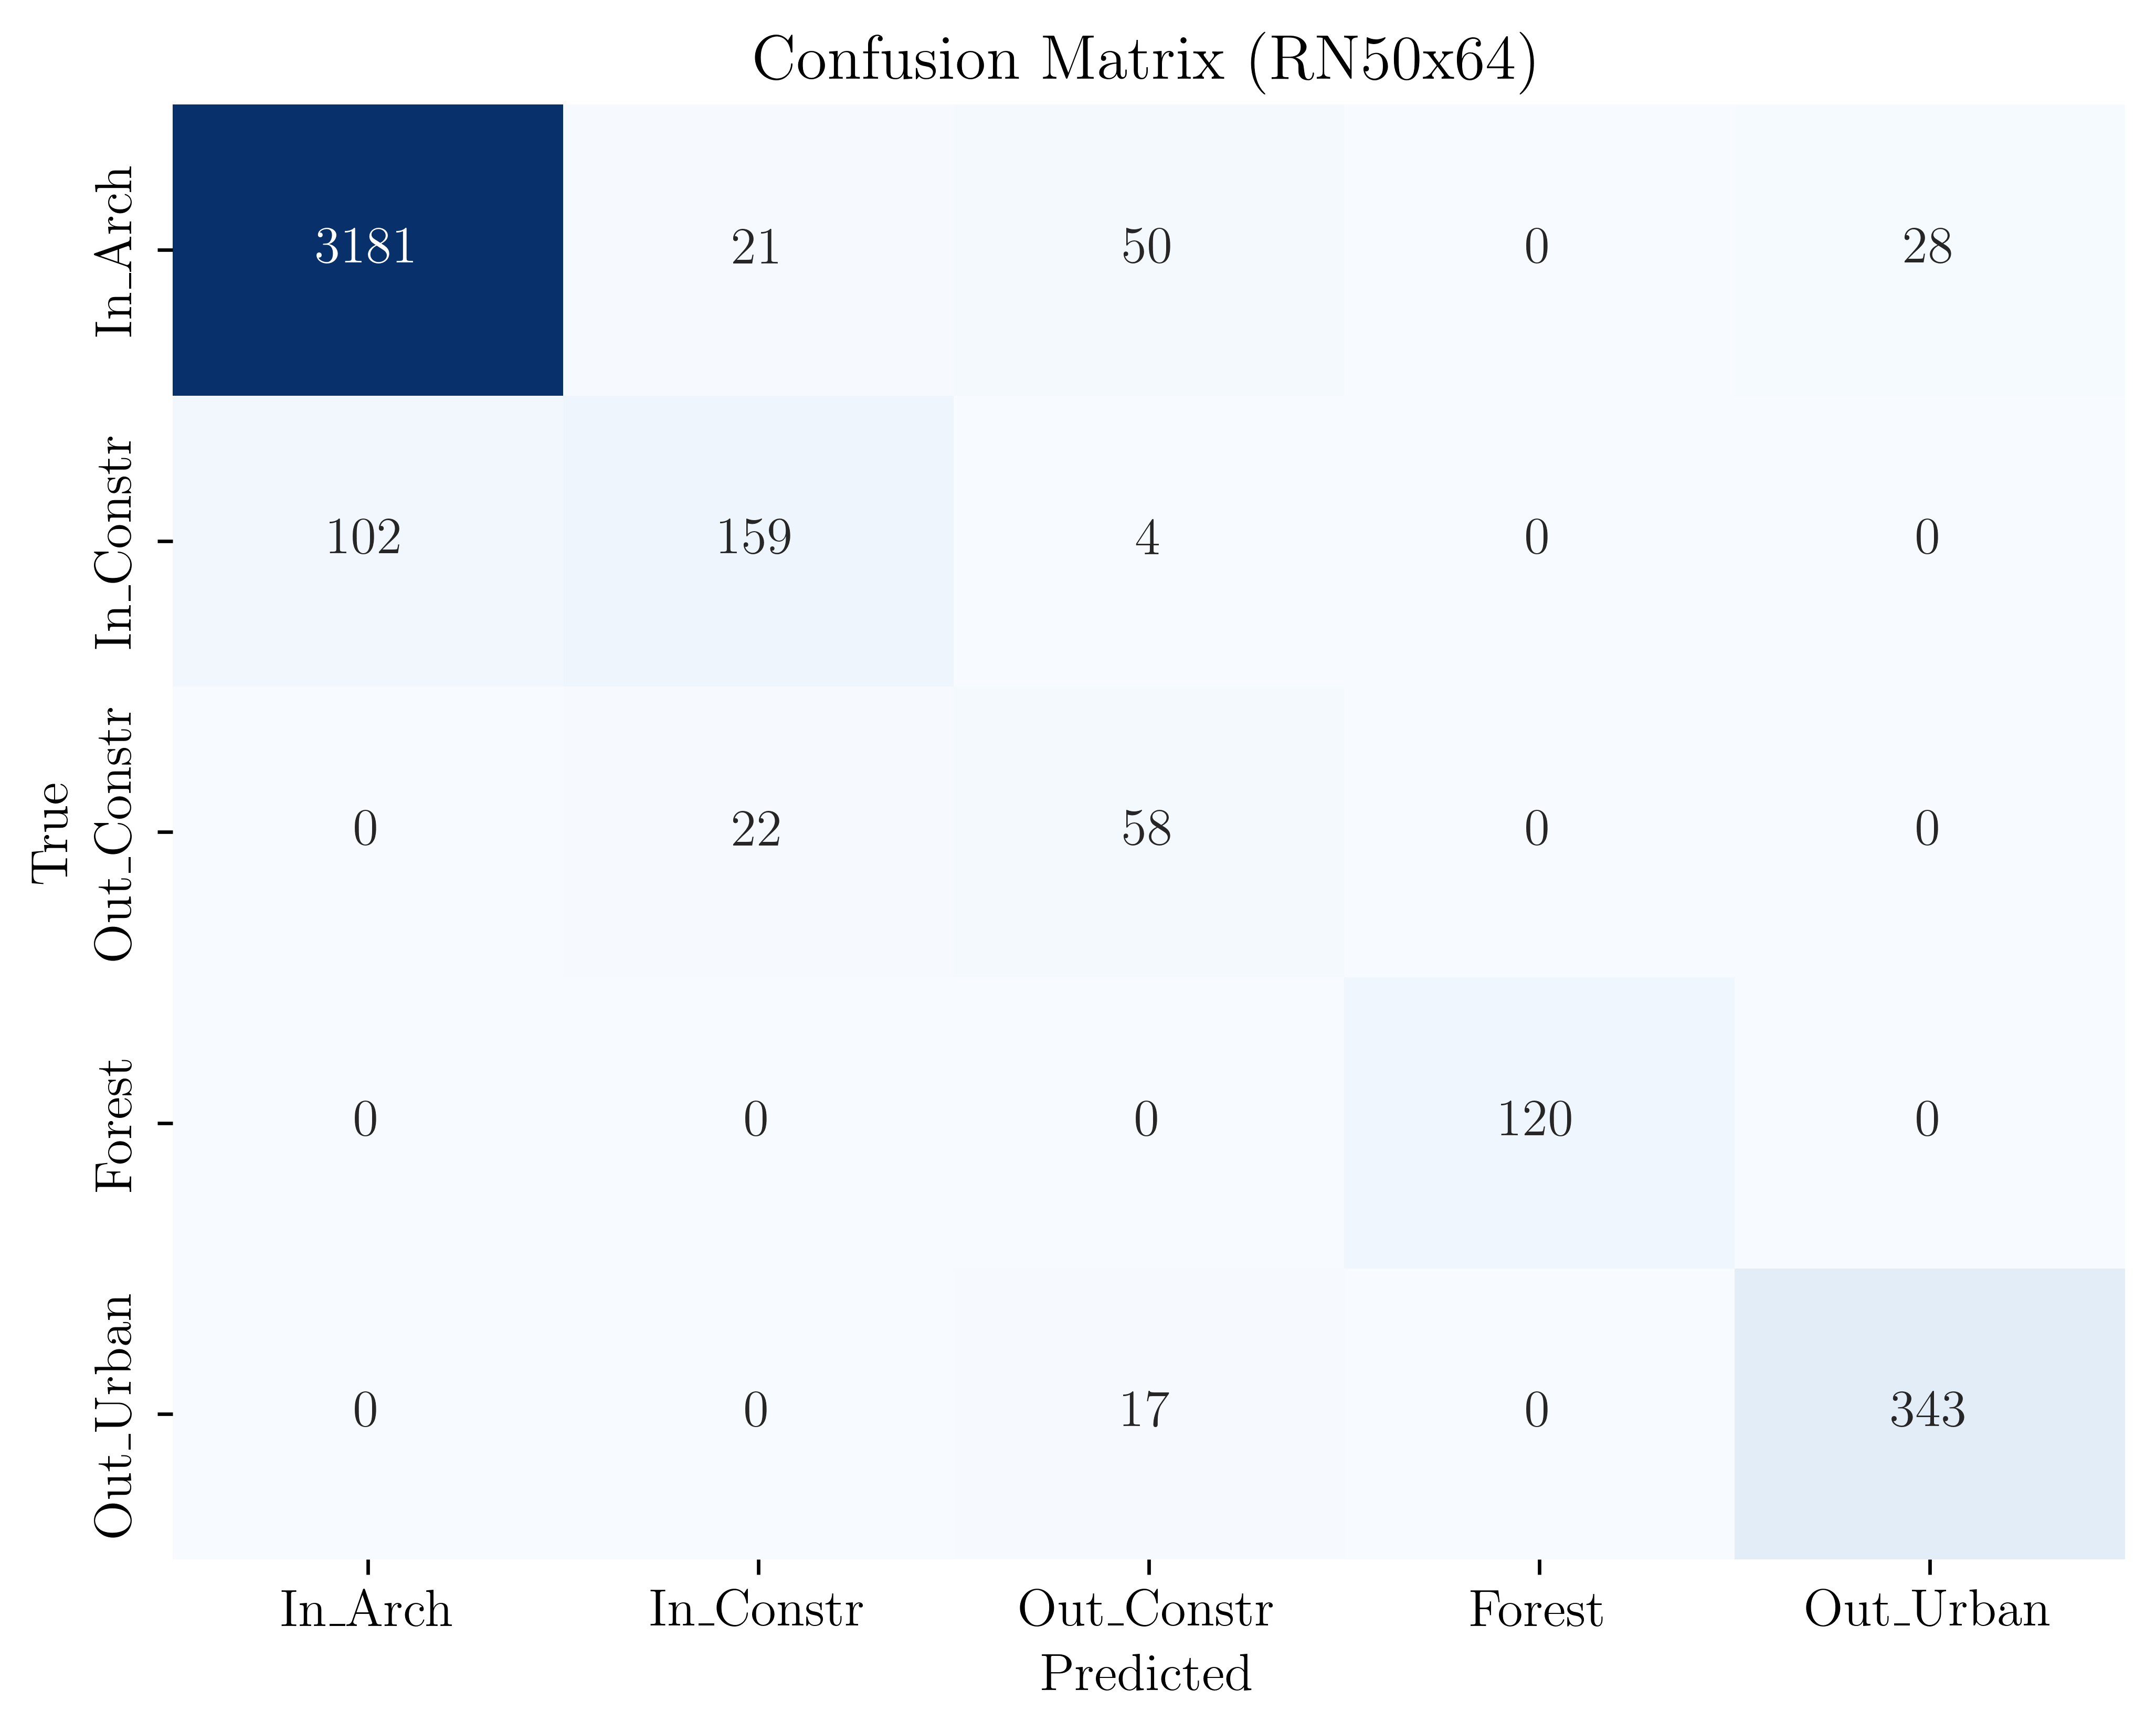
\includegraphics[width=0.49\textwidth]{Images/appendix/resultsPC/Confusion Matrix (RN50x64).png}\label{resultpc:fig:rn50x64}}
\end{figure}

\begin{figure}
    \centering
    %\ContinuedFloat
    \subfloat[][RN101]{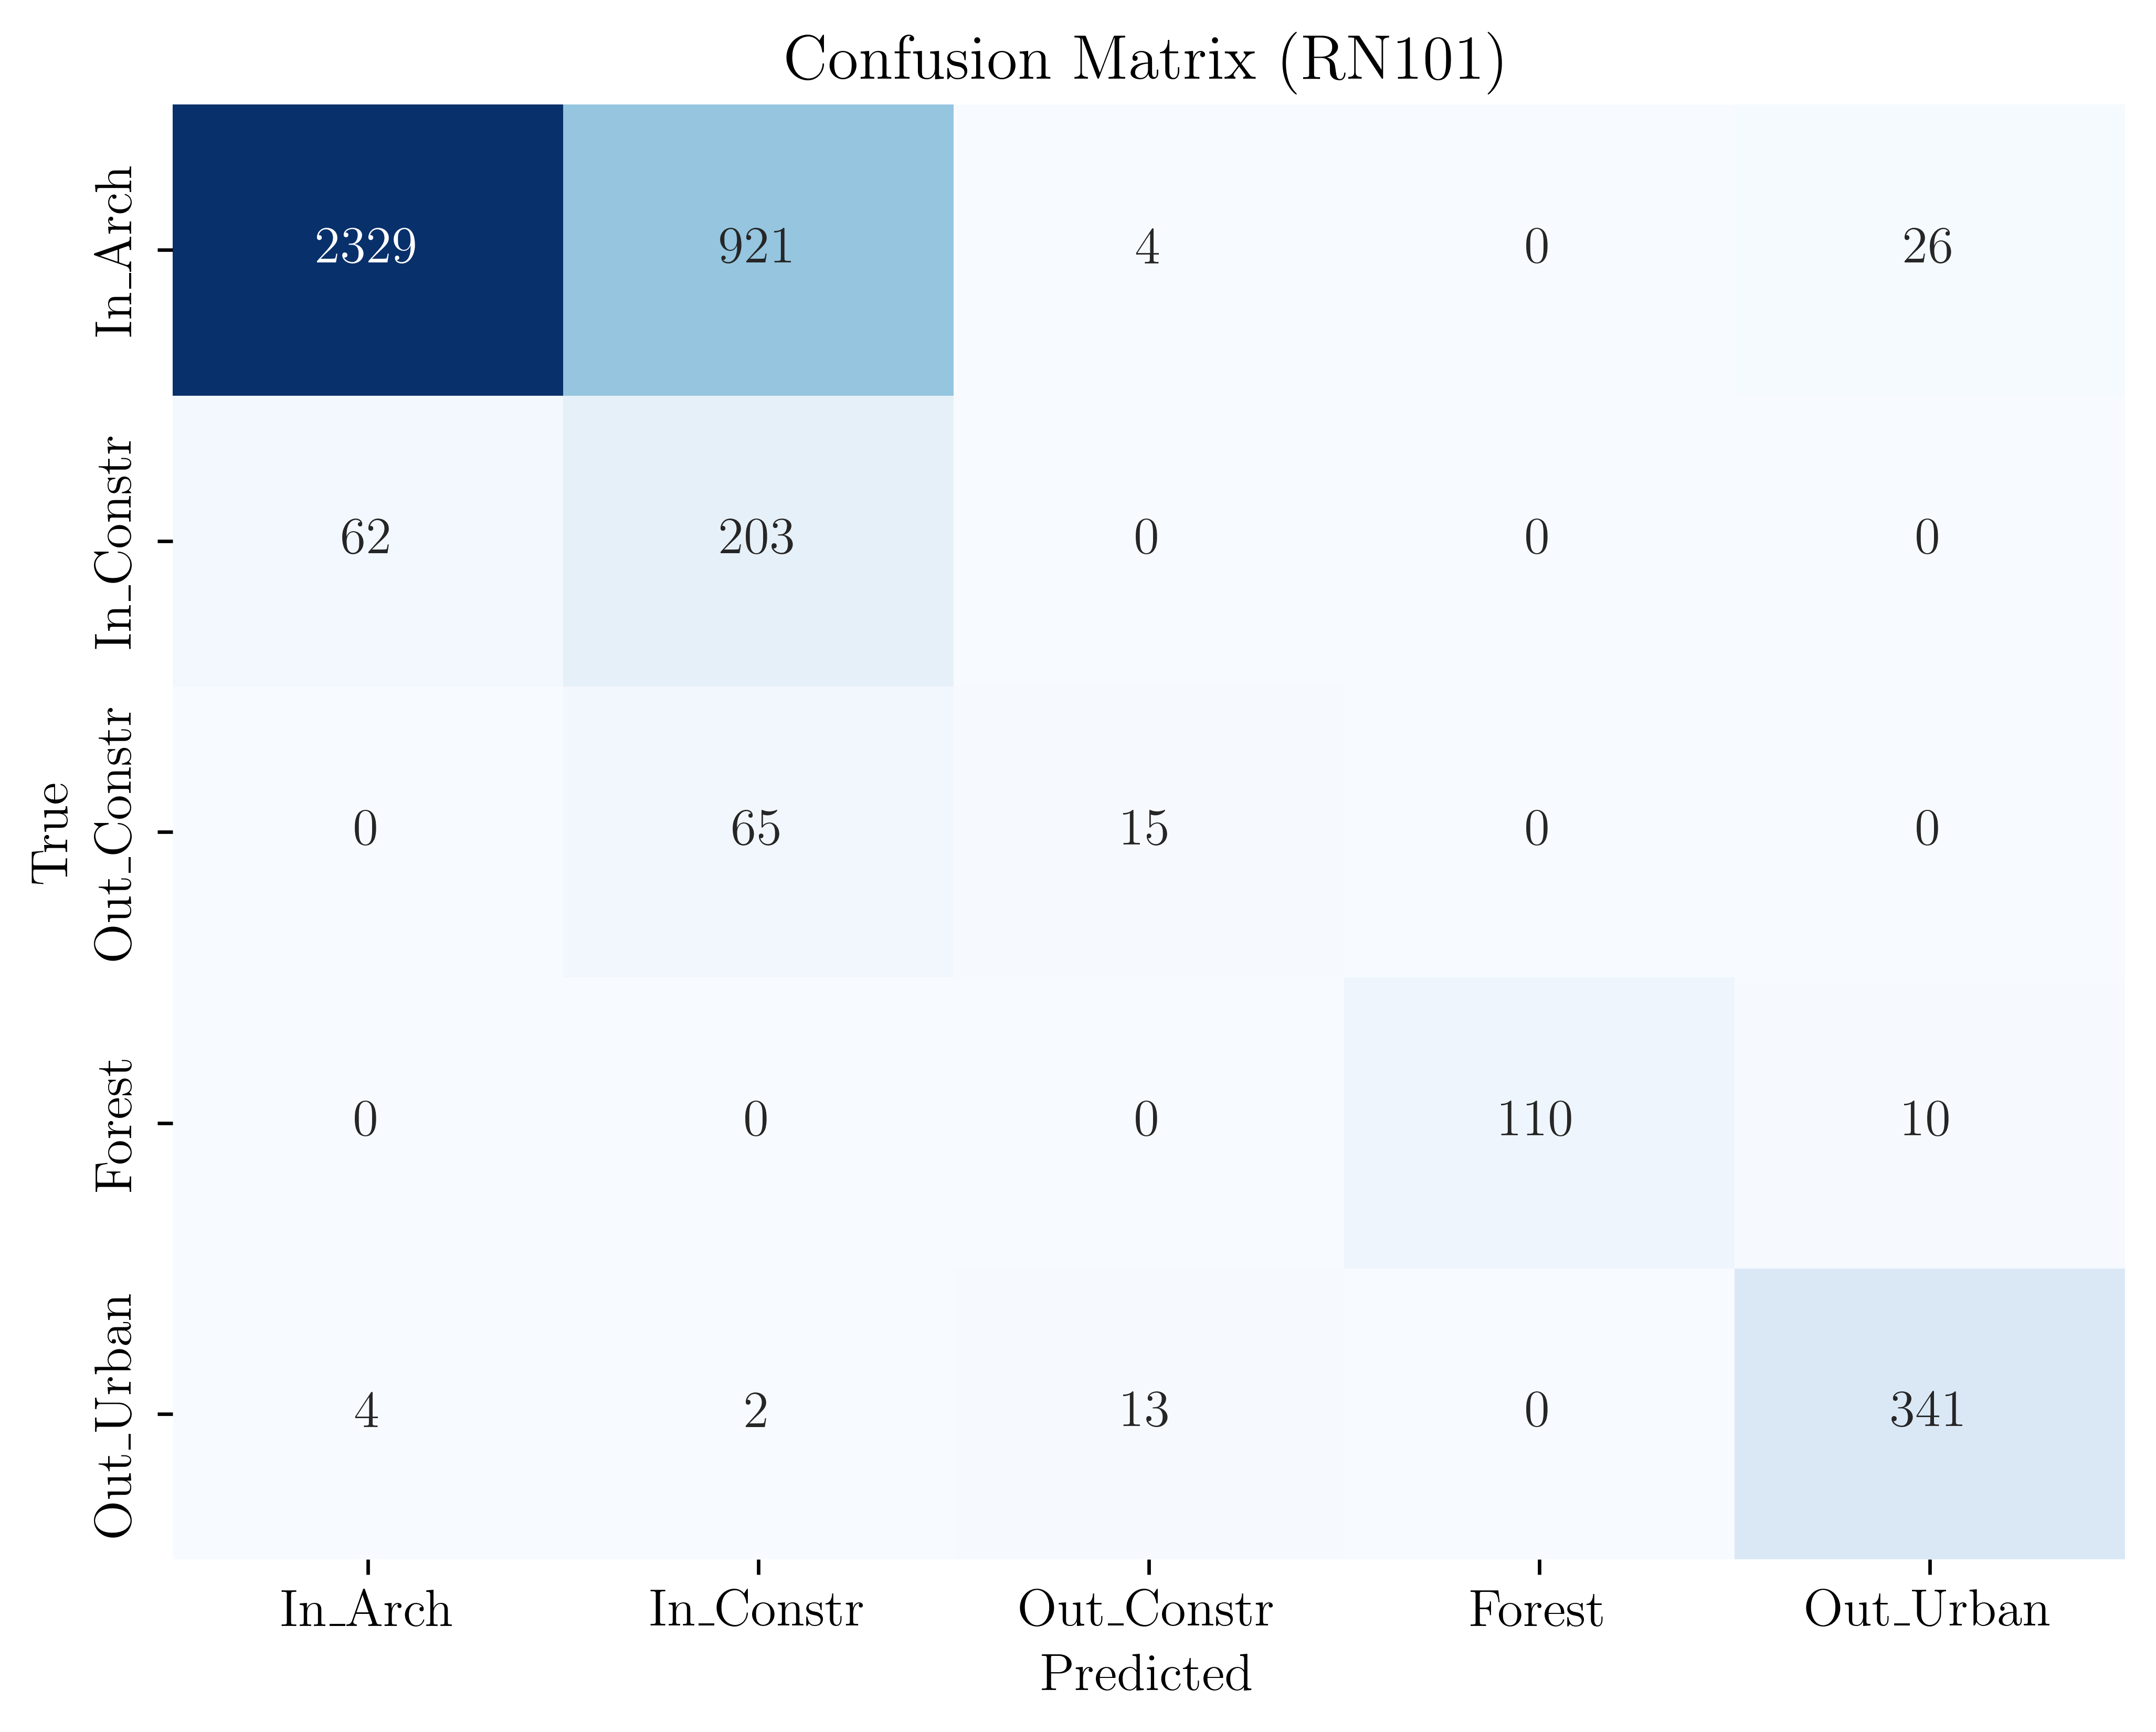
\includegraphics[width=0.49\textwidth]{Images/appendix/resultsPC/Confusion Matrix (RN101).png}\label{resultpc:fig:rn101}}
    \subfloat[][TinyCLIP 19M]{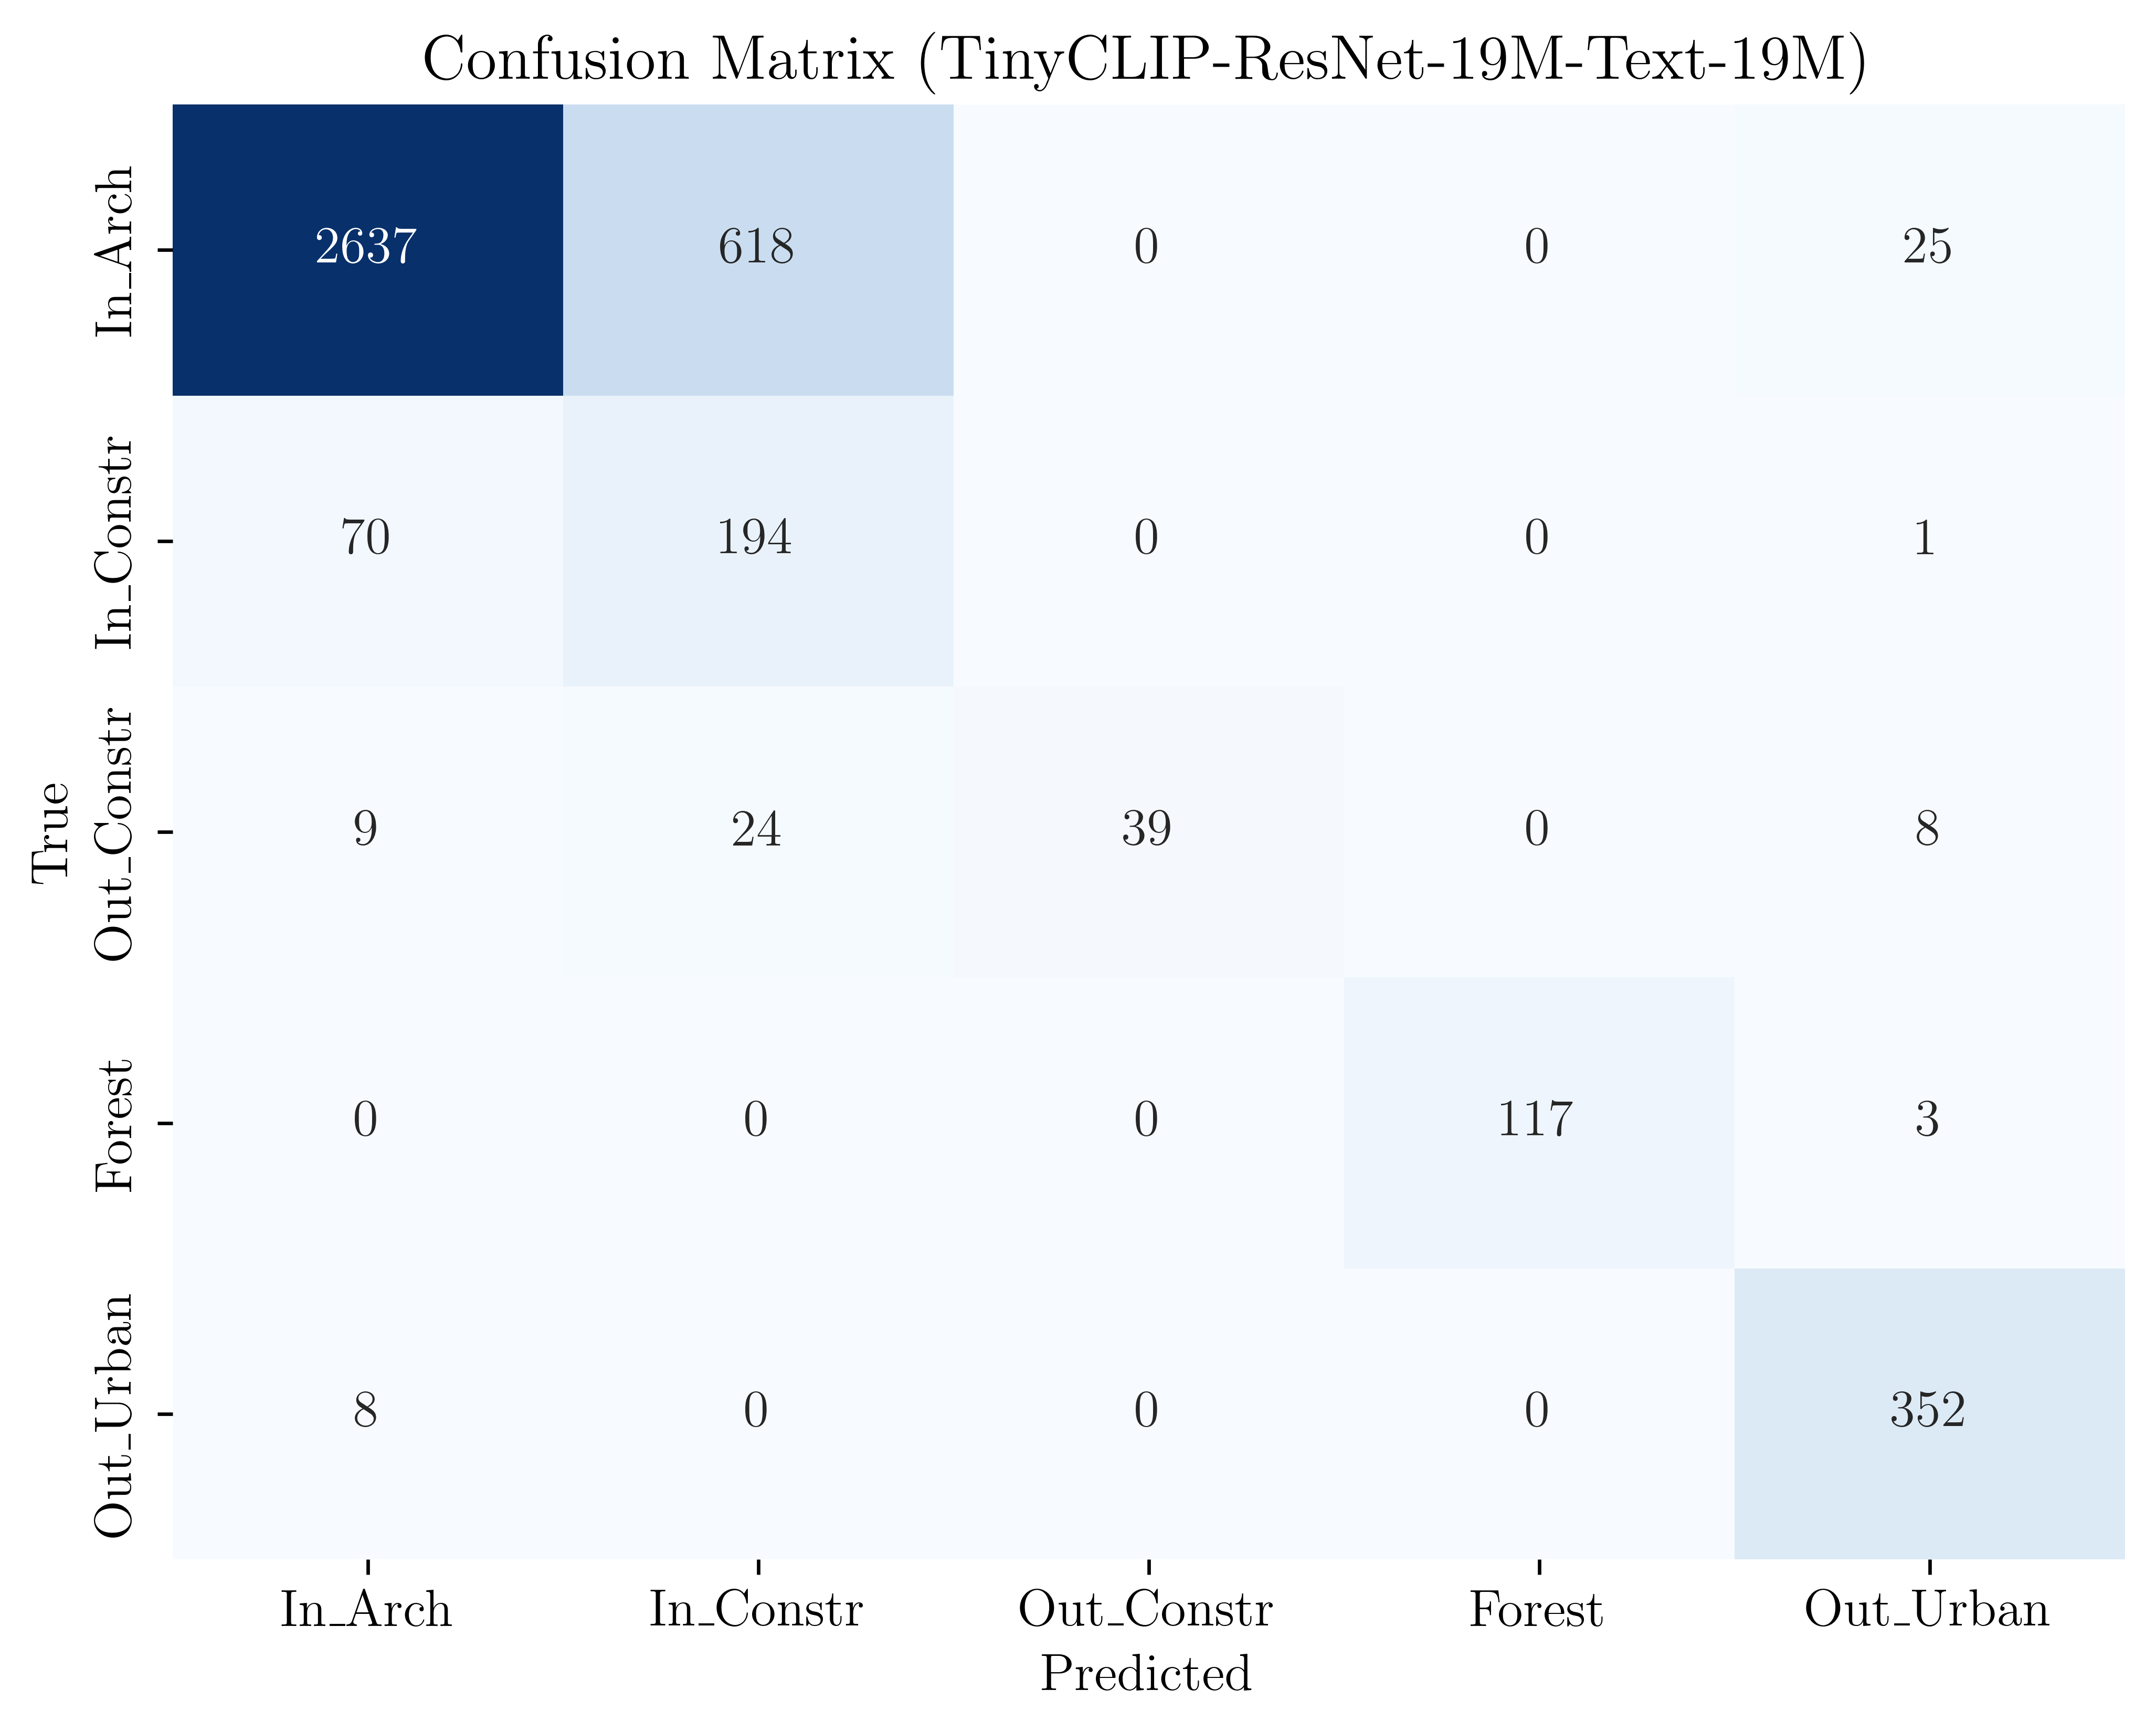
\includegraphics[width=0.49\textwidth]{Images/appendix/resultsPC/Confusion Matrix (TinyCLIP-ResNet-19M-Text-19M).png}\label{resultpc:fig:tiny19}}
    \quad
    \subfloat[][TinyCLIP 30M]{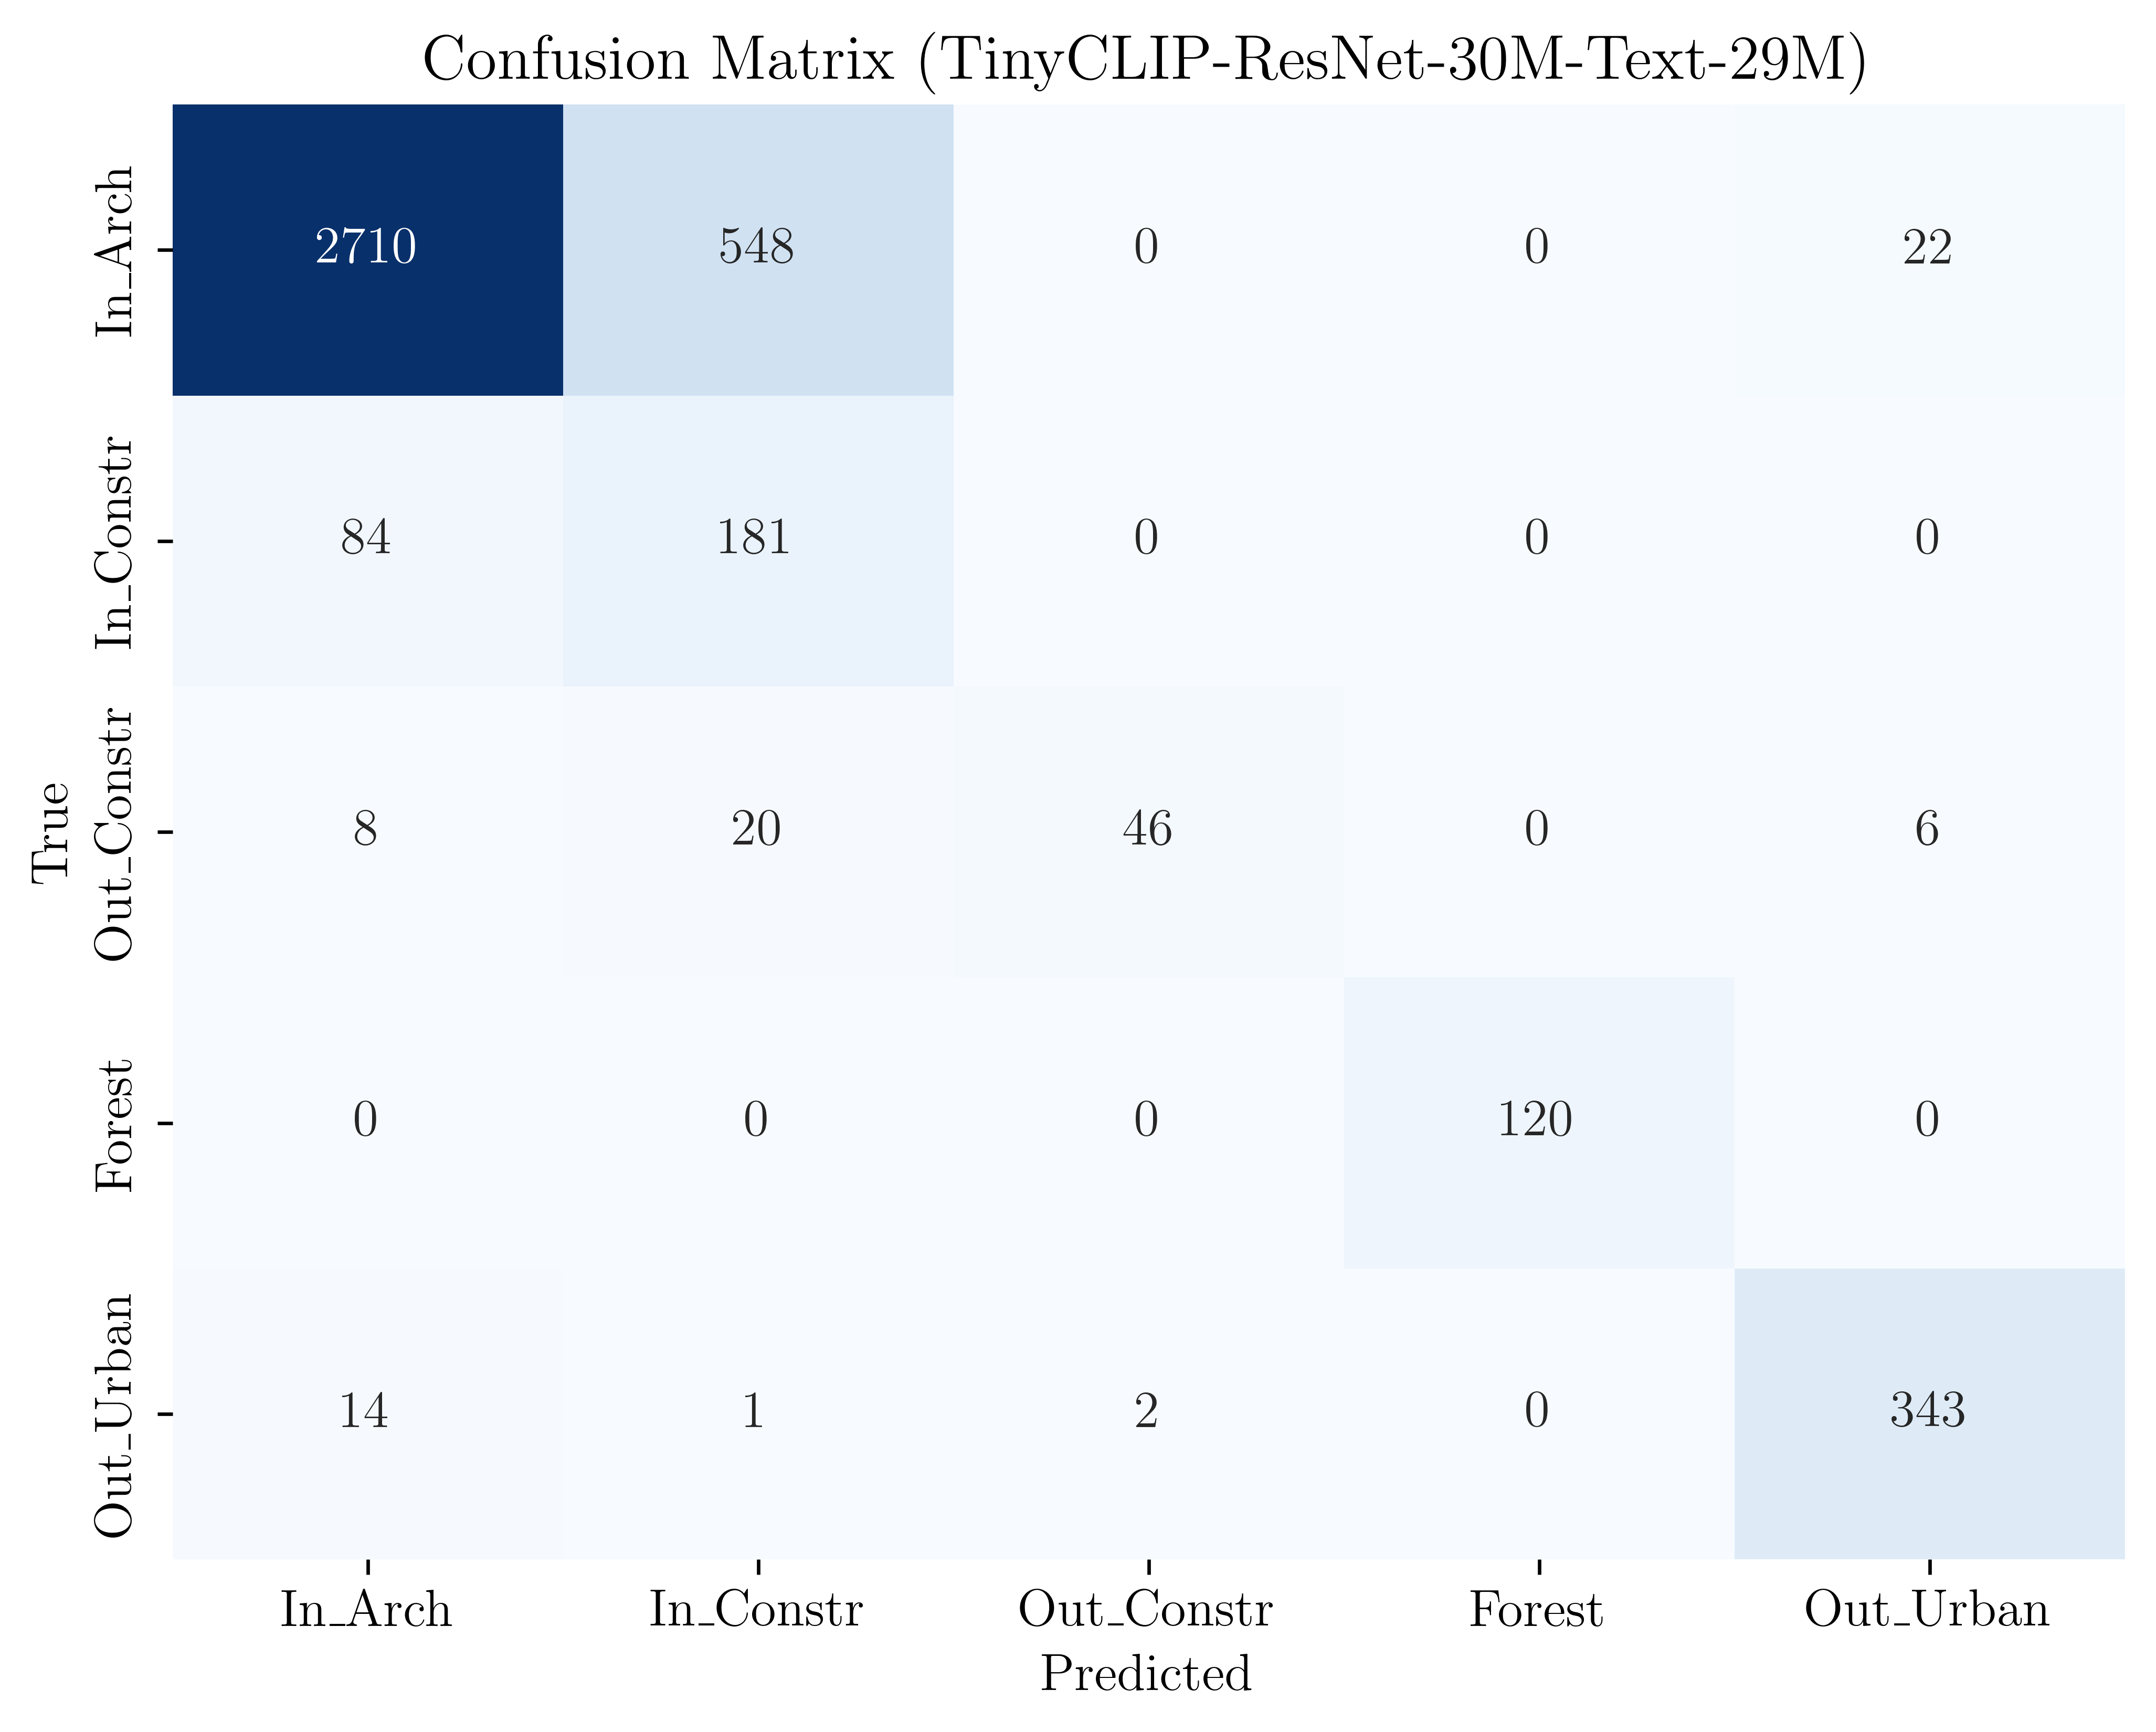
\includegraphics[width=0.49\textwidth]{Images/appendix/resultsPC/Confusion Matrix (TinyCLIP-ResNet-30M-Text-29M).png}\label{resultpc:fig:tiny30}}
    \label{resultpc:fig:evalpc}
    \caption{Confusion matrix on PC with pure text prompts as text embeddings}
\end{figure}
    \chapter{Evaluation on Raspberry Pi CPU}
The following figures are the confusion matrices evaluation on PC CPU.
\begin{figure}[!h]
    \centering
    \subfloat[][TinyClip19M]{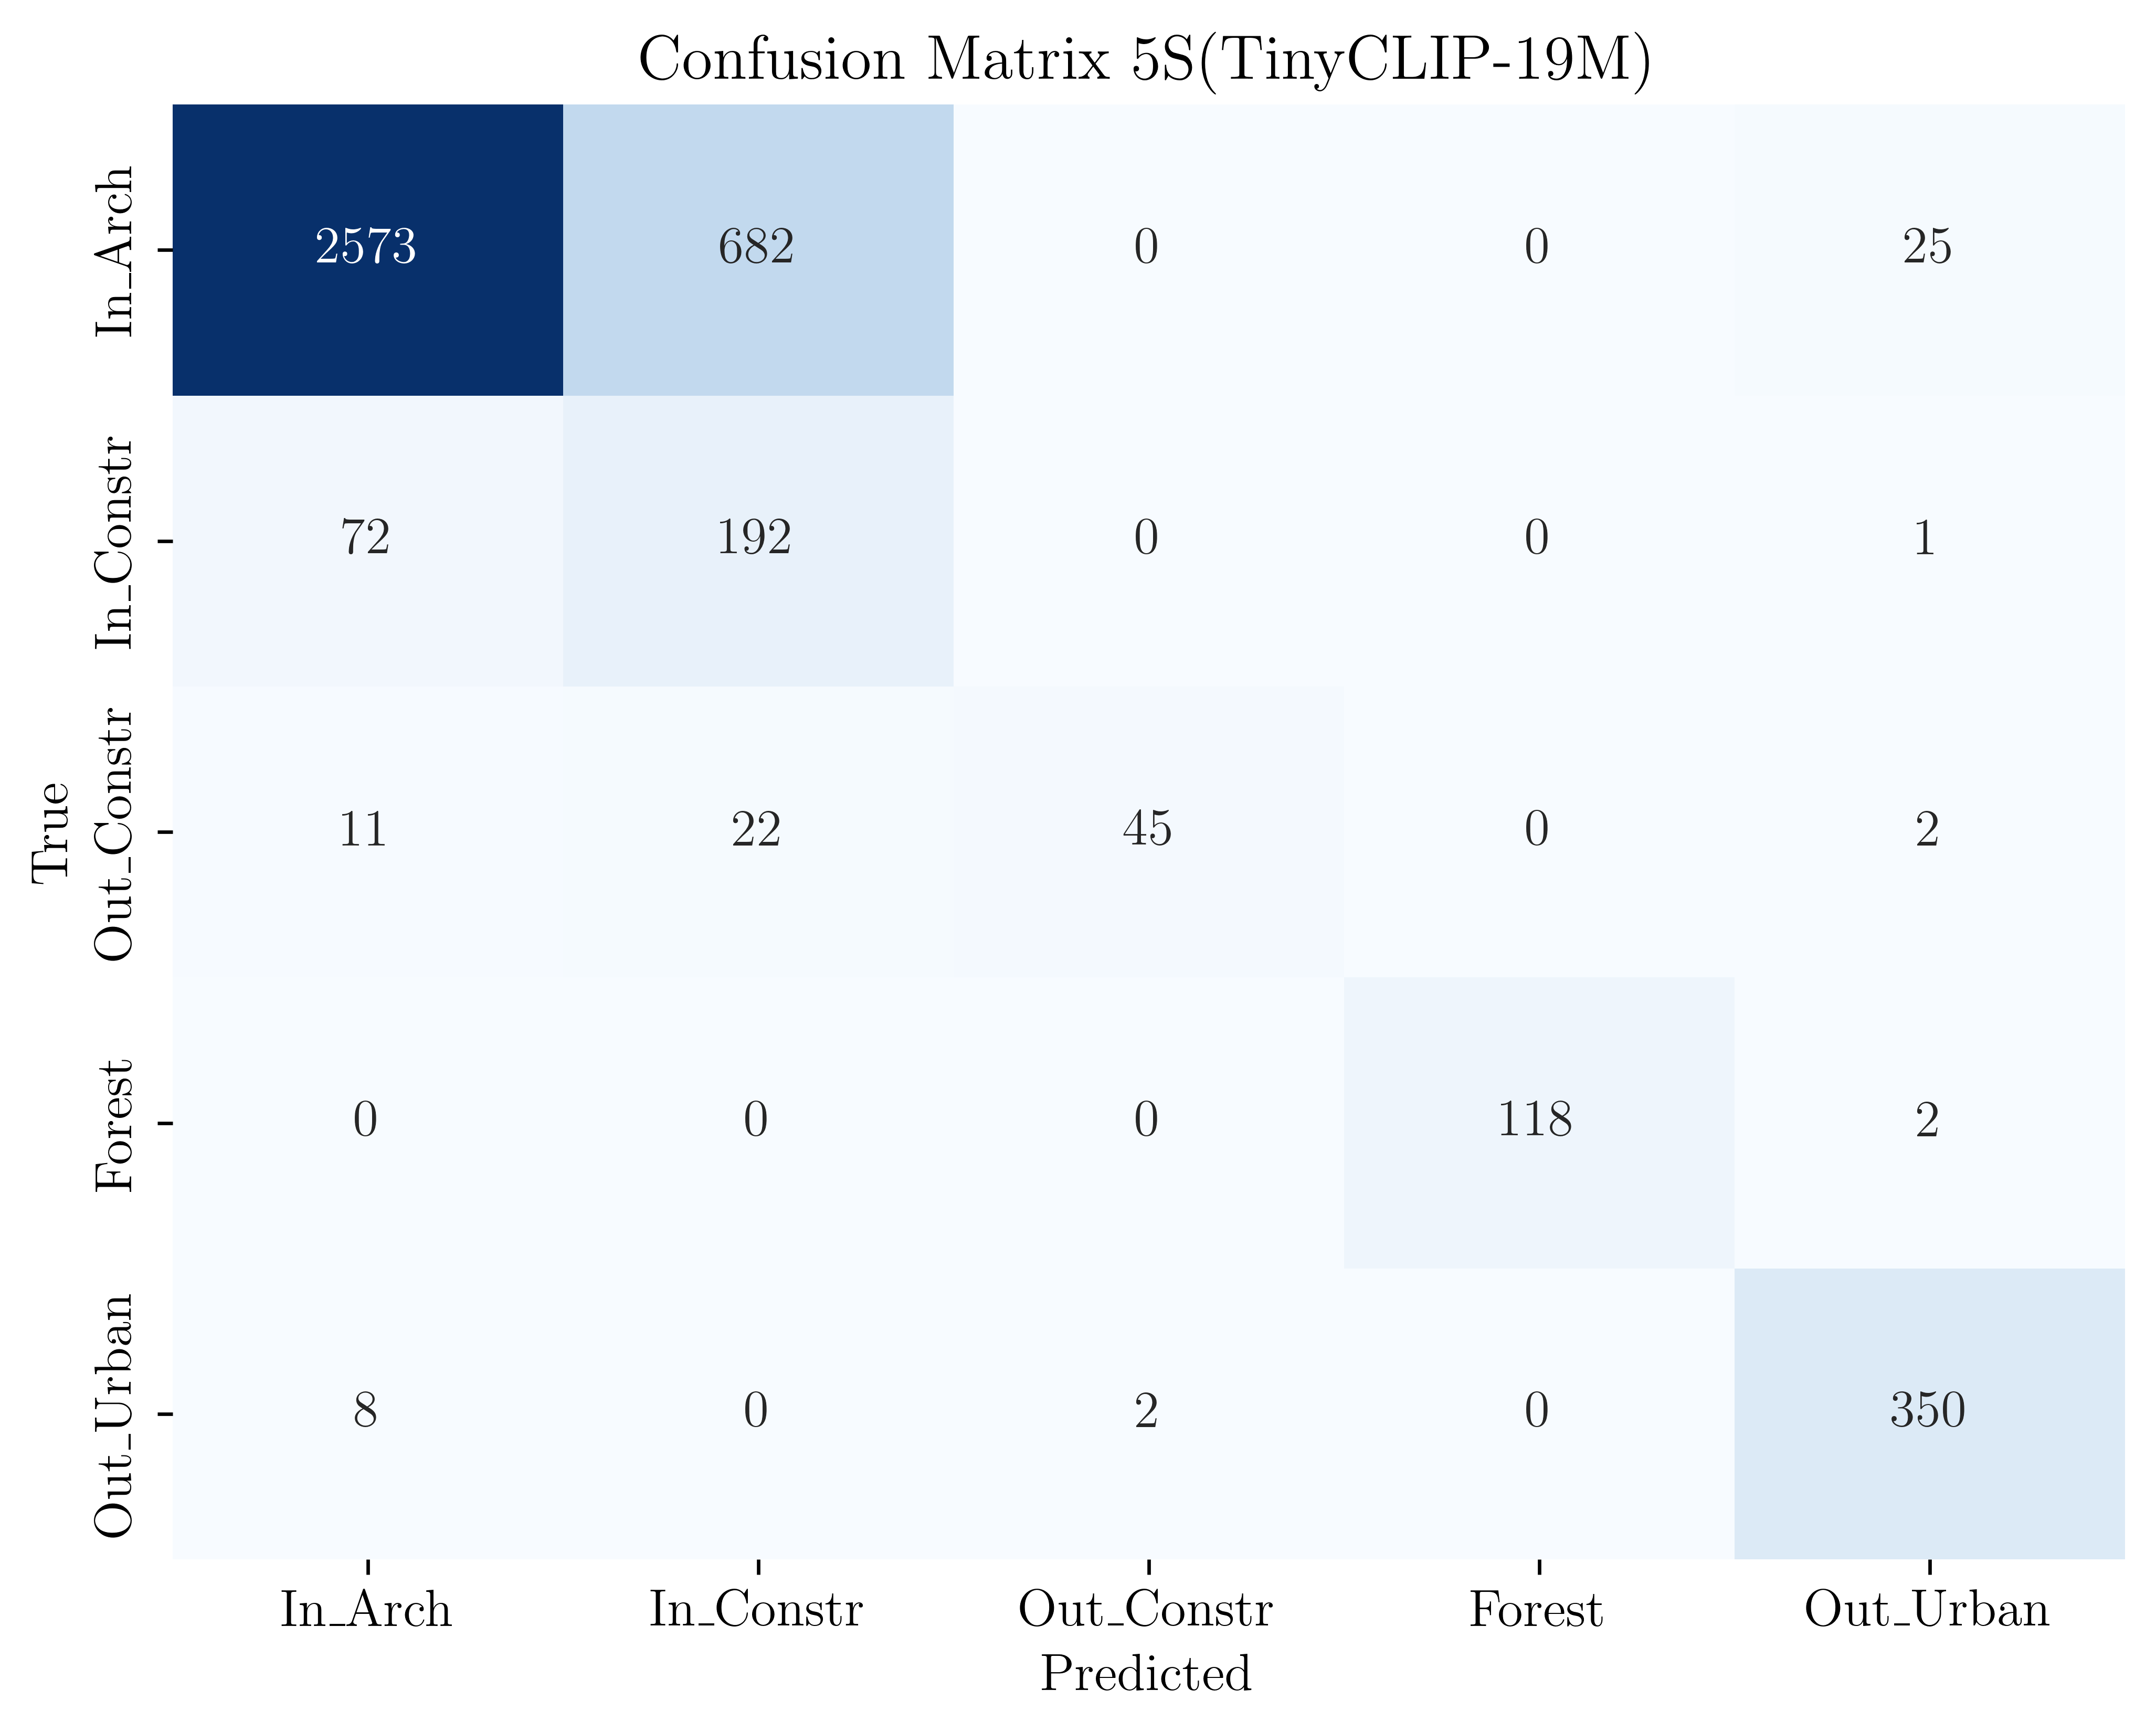
\includegraphics[width=0.45\textwidth]{Images/appendix/resultsRaspi/Confusion Matrix 5S(TinyCLIP-19M).png}\label{resultpc:fig:tiny19M5s}}
    \subfloat[][TinyClip30M]{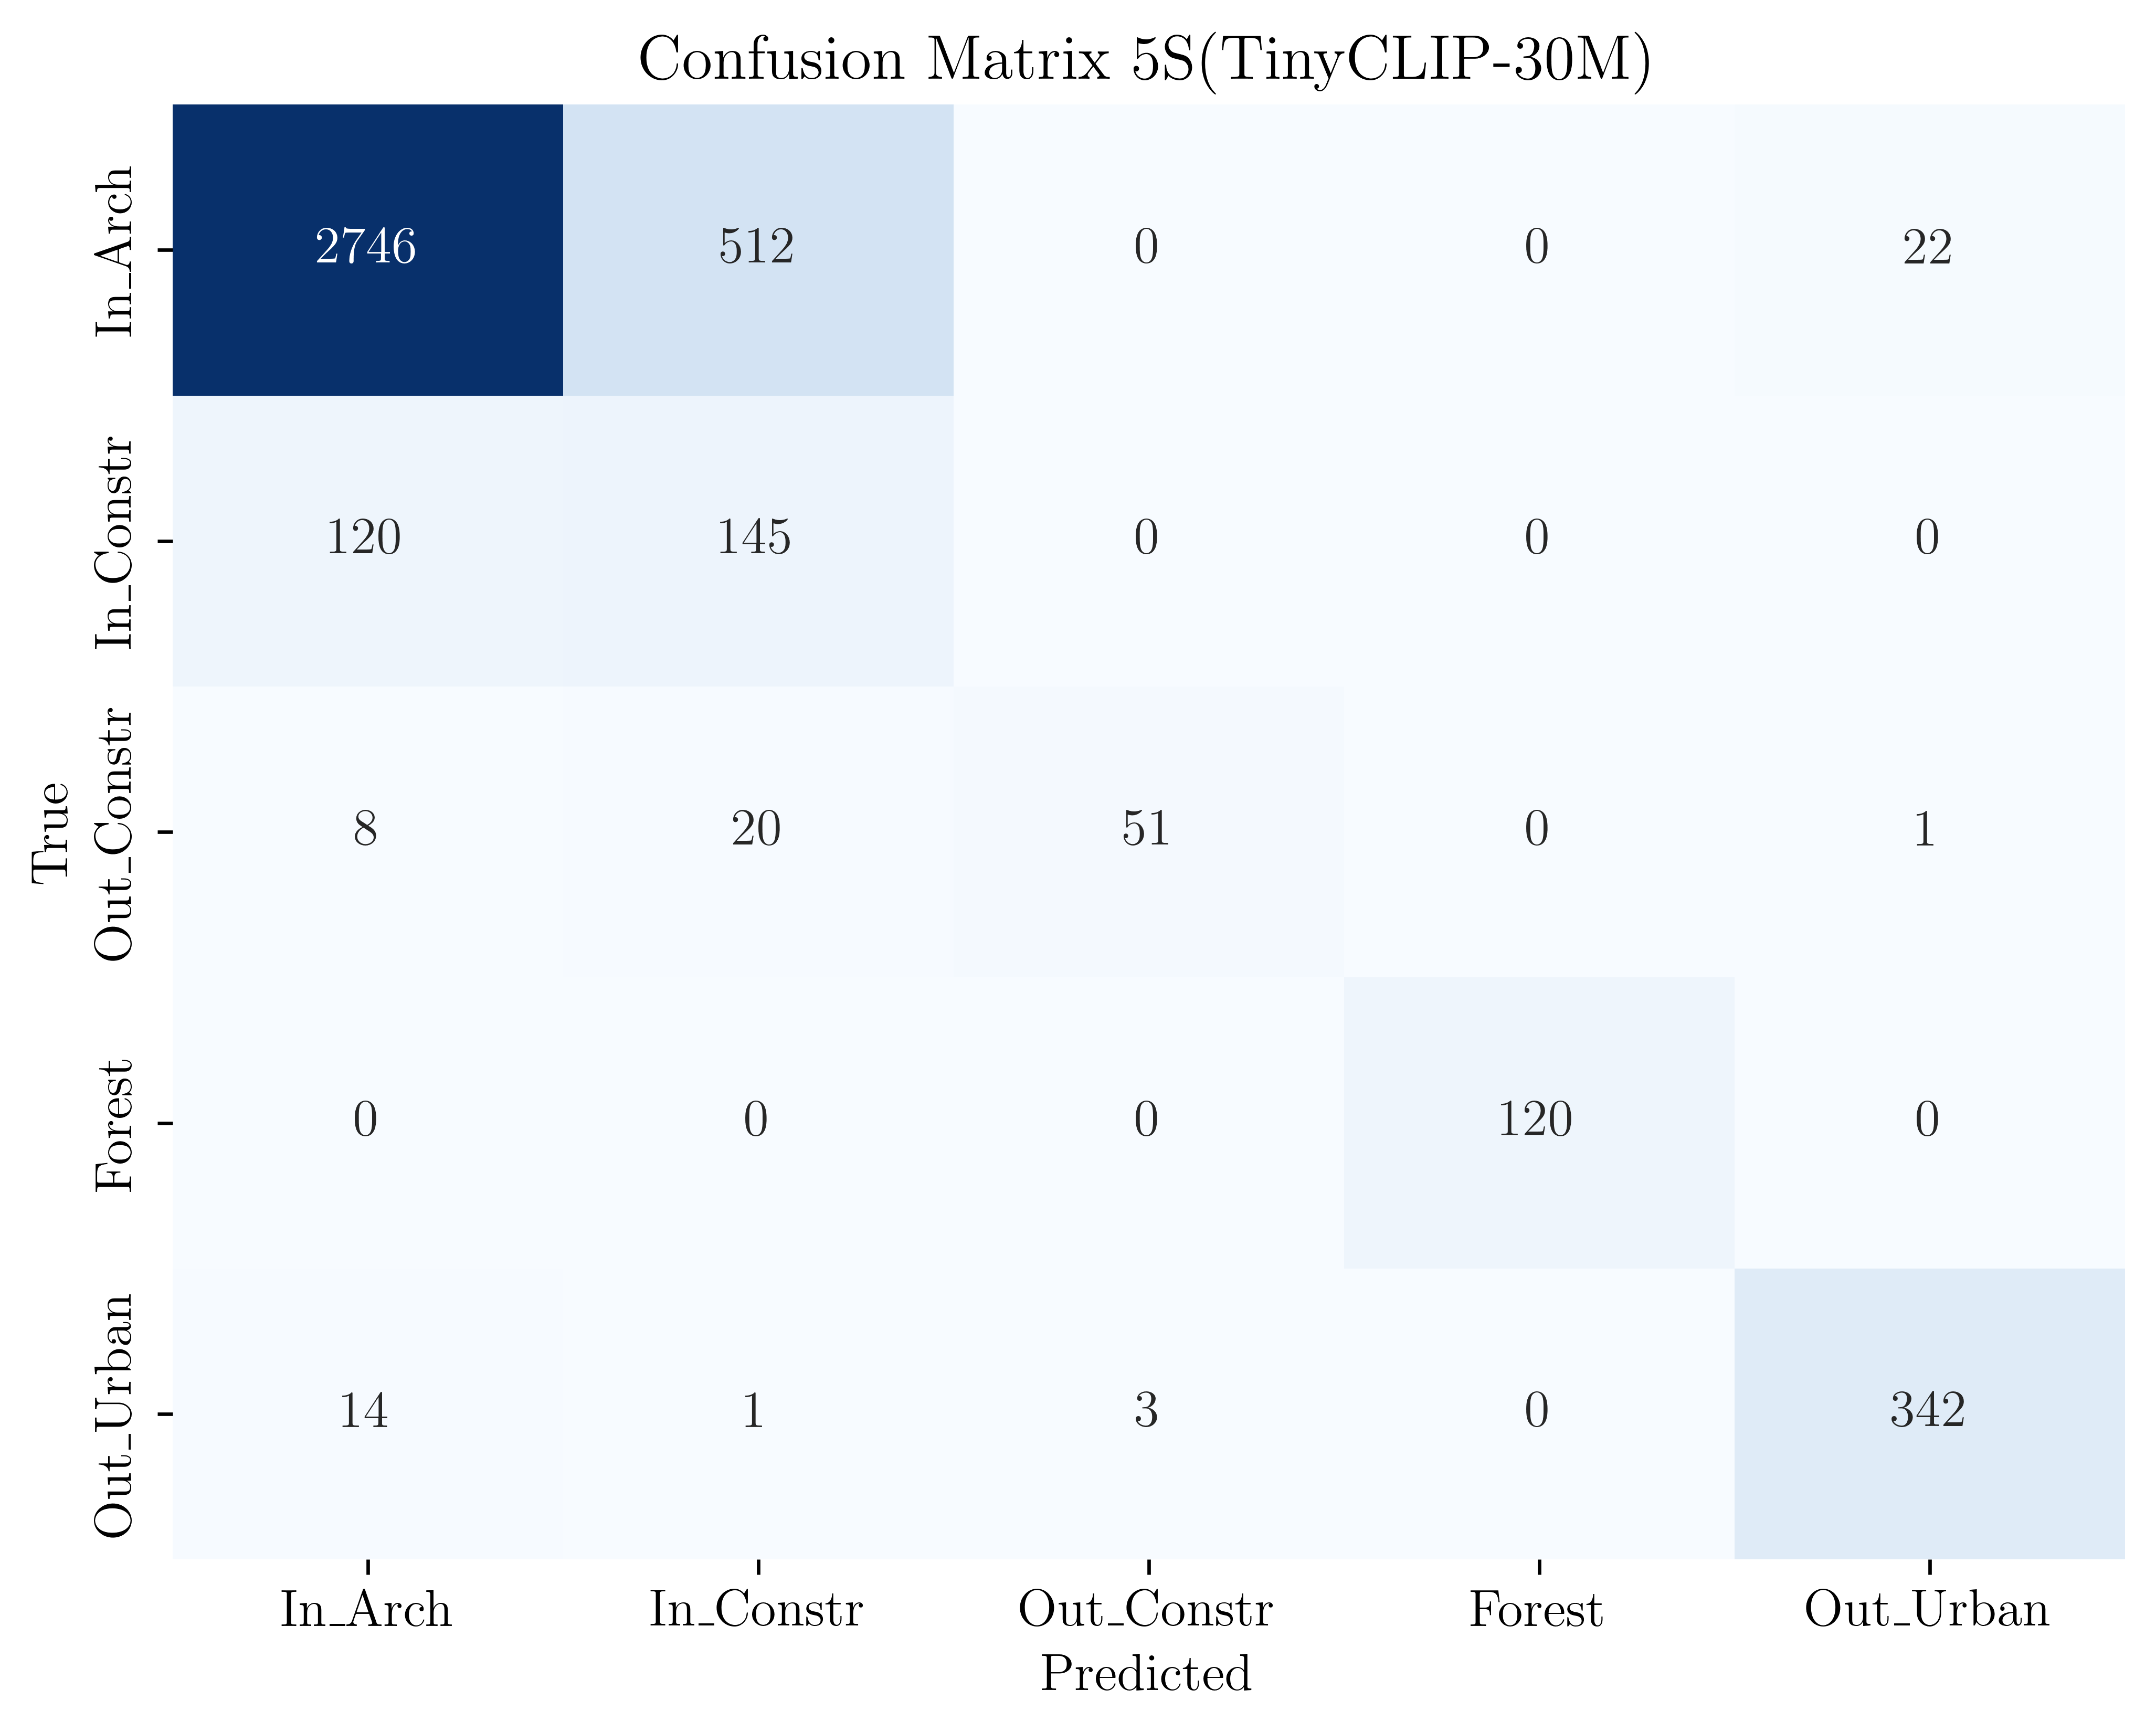
\includegraphics[width=0.45\textwidth]{Images/appendix/resultsRaspi/Confusion Matrix 5S(TinyCLIP-30M).png}\label{resultpc:fig:tiny30M5s}}
    \caption{Confusion Matrix on Raspberry Pi CPU for TinyCLIP with ResNets as Visual Encoder (5 Sentences as Text Embeddings)}
    \label{resultpc:fig:tinyclipevalraspi5s}
\end{figure}
\begin{figure}[!h]
    \centering
    \subfloat[][RN50]{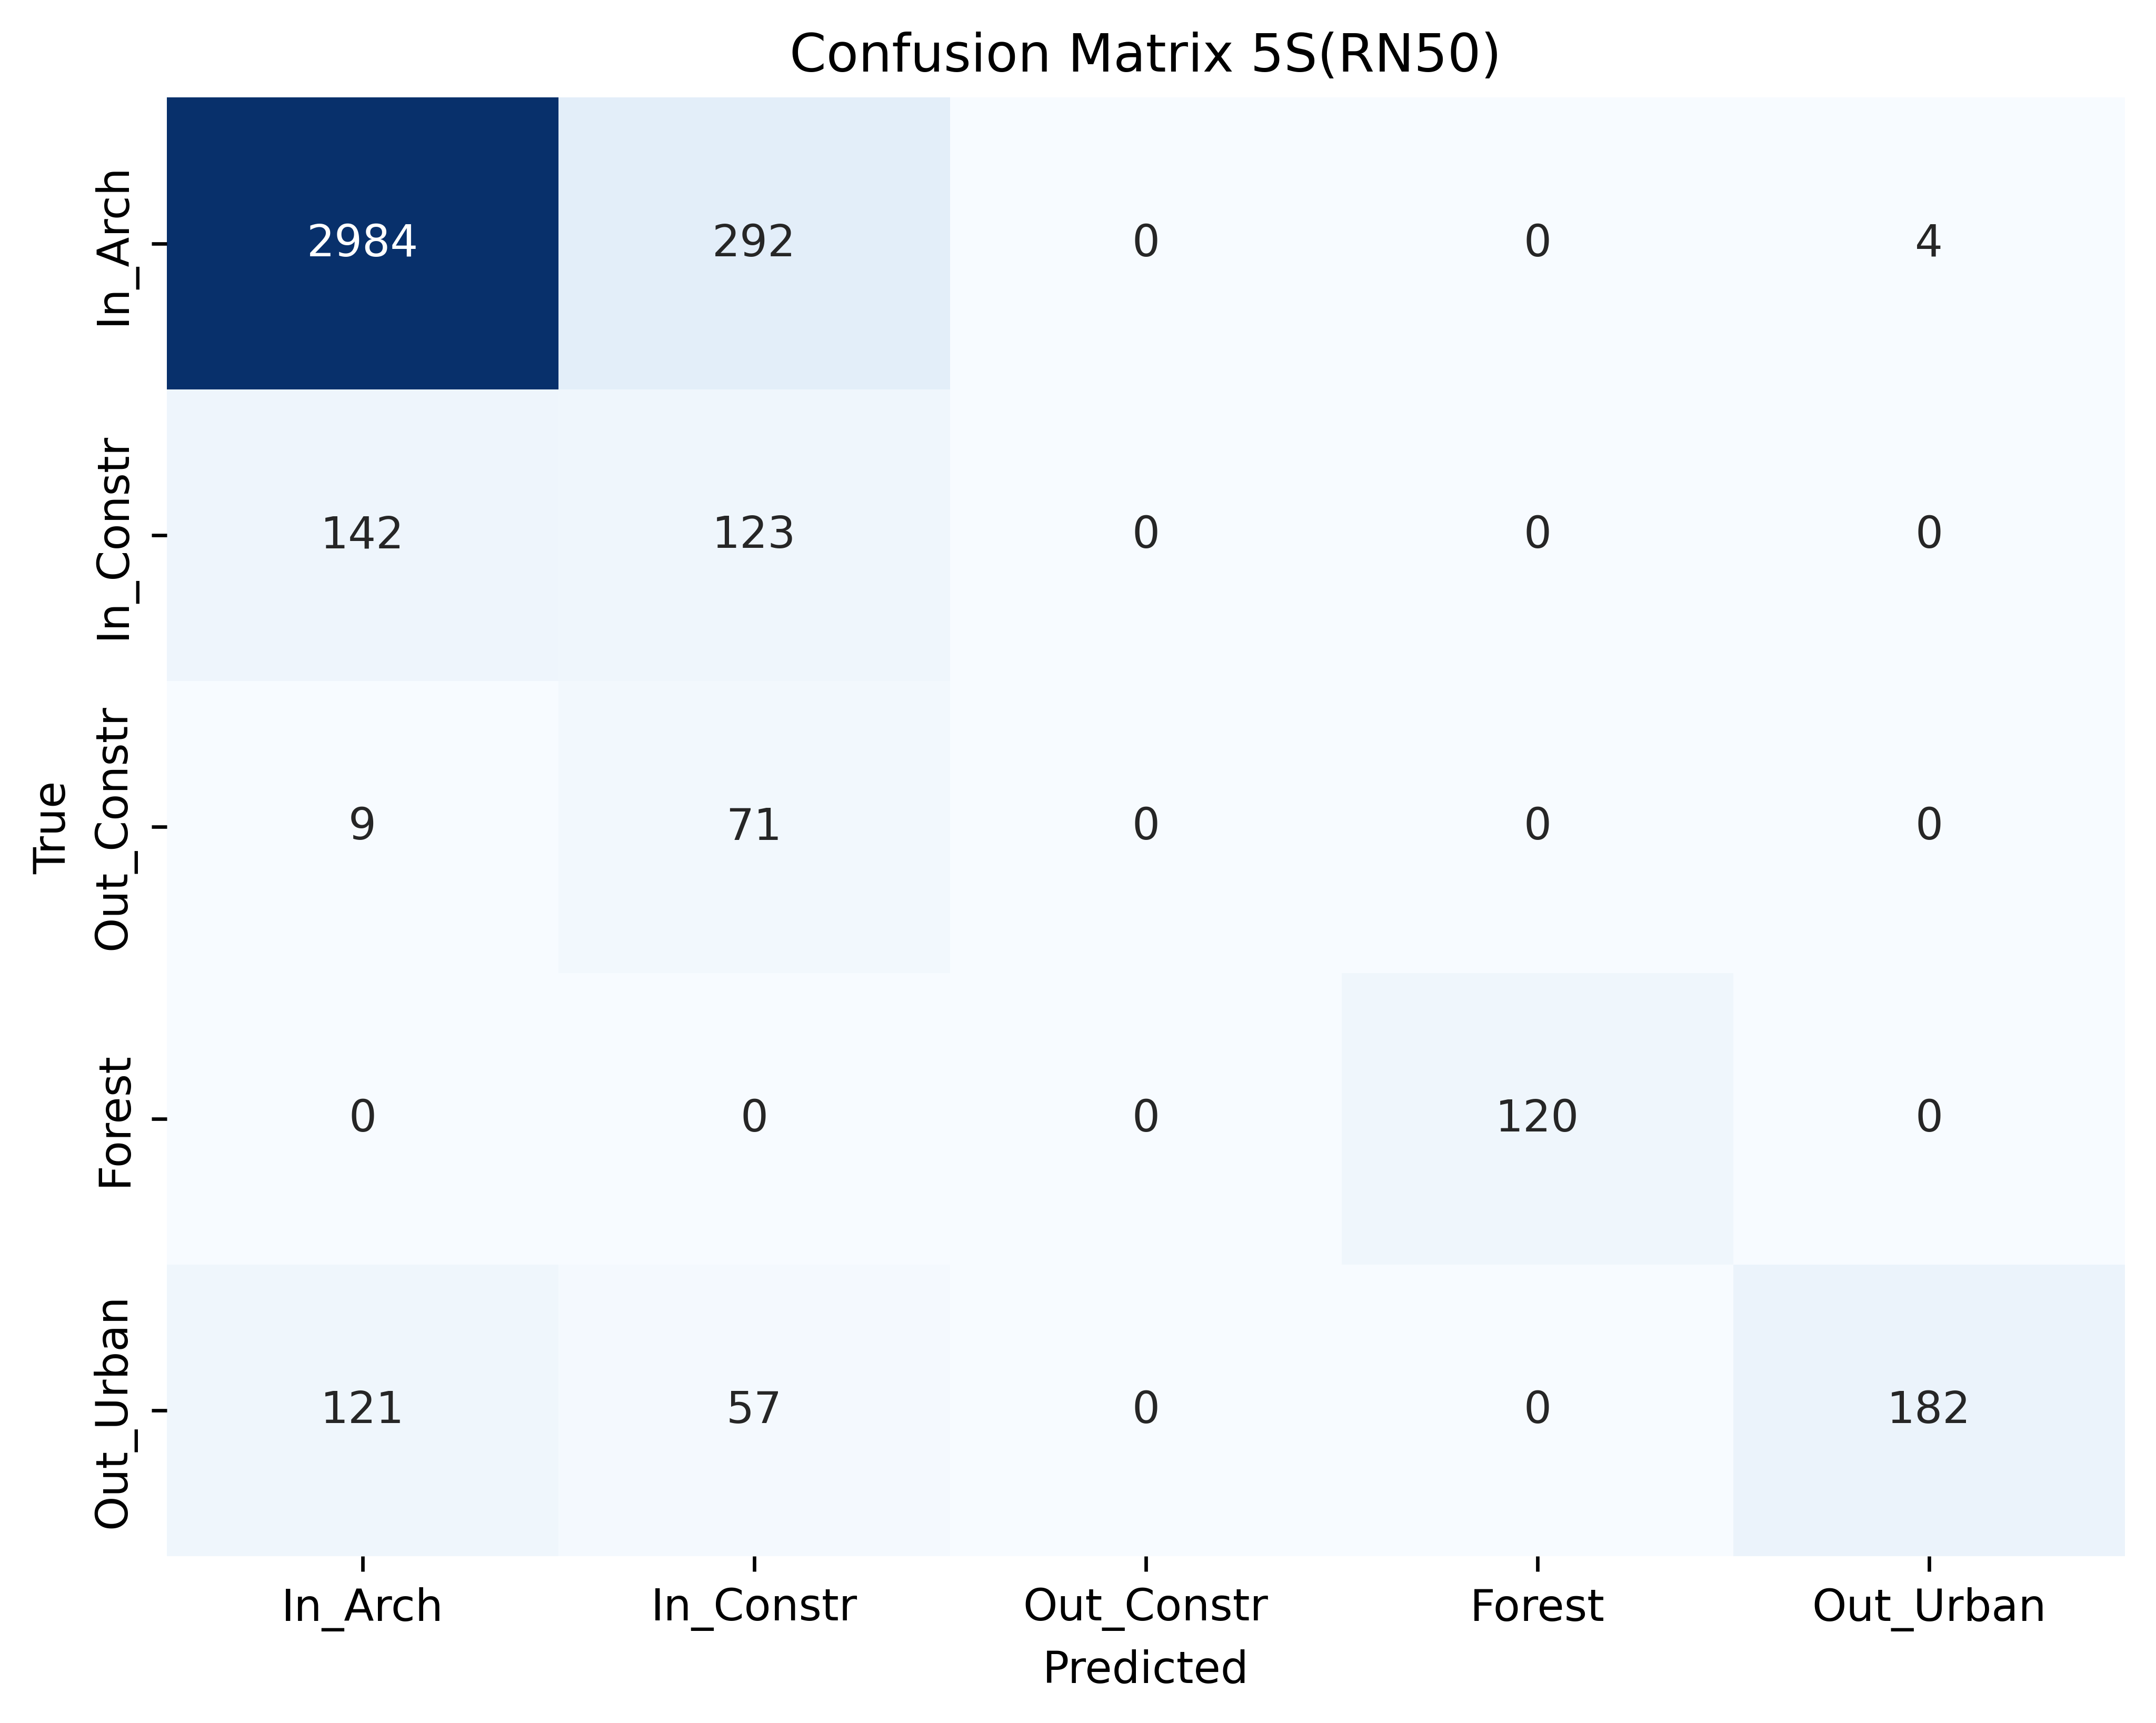
\includegraphics[width=0.45\textwidth]{Images/appendix/resultsRaspi/Confusion Matrix 5S(RN50).png}\label{resultpc:fig:rn505s}}
    \subfloat[][RN50x4]{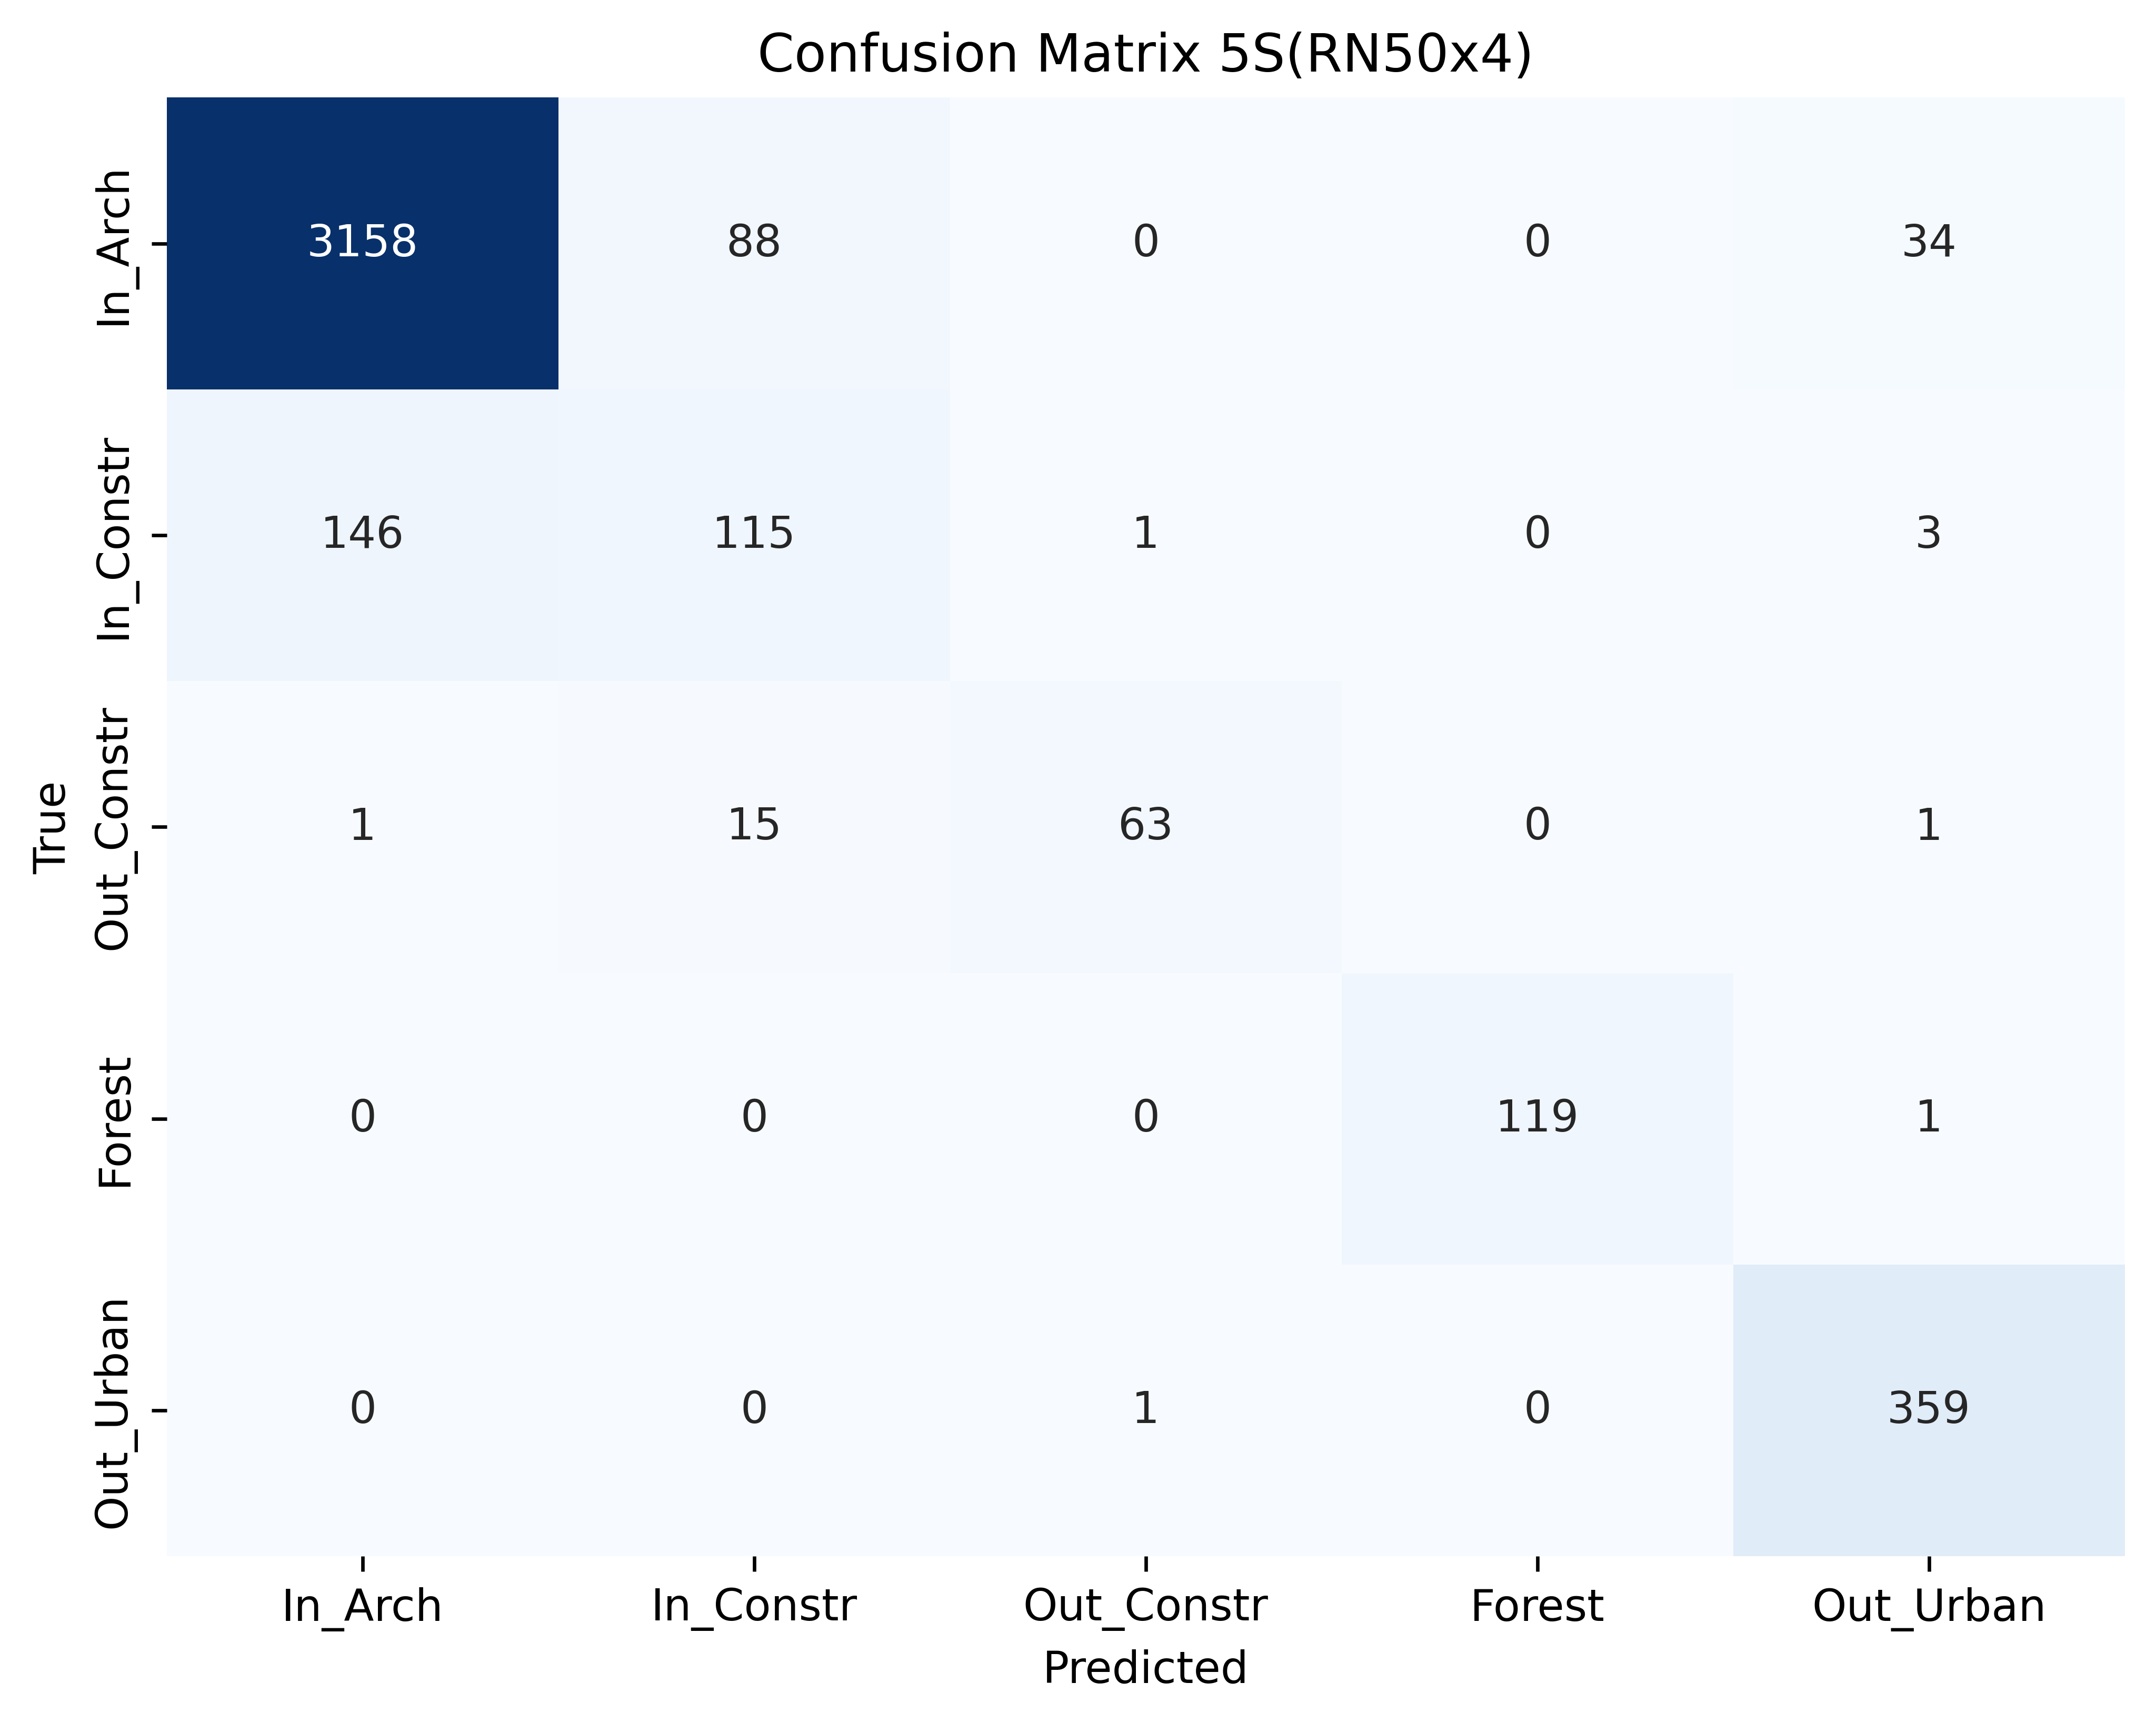
\includegraphics[width=0.45\textwidth]{Images/appendix/resultsRaspi/Confusion Matrix 5S(RN50x4).png}\label{resultpc:fig:rn50x45s}} \\
    \subfloat[][RN101]{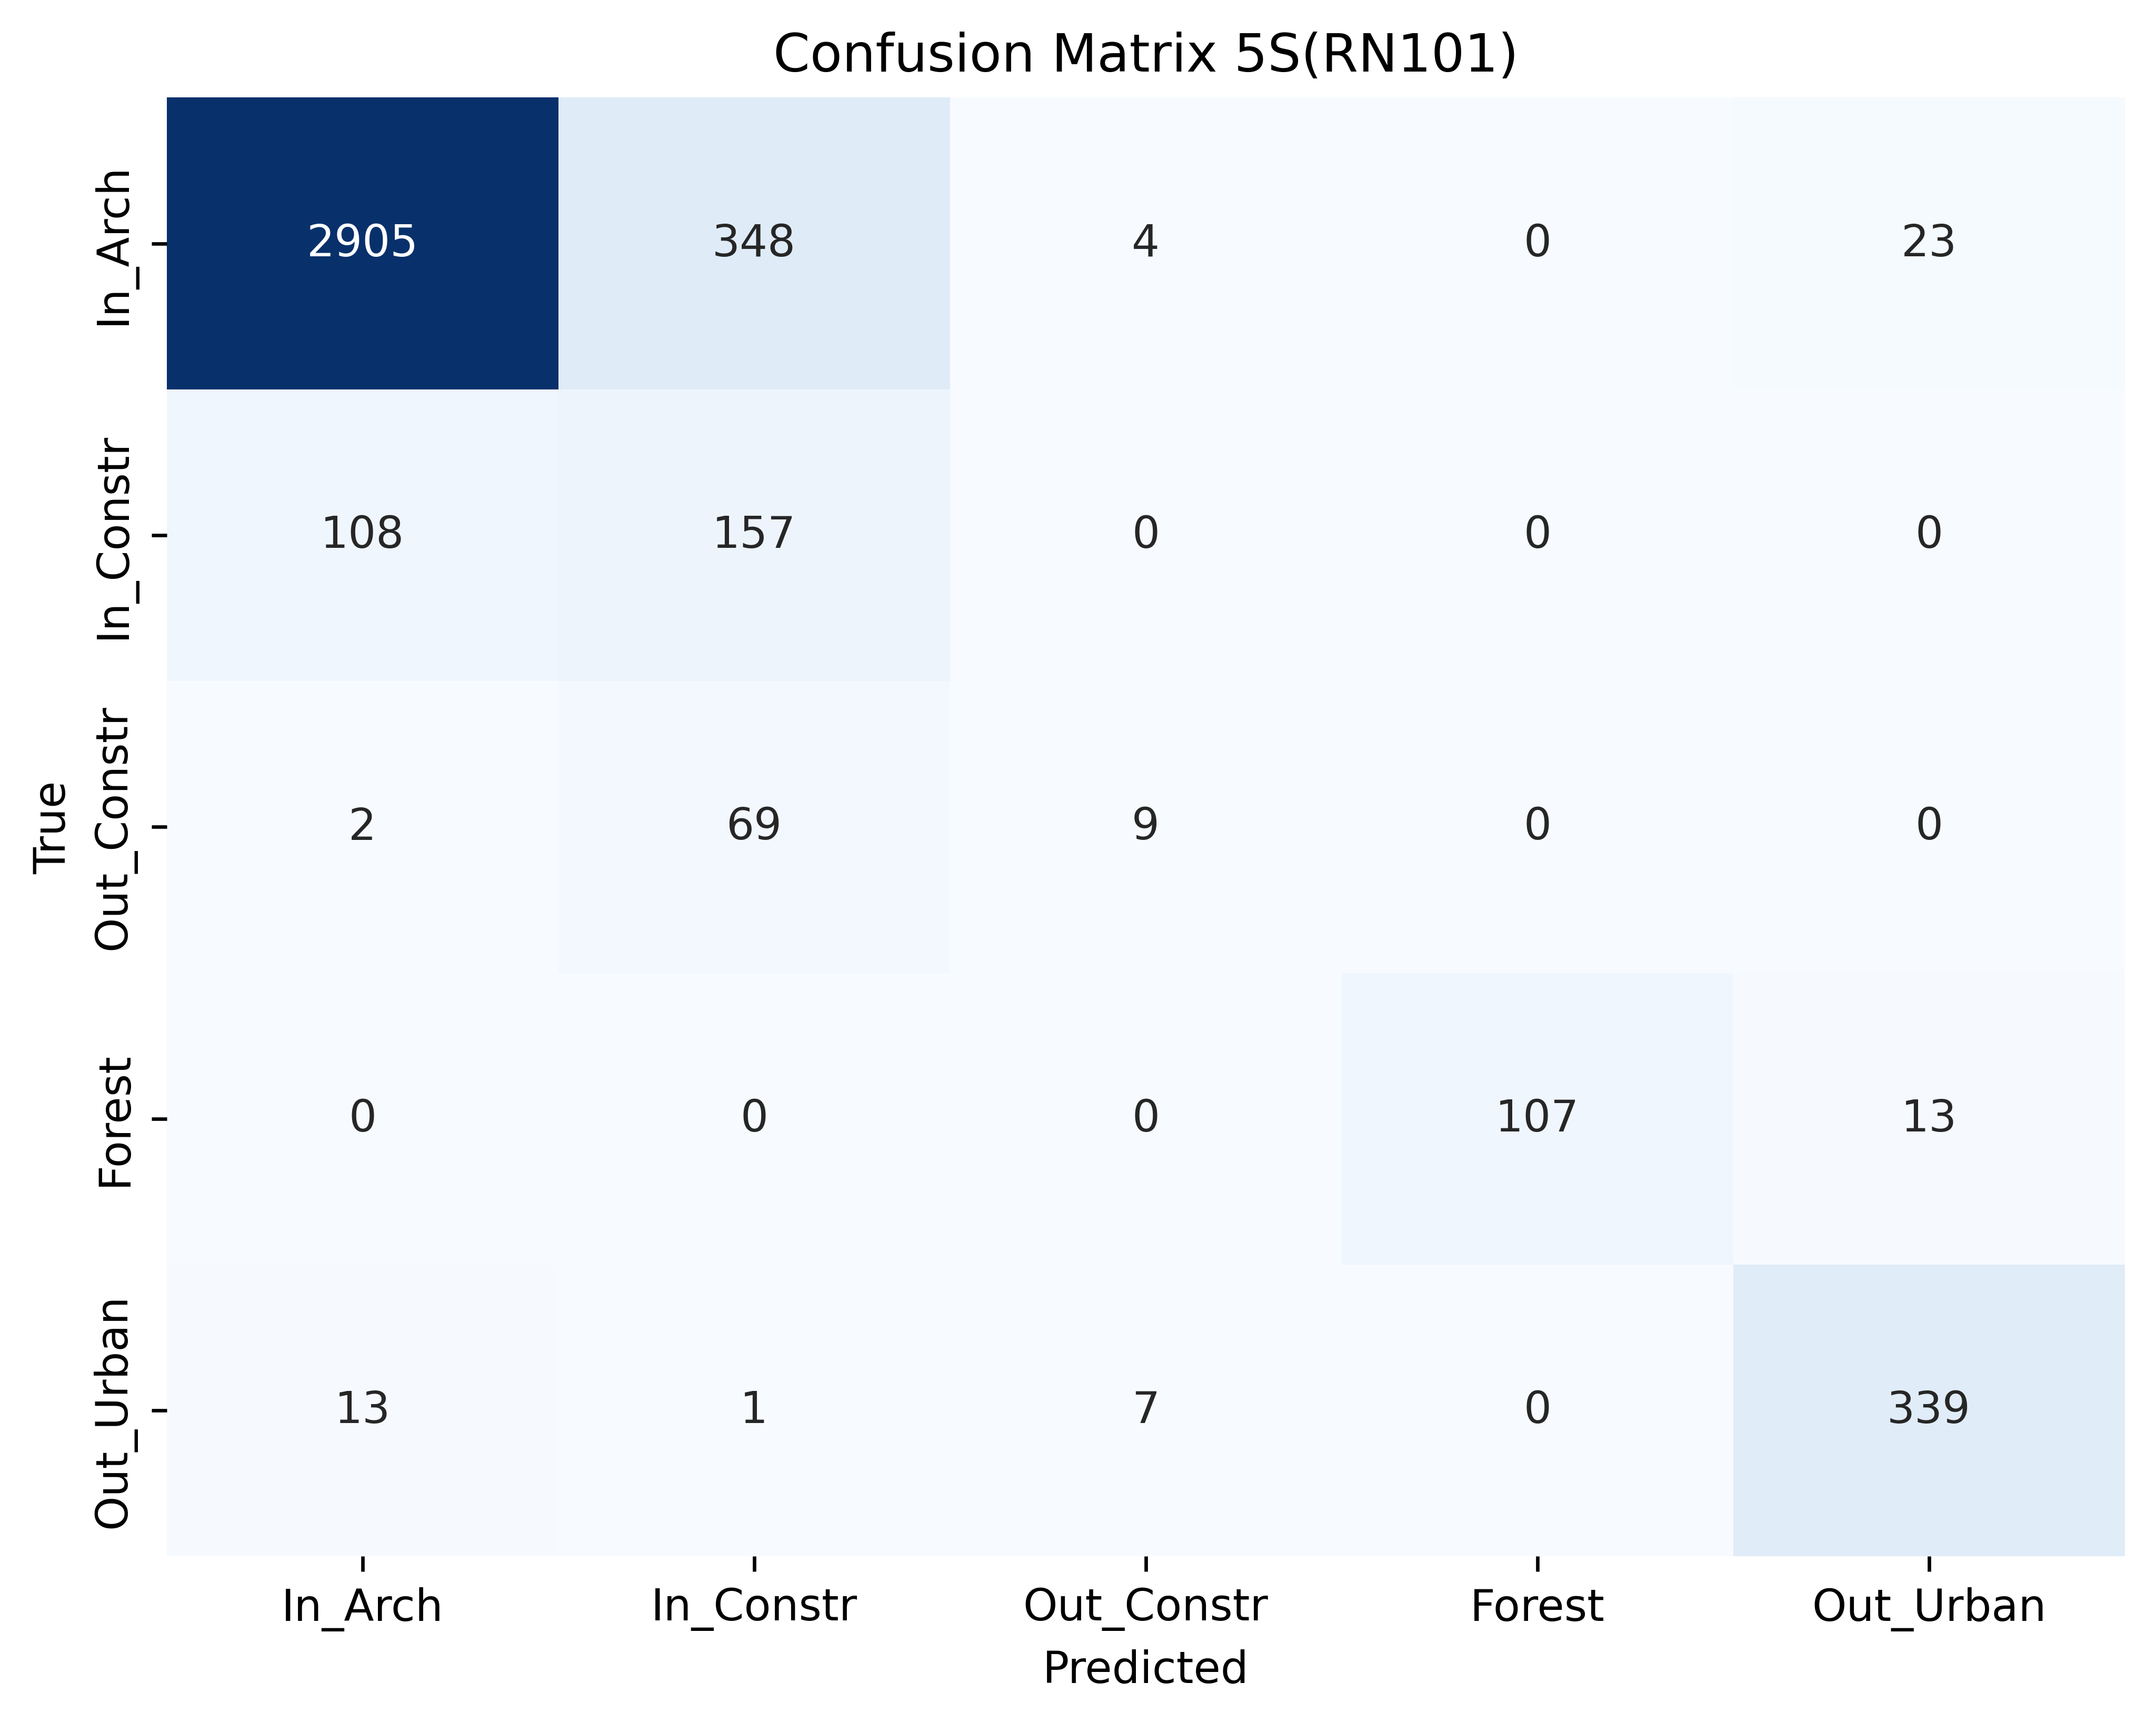
\includegraphics[width=0.45\textwidth]{Images/appendix/resultsRaspi/Confusion Matrix 5S(RN101).png}\label{resultpc:fig:rn50x645s}}
    \caption{Confusion Matrix on Raspberry Pi CPU for CLIP with ResNets as Visual Encoder (5 Sentences as Text Embeddings)}
    \label{resultpc:fig:clipevalraspi5s}
\end{figure}


    \chapter{ RE}
    \end{appendices}
    \newpage
    % Verzeichnisse
    \pagenumbering{alph}
    \listoffigures
    \listoftables
    \printbibliography
    \newpage
    
\end{document}

